% *============================================================================*
%                  UNIVERSITY OF MELBOURNE THESIS TEMPLATE
% *============================================================================*

% +----------------------------------------------------------------------------+
%  This is a Pandoc/LaTeX template for a University of Melbourne thesis designed
%  to be used as part of a bookdown project
%  (https://bookdown.org/yihui/bookdown/).
% +----------------------------------------------------------------------------+

% +----------------------------------------------------------------------------+
%  Changes:
%
%  2018-10-10 (Luke Zappia)
%    * Create first draft template
% +----------------------------------------------------------------------------+

% *============================================================================*
%  PREAMBLE
%
%  Set up the document, load packages, set parameters etc.
% *============================================================================*

% +-----Document class---------------------------------------------------------+
%  Set the class associated with the document, options in square brackets are
%  passed to the class
% +----------------------------------------------------------------------------+

\documentclass[11pt,a4paper,titlepage,twoside,openright]{style/unimelbthesis}

% +-----Packages---------------------------------------------------------------+
%  External packages used in the document
% +----------------------------------------------------------------------------+

\usepackage{graphicx}  % Extended graphics package.
\usepackage{amsmath}   % American Mathematics Society standards
\usepackage{amsxtra}   % Additional math symbols
\usepackage{amssymb}   % Additional math symbols
\usepackage{amsthm}    % Additional math symbols
\usepackage{latexsym}  % Additional math symbols
\usepackage{booktabs}  % Table formatting
\usepackage{longtable} % Table formatting
\usepackage{hyperref}  % Hyperlinks
\usepackage{setspace}  % Line spacing
\usepackage{chemarr}   % Improved reaction arrows for chemists
\usepackage{palatino}  % Use the palatino font family
\usepackage{mathpazo}  % Use the palotino font family

% +-----Parameters-------------------------------------------------------------+
%  Set parameters for the document. To convert from YAML to LaTeX we need to add
%  the dollar signs.
% +----------------------------------------------------------------------------+

\title{Managing Interacting Invasive Predators for Biodiversity Conservation}
\author{Matthew W. Rees}
\orcid{0000-0003-2549-3772}
\degree{Doctor of Philosophy}
\submissionmonth{September}
\submissionyear{2021}
\department{School of Ecosystem and Forest Sciences}
\university{The University of Melbourne}
\statement{Submitted in total fulfilment of the requirements of the degree of Doctor of Philosophy.}

% +-----Syntax highlighting----------------------------------------------------+
%  If code chunks are included in the document this allows Pandoc to insert the
%  code highlighting macros.
% +----------------------------------------------------------------------------+


% *============================================================================*
%  FRONT MATTER
%
%  Front section of the document, everything before the main text.
% *============================================================================*
\begin{document}
\begin{frontmatter}

% +-----Title------------------------------------------------------------------+

  \maketitle

% +-----Abstract---------------------------------------------------------------+
  \begin{abstract}
    Invasive predators are a major driver of global biodiversity loss. Accordingly, lethal invasive predator control is a common conservation strategy. However, despite usually being faced with multiple invasive predators, managers often implement targeted control of one species at a time due to feasibility constraints. There is concern that singular invasive predator control leads to a `mesopredator release' of subordinate predators, through relaxation via direct top-down pressure and indirect competition. An invasive mesopredators release could dampen or even worsen conservation outcomes. While intuitive, evidence for mesopredator release is weak due to a lack of robust experimental designs and replication, as well as reliance on activity indices.
    
    In this thesis, I investigated whether the lethal control of an apex invasive predator (red fox \emph{Vulpes vulpes}) has led to a mesopredator release of a widespread subordinate invasive predator (feral cat \emph{Felis catus}). I replicated field experiments and collated additional camera-trapping data across two regions with a simple predator guild comprising the introduced red fox and feral cat, allowing sharp focus on interactions between these species. Glenelg region with long-term fox control, Control-Impact with three replicates. Otway Ranges, BACIPS. I quantified impacts of fox control on two threatened native marsupials and assessed evidence for a mesopredator release of feral cats using multiple population metrics: site occurrence, spatiotemporal behaviour and population density.
    
    Fox occurrence strongly declined across the gradient of 1080 poison-bait density; the maximum of 20 baits deployed in a foxes home range reduced fox occurrence by 70\% consistently across both regions. However, this had basically no impact on southern brown bandicoot \emph{Isoodon obesulus} occurrence. Long-nosed potoroo \emph{Potorous tridactylus} occurrence increased with long-term fox-bait density in the Glenelg region, but decreased slightly in the Otway Ranges where fox control had recently commenced. Rather than being limited by foxes, habitat suitability for these threatened mammals was more strongly driven by an interaction between vegetation type and time since fire. However, not only do optimal fire regimes vary across species, but they can be entirely conflicting for the same species across different vegetation communities.
    
    At a landscape scale (mean size: 169 km\textsuperscript{2}), lethal fox control was associated with a range of responses from a negligible to 3.7-fold increase in feral cat density. Consistent with the mesopredator release hypothesis, the degree of increase corresponded with variation in the duration and intensity of fox suppression. At a fine spatial scale (200 m), feral cat density had a consistent negative association with fox occurrence across both regions. Individual cat detectability and movement also varied across the (artificially manipulated) fox occurrence gradient. Using a larger dataset without individual identification, I saw no evidence that foxes impacted the occurrence of cats, in fact, these predators were more likely to co-occur than not in the Glenelg region. Instead, feral cats seemed to avoid foxes by shifting diel activity patterns. Where foxes are nocturnal in the Glenelg region dry vegetation types of the Otway Ranges, cats became more active during the the day where fox activity was highest. In the wet vegetation types of the Otway Ranges where foxes were active consistently throughout the daily cycle; cats concentrated activity around midnight where fox activity was highest.
    
    My thesis provides replicated, experimental evidence that that apex predator suppression is associated with an increase in the density of a mesopredator. Mesopredator release can manifest as changes in both behaviour and density, distorting inference if these processes are not distinguished. Further, joint spatiotemporal models are required to adequately understand predator interactions. I provide an example of an easily implementable, hierarchical generalised additive model framework to investigate spatiotemporal changes in species detections and share information across different contexts. Our results help explain why fox control did not consistently improve southern brown bandicoot and long-nosed potoroo occurrence, suggesting integrated pest management may be necessary to improve conservation outcomes. Until thats feasible, maintaining habitat structure through careful use prescribed fire is a priority.
  \end{abstract}
% +-----Declaration------------------------------------------------------------+
  \begin{declaration}
    This is to certify that:
    \begin{enumerate}
    \def\labelenumi{\roman{enumi}.}
    \tightlist
    \item
      the thesis comprises only their original work towards the PhD except where indicated in the preface;
    \item
      due acknowledgement has been made in the text to all other material
      used; and
    \item
      the thesis is fewer than 100,000 words in length, exclusive of
      tables, maps, bibliographies and appendices.
    \end{enumerate}
  \end{declaration}
% +-----Preface----------------------------------------------------------------+
  \begin{preface}
    This preface provides a summary of the chapters in this thesis and describes my contribution to them as well as the contributions of my collaborators and supervisors. This is a thesis with publication and comprises four chapters that present my PhD research. Therefore there is some overlap in content and the pronoun `we' is used instead of `I' in recognition of the co-authors' contributions. The General Introduction provides a brief overview of the relevant literature and outlines the key themes underlying the research, while the Synthesis describes links between the papers and places the research in a broader context.
    
    I designed and led fieldwork to collect data for this PhD. I experimentally deployed 425 camera-traps in the Glenelg region during 2018 (a control-impact experiment two spatial replicates), and 524 camera-trap deployments in a Before-After-Control-Impact Paired series design in the western Otway Ranges from 2017 to 2019. I had field assistance from the following volunteers: Shauni Omond, Shayne Neal, Asitha Samarawickrama, Shelley Thompson, Erin Harris, Hannah Killian, Lani Watson, Mark Dorman, Jack Davis, Carl Roffey, Bruce Edley, Larissa Oliveira Gonçalves, Ben Lake, Chantelle Geissler, Aviya Naccarella, Emily Gronow, Harley England, David Pitts, Annie Hobby, Louise Falls, Thomas McKinnon, Jimmy Downie, Marney Hradsky, Stephanie Samson, Robin Sinclair, Asmaa Alhusainan, Kelly Forrester, Tammana Wadawani, Emily Gregg, Hannah Edwards, Adam Beck, Vishnu Memnon, Sandy Lu, Dr Pia Lentini, Prof.~Nick Golding, Emily McColl-Gausden, Nina Page, Maggie Campbell-Jones, Kyle Quinn and Jack Dickson. Surveys were conducted under University of Melbourne Animal Ethics Committee approval 1714119 and Victorian Government Department of Environment, Land Water and Planning Research Permit 10008273. I sorted camera-trap images and identified 133 individual feral cats from this dataset, with secondary independent identifications made by Mark Le Pla and Luke Woodford.
    
    Chapter 3 uses a subset of this dataset; the 2017 camera-trap deployments in the Otway Ranges. This dataset was used in its entirety for the other chapters, but was supplemented with additional data collected by government partner researchers (detailed below). Chapters 1 and 2 include an additional XX camera-trap deployments from the Glenelg Ark fox control monitoring program (2013-19) and XX from the Otway Ark fox control monitoring program (2016-18). Chapter 4 include an additional dataset from the Lower Glenelg National Park (serving as a third spatial replicate for the Control-Impact experimental design). Alan Robley designed this camera-trap layout, with Ethan Le Duc, Michael Murrell, Dylan Thomas, Rhys Weber, Chris Johansson, Lachlan Levings and Liz Beever carried out the surveys, with Luke Woodford identifying cats (all from the Victorian Government Department of Environment, Land, Water and Planning).
    
    \(~\)
    
    \hypertarget{publications-included-as-part-of-this-thesis}{%
    \section*{Publications included as part of this thesis}\label{publications-included-as-part-of-this-thesis}}
    \addcontentsline{toc}{section}{Publications included as part of this thesis}
    
    \textbf{Chapter 1}
    
    Contributions:
    
    Code:
    
    \(~\)
    
    \textbf{Chapter 2}
    
    Contributions:
    
    Code:
    
    \(~\)
    
    \textbf{Chapter 3}
    
    MW Rees, JH Pascoe, BA Wintle, M Le Pla, EK Birnbaum, BA Hradsky (2019). Unexpectedly high densities of feral cats in a rugged temperate forest. \emph{Biological Conservation}, \textbf{239}, 108287.
    
    Contributions:
    
    Code: \url{https://github.com/matt-w-rees/feral-cat-otways-2017-SMR}
    
    \(~\)
    
    \textbf{Chapter 4}
    
    \textbf{MW Rees}, JH Pascoe, M Le Pla, A Robley, EK Birnbaum, BA Wintle, \& BA Hradsky (\emph{In review}). Quantifying mesopredator release: lethal control of an invasive apex predator alters feral cat density and detectability.
    
    Contributions: M.W.R, B.A.H, J.H.P, B.A.W and A.R conceived the ideas and designed the methodology; M.W.R, J.H.P, M.LP, E.K.B and B.A.H collected the data; M.W.R analysed the data with input from B.A.H and B.A.W, and led the writing of the manuscript. All authors contributed critically to the drafts and gave final approval for publication.
    
    Code: \url{https://github.com/matt-w-rees/invasive-mesopredator-release}
    
    \newpage
    
    \hypertarget{other-publications-that-i-have-contributed-to-during-my-candidature-but-are-not-presented-in-this-thesis}{%
    \section*{Other publications that I have contributed to during my candidature but are not presented in this thesis}\label{other-publications-that-i-have-contributed-to-during-my-candidature-but-are-not-presented-in-this-thesis}}
    \addcontentsline{toc}{section}{Other publications that I have contributed to during my candidature but are not presented in this thesis}
    
    M Le Pla, EK Birnbaum, \textbf{MW Rees}, BA Hradsky, AR Weeks, A Van Rooyen, JH Pascoe (\emph{In review}).
    Genetic Sampling and an Activity Index Indicate Contrasting Outcomes of Lethal Control for an Invasive Predator
    
    A Stobo-Wilson, BP Murphy, SM Legge, DG Chapple, HM Crawford, SJ Dawson, CR Dickman, TS Doherty, PA Fleming, M Gentle, TM Newsome, R Palmer, \textbf{MW Rees}, EG Ritchie, J Speed, J Stuart, E Thompson, J Turpin, JCZ Woinarski (\emph{In review}). Compounding and complementary carnivores: Australian bird species eaten by the introduced European red fox Vulpes vulpes and domestic cat \emph{Felis catus}.
    
    A Stobo-Wilson, BP Murphy, SM Legge, DG Chapple, HM Crawford, SJ Dawson, CR Dickman, TS Doherty, PA Fleming, M Gentle, TM Newsome, R Palmer, \textbf{MW Rees}, EG Ritchie, J Speed, J Stuart, E Thompson, J Turpin, JCZ Woinarski (2021). Reptiles as food: predation of Australian reptiles by introduced red foxes compounds and complements predation by cats. \emph{Wildlife Research} \textbf{48}, 470-480. \url{https://doi.org/10.1071/WR20194}
    
    A Stobo-Wilson, BP Murphy, HM Crawford, SJ Dawson, CR Dickman, TS Doherty, PA Fleming, M Gentle, SM Legge, TM Newsome, R Palmer, \textbf{MW Rees}, EG Ritchie, J Speed, J Stuart, E Thompson, J Turpin, JCZ Woinarski (2021). Sharing meals: Predation on Australian mammals by the introduced European red fox compounds and complements predation by feral cats. \emph{Biological Conservation} \textbf{261} : 109284. \url{https://doi.org/10.1016/j.biocon.2021.109284}
    
    H Davies, Tiwi Land Rangers, \textbf{MW Rees}, D Stokeld, AC Miller, GR Gillespie, BP Murphy (2021). Variation in feral cat density between two large adjacent islands in Australia's monsoon tropics. \emph{Pacific Conservation Biology}. \url{https://doi.org/10.1071/PC20088}
    
    \textbf{MW Rees}, J Carwardine, A Reeson, and J Firn (2020). Rapidly assessing cobenefits to advance threat-management alliances. \emph{Conservation Biology}, \textbf{34}: 843-853. \url{https://doi.org/10.1111/cobi.13490}
  \end{preface}
% +-----Acknowledgements-------------------------------------------------------+
  \begin{acknowledgements}
    I acknowledge and pay respect to the Gadubanud and Gunditjmara people on whose traditional lands this study took place. It was a privilege to learn about and work on across the countries.\\
    I also completed my PhD while living on Wurundjeri country and Bandjalang country.
    
    Supervisors.
    
    Committee.
    
    Discussions many QAEco people highly influenced this PhD. Zoï. Plus Billy.
    
    This thesis would be very different--much worse--without the assistance of nearly 50 fieldwork volunteers.
    Vin and Kelly provided me a home away from home during fieldwork and some much needed employment.
    
    Heywood DELWP office. Wes and the revolving troop of GA project officers: Pittsy, Thomas McKinnon, Lou, Ethan.
    Glenelg Ark, Arthur Rylah Institute for borrowing camera-traps.
    Claire Miller from PV Otway Ark.
    
    Family and friends. Particularly parents. Cara.
    
    Funding:
    Our study was generously supported by the Conservation Ecology Centre, the Victorian Government Department of Environment, Land Water and Planning, Arthur Rylah Institute for Environmental Research, Parks Victoria, the Australian Government's National Environmental Science Program through the Threatened Species Recovery Hub, and ARC Linkage Project LP170101134. M.W.R also receives support from an Australian Government Research Training Program Scholarship.
  \end{acknowledgements}
% +-----Table of contents------------------------------------------------------+

  \hypersetup{linkcolor=black}
  \setcounter{tocdepth}{2}
  \tableofcontents

% +-----List of tables---------------------------------------------------------+

  \listoftables

% +-----List of figures--------------------------------------------------------+

  \listoffigures

% +-----List of copyright------------------------------------------------------+
\begin{copyrightlist}
  List of all third party copyright material included in the thesis and whether
  permissions have been obtained to include this content in the open access
  version of the thesis.
\end{copyrightlist}
\end{frontmatter}
% *============================================================================*
%  MAIN MATTER
%
%  Main part of the document. Includes all chapters and appendices.
% *============================================================================*

\begin{mainmatter}

\hypertarget{general-introduction}{%
\chapter*{General Introduction}\label{general-introduction}}
\addcontentsline{toc}{chapter}{General Introduction}

Welcome to my University of Melbourne \emph{R Markdown} thesis template.

\hypertarget{occ}{%
\chapter{Fire and poison-baiting manipulate invasive predator and threatened prey occurrence within temperate landscapes}\label{occ}}

\hypertarget{abstract}{%
\section*{Abstract}\label{abstract}}
\addcontentsline{toc}{section}{Abstract}

\newpage

\hypertarget{introduction}{%
\section{Introduction}\label{introduction}}

Conservation managers intervene with ecosystems to stem rapid biodiversity loss, but benefits are rarely quantified. Understanding management outcomes is essential to ensure cost-effectiveness and detect potential unintended consequences. However, reliable inference is difficult to achieve because management effects need to be separated from `natural' drivers and population fluctuations, as well the impact of co-occurring threats and management. Further, we often have a poor understanding of what drives the patchy occurrence of species within their distributions--the spatial scale at which management usually operates at, and a common metric used to evaluate conservation strategy success.

Australian native terrestrial mammals have experienced some of the worst declines in recent history. While habitat destruction is a key threatening process, mammalian extinctions have largely taken place within large tracts of native vegetation. Mammals weighing between 35 and 5500 g (`critical weight range') have been hit hardest as they are the preferred meal size for both the red fox \emph{Vulpes vulpes} (hereafter `fox') and feral cat \emph{Felis catus} (hereafter `cat'), introduced following European invasion more than 230 years ago. Concurrently, widespread dispossession of Indigenous lands has interrupted at least 65,000 years of traditional land management, particularly using fire, causing dramatic ecosystem change. More recently, native mammal population have succumbed to extended periods of reduced rainfall and drought. Invasive predators, altered fire regimes and climate change have hit Australia hard, but are also pervasive threats to global biodiversity. To prioritise threat-management within protected areas, conservationists require finescale information on native prey threat susceptibility and responses to threat-management across heterogeneous environments.

Invasive predators are a management focus as they are significant drivers of both biodiversity and economic loss. More land in Australia has been managed for foxes than any other invasive vertebrates, primarily through continuous 1080 poison-baiting (Saunders, Gentle, \& Dickman, 2010). However, native prey benefits are rarely demonstrated. This is partly because fox control programs go unmonitored, or monitoring provides limited inference on native prey responses (reddiex), and partly because dramatic declines and local extinctions have been reported after long-term fox control (e.g.~wayne; lindenmeyer; grampians; rock wallabies). This may be due to insufficient control effort to suppress fox to a level which benefits prey, or because fox suppression has `released' feral cats (i.e., mesopredator release). However, we have little empirical evidence for either alternative. Few studies have quantified fox suppression across a gradient of control effort. Feral cats do appear to increase abundance following fox control, although there is considerable uncertainty around this (Hunter). Evaluating fox control is difficult due to co-occuring threats and management actions.

Minimising the threat of large wildfires is an increasingly important role of land managers. Large wildfires are generally mitigated at the landscape scale through small-scale controlled burns to reduce fuel-loads (dried vegetative substrate). Prescribed burning operations require juggling asset protection against the often competing needs of native species. While some animals may succumb to direct mortality from fire events, most impacts are indirect through longer-term changes food and habitat resources. Animals response to fire are often measured using time since the last fire event, however, post-fire regeneration varies considerably across different vegetation communities. While sample sizes often prohibit estimating fire responses across different contexts, it is imperative to inform optimal fire regimes across heterogeneous landscapes.

Rainfall dynamics impact habitat suitability over time. Animals may occur widely across across their distributions, but dramatically contract to small areas which offer refuge during dry periods. These rainfall-induced population dynamics are well documented in regions with irregular rainfall (Pavey et al.~2017), but there is increasing evidence that similar patterns occur in temperate ecosystems (e.g.~Hale 2016). Understanding how rainfall triggers changes in species occurrence dynamics--and how this varies across space--is a large step towards separating environmental drivers from intervention outcomes, as well as to effectively prioritise management where and when it most needed.

Fire and rainfall dynamics are near-ubiquitous drivers of mammal populations, but are seldom been accounted for assessing fox control outcomes. For example Boodoree, western shied\ldots{} Experimental designs are called for to improve inference, but are not immune to these confounding effects. This is highlighted by the Glenelg Ark program; using a Before-After-Control-Impact paired series experimental design with three spatial replicates makes it the most robustly monitored fox control experiment in Australia. However, fox control commenced during the millenium drought and landscapes subject to fox control have been the most frequently burnt--the reality of conducting broad-scale management experiments in-situ. These confounding factors, or perhaps a mesopredator release of feral cats, may explain why two threatened native prey species, the southern brown bandicoot \emph{Isoodon obesulus} (hereafter `SBB') and long-nosed potoroo \emph{Potorous tridactylus} (hereafter `LNP'), have had an inconsistent, underwhelming response to fox control in the Glenelg region, Australia.

Here, we quantified changes in invasive predator and threatened native prey occurrence across 1080 poison-bait density gradients for two broadscale fox control programs, while accounting for the effects of rainfall and fire. From 3667 camera-trap deployments over seven years, we were able to survey mammals across a range of environmental conditions and management contexts across two broad regions implementing fox control in south-west Victoria, Australia. We used generalised additive models to fit nonlinear relationships between fox, cat, SBB and LNP occurrence and several spatial and temporal covariates, including (1) fox-bait density, (2) time since fire across vegetation communities, (3) rainfall with short and long-term interactions. We hypothesised that: (1) fox-bait density would be associated with declines in fox occurrence, increases in SBB, LNP and cat occurrence (in accordance with the mesopredator release hypothesis), (2) species occurrence would vary with time since fire, but in slightly different ways across vegetation communities, (3) species occurrence would increase during periods of high rainfall, but more greatly in areas with low long-term rainfall. We also accounted for habitat fragmentation, hypothesising that (4) predator occurrence would highest closest to cleared edges, and that threatened prey occurrence would be lowest here.

\newpage

\hypertarget{methods}{%
\section{Methods}\label{methods}}

\hypertarget{study-area}{%
\subsection{Study area}\label{study-area}}

We collated camera-trap data across the Glenelg region and Otway Ranges in south-west Victoria, Australia (Fig. \ref{fig:occ-map}). The terrestrial mammalian predator guild is depauperate throughout both regions; native dingoes \emph{Canis familiaris} are long absent throughout, tiger quolls \emph{Dasyurus maculatus} are long-absent in the Glenelg region and likely functionally extinct in the Otway Ranges (last confirmed sighting in 2014 despite extensive camera-trapping). Introduced foxes and cats are therefore the only medium-large functional mammalian terrestrial predators across both regions. The purpose of each collated study was to experimentally survey changes in the mammalian community due to fox control. In broad sections of each region, government land managers conduct ongoing targeted fox control for biodiversity conservation. Poison baits containing 3 mg of sodium mono-fluroacetate (`1080') are buried at a depth of 10 cm at 1-km intervals along accessible forest tracks and roads. This allowed us to investigate fox-cat interactions across a gradient of apex predator (fox) activity and other landscape contexts. Prescribed fire is another key management action undertaken throughout both regions (except in very wet sections of Otway Ranges), primarily for asset protection.

In the Glenelg region, Gunditjmara country, natural vegetation--mostly lowland forests and heathy woodlands--is fragmented (Fig. \ref{fig:occ-map}). Foxes have been subject to lethal control in three distinct forest blocks (separated by pastoral farming and residential property) since October 2005, with 1080 poison-baits replaced fortnightly (Robley \emph{et al.} 2014a). Three similar, but unbaited, forest blocks to the north have been surveyed simultaneously as an experimental control (Robley \emph{et al.} 2014a).

The Otway Ranges, Gadubanud country, is a largely continuous patch of natural vegetation with a strong east-west rainfall gradient. A matrix of cool temperate rainforest and wet forest in the high-altitude south-west descends into a large heathland directly north, and into dry forests and then heathlands to the north-east. Foxes are controlled through 1080 poison-baits with monthly replacement across most of the Otway Ranges, but a large section to the north-west remains unbaited. The majority of this baiting began in 2016 - 2017, although fox-baiting commenced in some small sections in 2008.

\hypertarget{camera-trap-surveys}{%
\subsection{Camera-trap surveys}\label{camera-trap-surveys}}

We compiled camera-trap data from three distinct studies across the two regions; totalling 3667 deployments of camera-traps at 1232 camera-trap sites. Camera-traps were active for an average of 47 days, totalling 172,052 trapnights. Camera-trap spacing was variable; the average minimum distance between simultaneously deployed camera-traps was 445, 853 and 1266 metres for each study. Camera-traps were deployed in the Glenelg region between 2013 -- 2019, and in the Otway Ranges between 2016 -- 2019.

All camera-trap deployments consisted of a Reconyx (Holmen, Wisconsin) brand camera-trap (both white and infrared flash), attached to a tree or a metal picket, facing a lure. Camera-traps were set-up in two ways depending on the key aim of the project, either targeted toward predators or prey species. One study across both regions positioned camera-traps lower on a tree (around 15 - 30 cm above the ground -- angled only slightly downwards) facing a tuna oil lure approximately 2 - 2.5 m away (detailed in Rees \emph{et al.} 2019). The remaining camera-traps were positioned higher on a tree or a metal picket (at least 40 cm above ground) and angled downwards more strongly - facing a lure approximately 1 - 1.5 m away. These lures consisted of peanut butter, golden syrup and rolled oats mixed into a small ball, placed within a tea strainer or PVC pipe container and secured either to the ground, or 20 - 60 cm above ground on a wooden stake. All set-ups were effective in detecting both predator species.

\hypertarget{cumulative-detection-probabilities}{%
\subsection{Cumulative detection probabilities}\label{cumulative-detection-probabilities}}

We did not incorporate imperfect detection in the GAMs. To determine the bias this may have had, we calculated the cumulative probability of detection by fitting a single season occupancy-detection model (MacKenzie et al.~2002). We fit these models using the `unmarked' R-package with 24-hour sampling occasions. We then calculated the calculated the probability that each species would have been detected for a given survey duration (Garrard \emph{et al.} 2008) of up to 93 days (the maximum survey duration).

\hypertarget{generalised-additive-models-of-species-occurrence}{%
\subsection{Generalised additive models of species occurrence}\label{generalised-additive-models-of-species-occurrence}}

We constructed a table with a row for each camera-trap deployment, a presence-absence column for each of the four study species, as well as additional columns for site information and explanatory variable values. We modelled occurrence probability for each species (response variable) using binomial generalised additive mixed-effects models implemented in the `mgcv' R-package (Wood 2017). We specified a model offset to account for differences in camera-trap survey durations and a random intercept for each unique site to account for repeat sampling. We used the same model structure for each species, because we expected all species to be effected by these explanatory variables and we aimed to contrast responses. We used the double penalty model selection approach, which penalises the null space in addition to the range space (i.e.~shrinking wiggly terms to linear terms) of the spline basis, meaning covariate effects can be entirely removed from the model (Marra \& Wood 2011).

We expected the density of 1080 poison-baits (targeted to foxes) to decrease the fox occurrence probability, and therefore increase the occurrence probability of three subordinate species. We summed the number of fox-baits within a 2.3 km radius around each camera-trap deployment - the average maximum distance foxes in these region travel from their home range centre (Hradsky \emph{et al.} 2017). We modelled this explanatory variable using a thin plate regression spline, with a factor smooth basis to model the impact separately for each region: poison-baits are replaced at different frequencies (fortnightly v.s monthly) across the regions, which has been occurring over different time scales (\textasciitilde7-13, 0-3 years) in the Glenelg region and Otway Ranges (respectively).

We surveyed species across a range of vegetation community types, which provide different levels of food and shelter. However, these resources are mediated by fire, but regeneration following fire occurs occurs at different speeds across vegetation types (McColl-Gausden \& Penman 2019). We expect species occurrences to differ across vegetation types and with time since fire, but to have slightly different responses to time since fire in each different vegetation type; we therefore modelled an interaction between time since fire (in years; hereafter `TSF'). We used coarse fire scar mapping provided by government managers to calculate the years since the last fire for each camera-trap deployment. We attached Ecological Vegetation Class (hereafter ``EVC''; standard units for vegetation classification in Victoria; DELWP 2020) groups for each unique camera-trap site, 8 EVC groups in total. We surveyed 20 unique sites in rainforests, which are interspersed (primarily in low lying gullies) throughout wet and damp forests in the south-eastern Otway Ranges. Given the similarity and finescale interspersion of these EVC groups, and that both rarely or never experience fire, we merged them together (hereafter referred to as `wet forests'). We specified this a hierarchical model structure, which estimated an average TSF response (`global smoother'), along with EVC group-level smoothers with shared wiggliness (i.e.~model GS in Pedersen \emph{et al.} 2019) This shares information on TSF responses across groups and penalises functions which deviate strongly from the average response--increasing confidence that they are true deviations opposed to the result of sampling noise.

Long-term climate is a strong driver of species distribution in the Otway Ranges (Swan \emph{et al.} 2021), as are short-term rainfall fluctuations in another region of south-western Victoria (Hale \emph{et al.} 2016). We expect short-term rainfall fluctuations to have different impacts across the wide spatial gradient of average rainfall in our study sites. We therefore modelled a tensor product interaction term for spatial annual average rainfall and short-term temporal dynamics in actual rainfall. We extracted annual rainfall values (mm) from the NARCLiM dataset (1-km resolution)\href{\%22https://app.bccvl.org.au/datasets?iframe\#c12=modified\&reversed=on\&b_start=0\&c2=4816d016b9af4fb18f6cc8b2f1f979dc\%22}{BCCVL database}. To calculate percentage different in short-term rainfall, we downloaded all available rainfall data from proximal weather stations (n = XX) from \href{\%22https://www.longpaddock.qld.gov.au/silo/point-data/\%22}{Queensland Government and the Australian Bureau of Meteorology}. For each species detection, we took the amount of rainfall in the previous 18 months at the nearest weather station, as well as the median rainfall over that same 18 month period since rainfall began being recorded at that weather station, and calculated the percentage difference between those two values. We chose 18 months for a comparison to Hale \emph{et al.} (2016)).

Invasive predators are well-documented to prefer edges between forest and cleared land (refs). Mammalian prey species are also likely impacted by edges indirectly due to increased invasive predators occurrence probability, and directly due to lower level of proximal suitable habitat (refs). We inverted the Victoria native vegetation extent shapefile from \href{\%22https://discover.data.vic.gov.au/dataset/native-vegetation-modelled-2005-ecological-vegetation-classes-with-bioregional-conservation-sta\%22}{DELWP}, and removed non-native vegetation areas which were smaller than 30 ha (which Hradsky ref?). For each camera-trap site, we calculated the minimum distance to non-native vegetation area. We used a thin plate regression spline for this smooth.

All analyses were conducted in R version 3.6.3 (R Core Team 2020).

\newpage

\(~\)

\(~\)

\(~\)
\begin{figure}

{\centering \includegraphics[width=1\linewidth]{figure/c1/fig1_map} 

}

\caption{Locations of study sites in south-west Victoria, Australia. The grids of camera-traps are denoted by white dots. The Glenelg region is to the west and Otway region to the east. Native vegetation is indicated by dark green, with hill shading. Map tiles by Stamen Design, under CC BY 3.0, map data by OpenStreetMap, under CC BY SA.}\label{fig:occ-map}
\end{figure}
\newpage

\hypertarget{results}{%
\section{Results}\label{results}}

Fox occurrence declined with increasing poison-bait density, but this relatively weak effects on the other mammal species (Fig. \ref{fig:occ-1080}). The maximum poison-bait density, 9 baits per km\textsuperscript{2}, reduced fox occurrence probability, consistently across both regions, by \textasciitilde75\% (Fig. \ref{fig:occ-1080}). This was a linear decline in the Otway region, but a nonlinear shape in Glenelg with diminishing bait returns from 3 - 6 baits km\textsuperscript{-2}. We saw no effect on fox control on cat occurrence across both regions. Fox-baiting slightly increased SBB and LNP occurrence in the Glenelg region, but slightly decreased their occurrence in the Otway region. The impact on SBB's was negligible; LNP's in the Glenelg region benefited the most from fox control (Fig. \ref{fig:occ-1080}c-d).

Threatened species occurrence was most strongly driven by vegetation type and fire (Fig. \ref{fig:occ-tsf}). Despite being detected across all all vegetation communities, the majority of SBB and LNP detections took place in heathy communities; lowland forests were also important for SBB's, while herb-rich woodlands were also important for LNP's (Table \ref{tab:occ-naive}). However, within these vegetation communities, occurrence probability varied substantially with TSF for both threatened species. SBB's had the most complex interactions with TSF, with occurrence peaking 20 and 75 years post-fire, although the strength of the 75 year peak varied considerably across vegetation communities. Potoroo occurrence increased linearly with TSF in heathy landscapes, but decreased linearly with TSF in herb-rich woodlands. TSF on this long-term scale had a weak impact on invasive predators, and foxes were also relatively unaffected by EVC group (Fig. \ref{fig:occ-tsf}). Foxes, cats, and LNP's had a near-flat global function for average TSF. Foxes also had flat functions for TSF in each EVC group, whereas cats and LNP occurrence had variable relationships with TSF across the EVC groups.

Foxes were most strongly impacted by rainfall patterns; fox occurrence was highest where average long-term rainfall was lowest, but started to slightly increase again where rainfall averaged more than 1600 mm annually (Fig. \ref{fig:occ-rain}a). Fox occurrence was also higher when rainfall in the 18 months prior to the detection was below average (Fig. \ref{fig:occ-rain}a). In contrast, cat occurrence was highest in wettest landscapes during time with above average rainfall (Fig. \ref{fig:occ-rain}b). Rainfall had no discernible impact on SBB's (Fig. \ref{fig:occ-rain}c). Potoroo occurrence was strongest at sites where long-term average rainfall was high, during times with below average rainfall (Fig. \ref{fig:occ-rain}d).

Foxes occurrence was high closest to the edge of non-native habitat, and declined linearly into the forest interior for 2 km (Fig. \ref{fig:occ-dist}a). Cats were mostly unaffected by this fragmentation, whereas SBB and LNP occurrence weakly increased with distance from edges, but these effects were highly uncertain (Fig. \ref{fig:occ-dist}).

Threatened species had better occurrence model fits than the invasive predators. The generalised additive model of fox occurrence had an adjusted R-square value of 0.29 and explained 28\% of the null deviance. Respectively, these model values were 0.25 and 25\% for cats; 0.38 and 44\% for SBB's; 0.51 and 56\% for LNP's. The occupancy-detection models revealed that, for the average camera-trap survey length, species detection probabilities ranged from 70 - 100\% (Fig. \ref{fig:occ-cumdet}). Fox detection probability was high (\textasciitilde95\% for the average survey duration) in landscapes without fox control, but considerably lower (\textasciitilde65\% for the average survey duration) in landscapes with fox control (assuming constant occupancy). Feral cats had the lowest detection probability. We had near-perfect detection of threatened species on camera-traps with survey durations greater than 30 days (Fig. \ref{fig:occ-cumdet}).

\newpage

\(~\)

\(~\)

\(~\)
\begin{figure}

{\centering 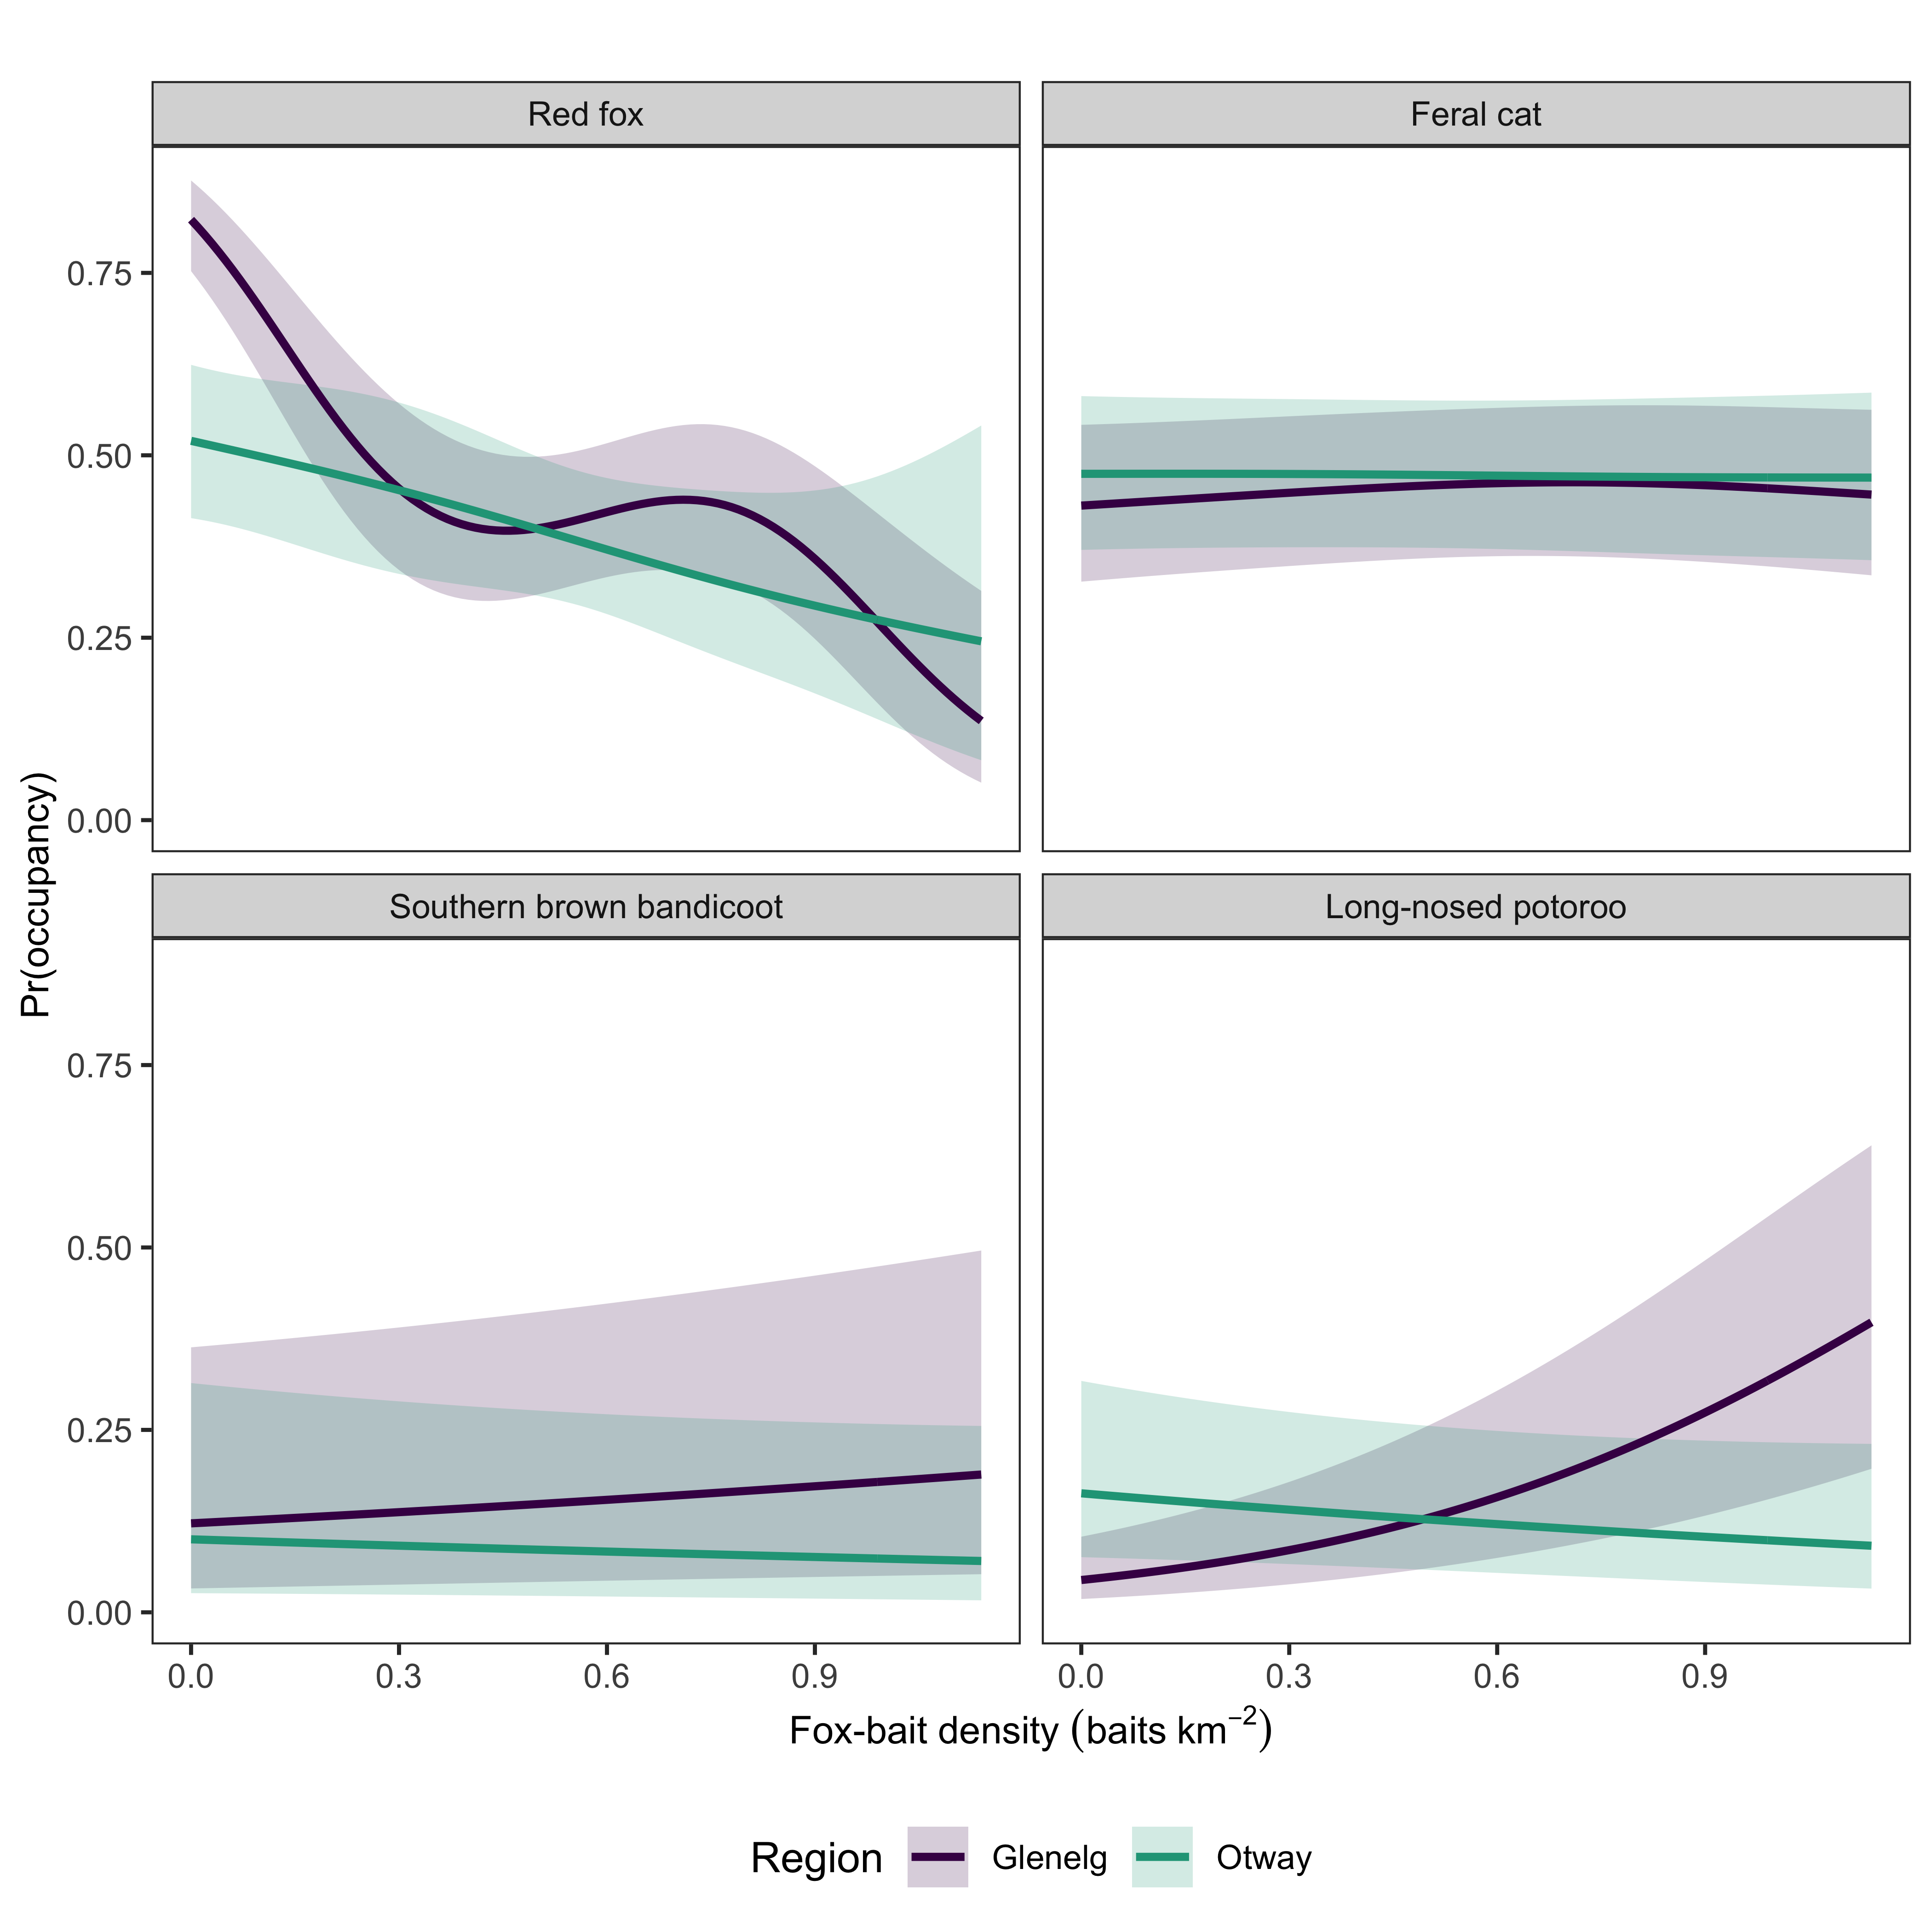
\includegraphics[width=1\linewidth]{figure/c1/foxbaits} 

}

\caption{Probability of fox occurrence (a) declined with increasing 1080 poison-bait density across both the Otway Ranges (blue) and Glenelg region (red) in south-west Victoria, Australia. Feral cat occurrence probability remain unchanged across the range of fox-bait density (b). Southern brown bandicoot (d) and long-nosed potoroo (e) occurrence probability increased with fox-bait density in the Glenelg region, but decreased in the Otway region--although these effects were weak with high uncertainty. Shaded regions indicate 95\% confidence intervals.}\label{fig:occ-1080}
\end{figure}
\newpage

\(~\)

\(~\)

\(~\)
\begin{figure}

{\centering 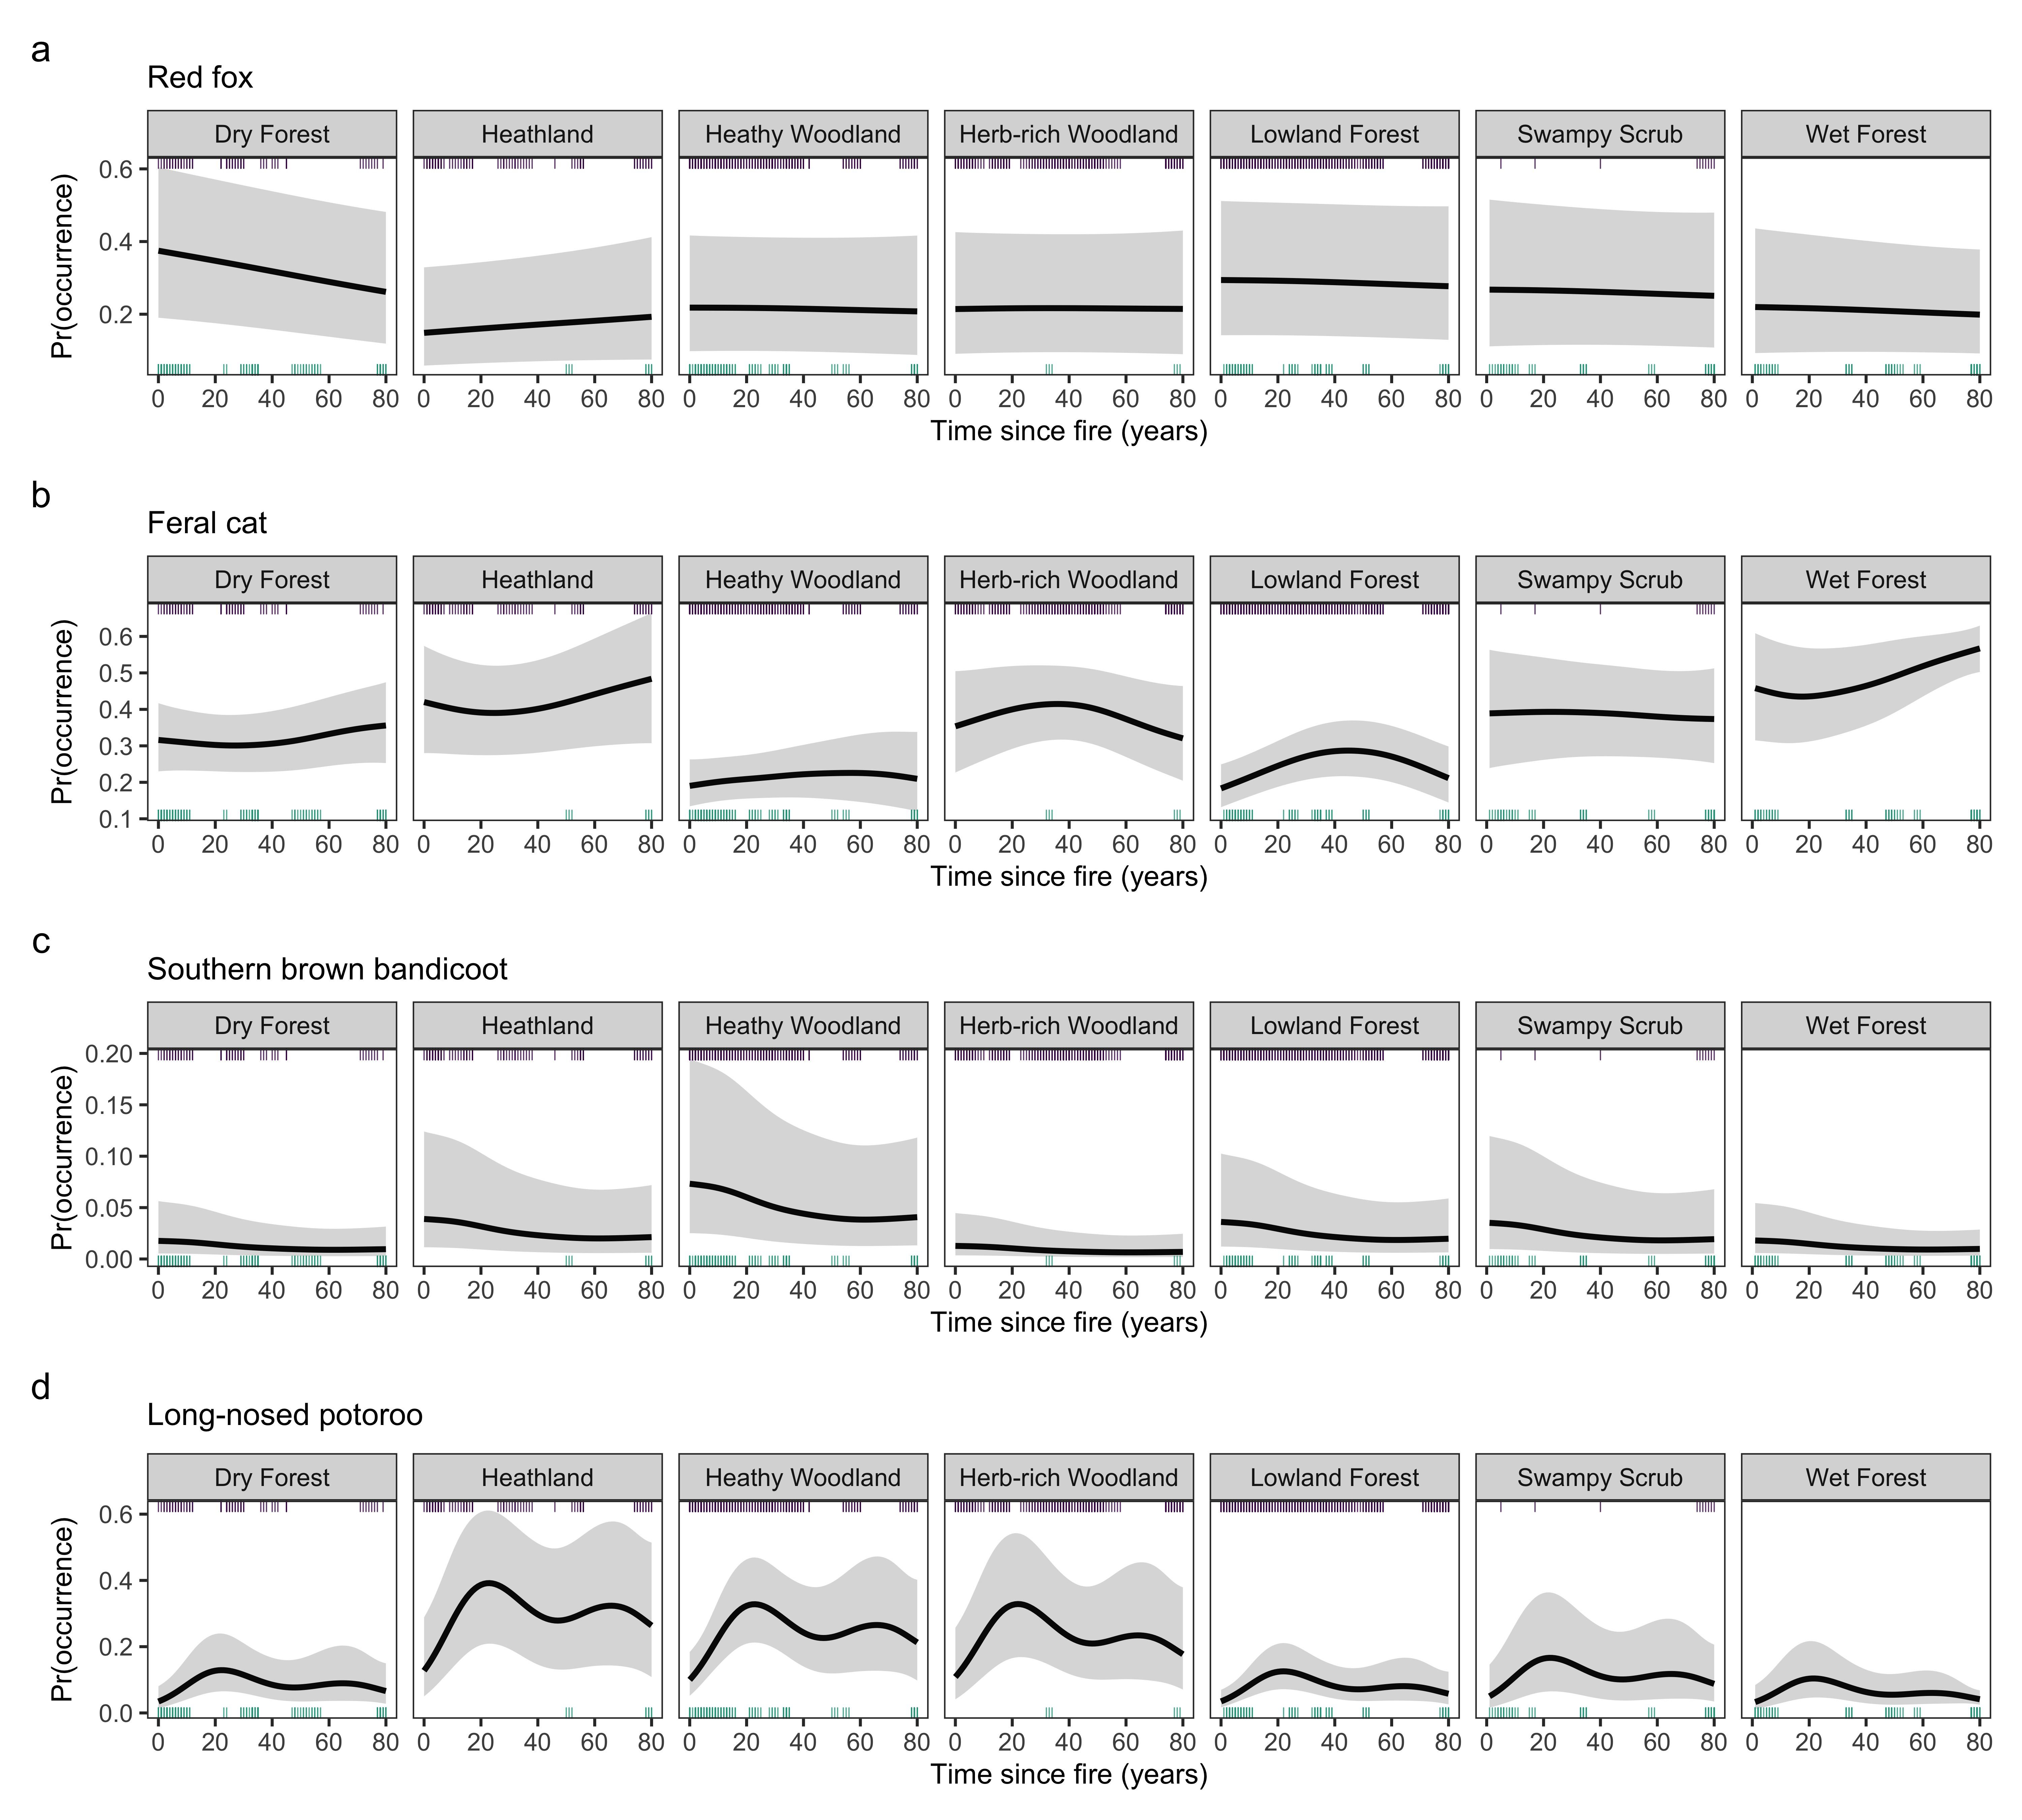
\includegraphics[width=1\linewidth]{figure/c1/tsf} 

}

\caption{Time since fire had a weak impact on fox (a) and feral cat (b) occurrence probability in south-west Victoria, Australia. Southern brown bandicoot occurrence probability (c) peaked around 15 and 75 years following fire, although, the magnitude of both peaks differed across Ecological Vegetation Class groups. Long-nosed potoroo occurrence probability (d) linearly increased with time since fire in heathy vegetation groups, but linearly decreased with years post-fire in Herb-Rich Woodlands. Shaded regions indicate 95\% confidence intervals}\label{fig:occ-tsf}
\end{figure}
\newpage

\(~\)

\(~\)

\(~\)
\begin{figure}

{\centering 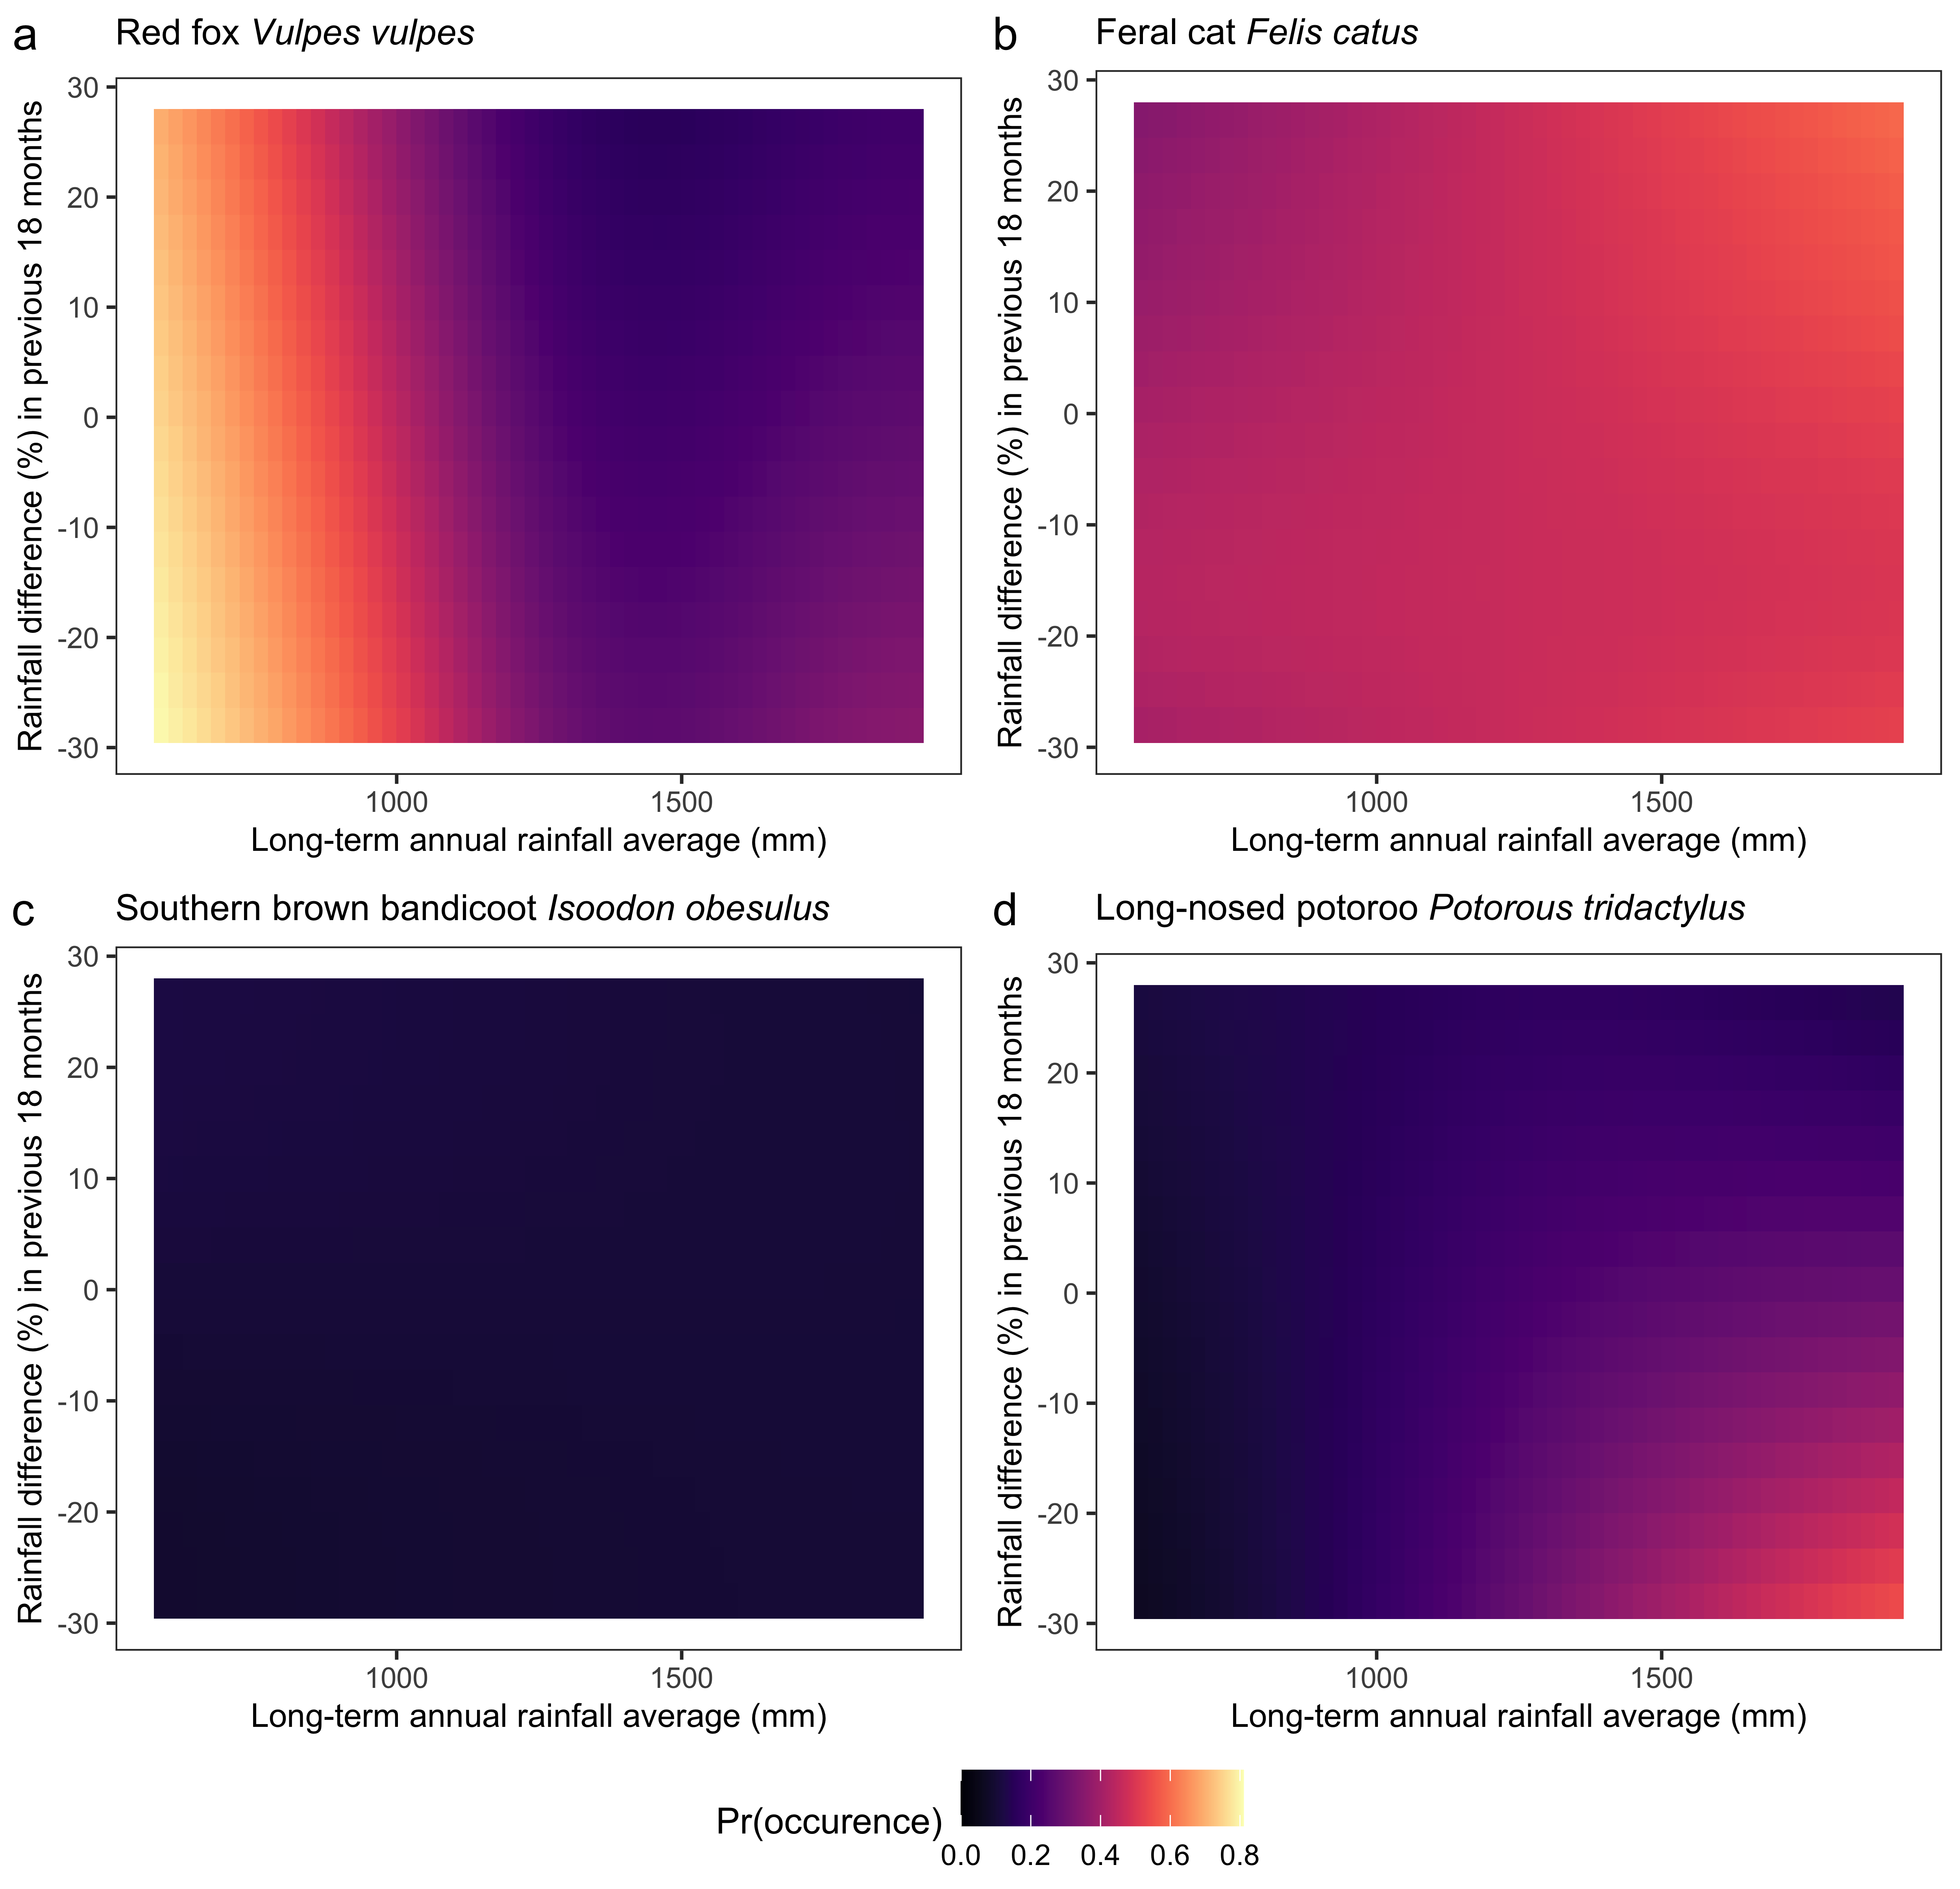
\includegraphics[width=1\linewidth]{figure/c1/rainfall} 

}

\caption{Impact of rainfall amount in the preceeding 18 months (percentage difference from the long-term median) on species' occurrence probabilities across the gradient of average annual rainfall (BIO12) in south-west Victoria, Australia. Fox occurrence probability was highest with low rainfall; strongly driven by changes in average rainfall across space, but only slightly impacted by temporal rainfall dynamics (a). Feral cat occurrence probability was highest where and when rainfall was highest (b). Rainfall patterns had no discernable impact on southern brown bandicoots (c). Long-nosed potoroo occurrence probability was highest at wetter sites during dry times (d). Shaded regions indicate 95\% confidence intervals}\label{fig:occ-rain}
\end{figure}
\newpage

\hypertarget{discussion}{%
\section{Discussion}\label{discussion}}

Here we demonstrate that large reductions in invasive apex predator occurrence don't produce consistent threatened species benefits. For example, a high density of 1080 poison-baits in the Glenelg region, Australia, largely maintains the persistence of LNP's in these landscapes, but appeared to slightly worsen outcomes for this threatened species in the neighbouring Otway Ranges. Fortunately, our work demonstrates that fox control is not the only effective tool mangers have--maintaining optimal fire regimes is a high priority for threatened native mammals in temperate landscapes. However, not only do optimal fire regimes vary across species, but they can be entirely conflicting for the same species across different vegetation communities. Our work highlights the importance of fine-scale monitoring and tailoring conservation strategies to local contexts.

Ours is the study first to quantify fox suppression across a gradient of 1080 poison-bait densities. Previous studies have not considered how baiting effort varies spatially when analysing the response of foxes and other species, rather averaging across the entire fox control program. There is a huge range in bait densities and replacement schedules for fox control across Australia. Compare to other studies and bait density recommendations.
The impact of poison-bait densities is relevant to the home-range size of the target species, which for foxes varies considerably (Main et al 2020) - caution needs to be taken when extrapolating to other sites. Ultimately, the best metric for fox control effectiveness is the improvement to native prey persistence.

Fox-bait density strongly correlated with fox suppression, however, the threatened species we surveyed had weak and inconsistent responses to fox-bait density. SBB's were mostly unaffected. Perhaps this is because bandicoots may more closely follow patterns in cat populations (Catling). On the other hand, LNP's (and other macropods) often benefit the most from fox control (hunter), but only did so in the Glenelg region. The most likely explanation for the lack of positive threatened species responses in the Otway Ranges were because we only surveyed for 0 - 3 years (relative to XX--XX years post-baiting in the Glenelg region) and did not account for time-lag effects. While these species have very short recruitment periods and so have the ability to respond quickly in terms of population density, we assumed that foxes are limiting the availability in suitable habitat for CWR mammals. Rather, we found that vegetation type and TSF were strong drivers of CWR mammal habitat suitability.

Contrary to the mesopredator release hypothesis, we observed no impact of fox control on cat occurrence probability. This may be because foxes do not suppress feral cat across these region, or because occurrence is too coarse a metric to uncover interactions between these species. Cats were widespread, and of all the species, had the lowest detectability, and the other explanatory variables relatively weak effects on their occurrence. Our occurrence models threw away rich information on detection rates, masking potential behavioural and population density effects.

Our work adds to the growing body of evidence that fire regimes are key to maintaining suitable habitat for small-medium sized native mammals. However, our study demonstrates that species response to fire can vary spatially. For local managers, preserving long unburnt heathy landscapes is a key management priority as they are strongholds for SBBs and LNPs. On the other hand, fresh burns in herb-rich woodland may promote LNP persistence. We saw weaker effects on the generalist invasive predators, contrary to some short-term experiments. This is unsurprising given our coarse, long-term (year) resolution, predator responses to fire and mostly finished within \textasciitilde3? months. Our result suggests that managers can focus on the heightened threat of invasive predators immediately post-fire (Hradsky refs) rather than over the long-term.

We observed surprising effects of rainfall on mammal occurrence. Feral cats were the exception, who's occurrence probability increased with both short and long-term rainfall. On the other hand, foxes, who had the strongest interaction with rainfall patterns, had higher occurrence probabilities with low rainfall. These responses may reflect different prey preferences. In a neighbouring region, Grampians, small mammals (rodent, antechinus) abundance followed short-term rainfall patterns - this increase in prey availability could explain cats occurring where rainfall is high. Foxes - I dunno? SBB's occurrence was not impacted by rainfall, LNP occurrence increased during dry periods within areas with high long-term rainfall averages. More effort is required to tease apart rainfall effects on mammal communities in these temperate landscapes. Directly quantifying time lag-effects with rainfall should be a future research priority, as should investigating interactive effects between species.

Invasive predators are well-documented to prefer forest edges, this was true for foxes but not for cats in our study. For foxes, this effect lasted for 2 km into the forest interior, but no effect was detected for cats. GAMs useful for quantifying this, rather than arbitrarily defining categorical edge habitat or assuming edge effects are linear. The weak and uncertain increase in CWR mammal occurrence with distance is intuitive because there is more habitat away from edges, and less foxes.

While increasing poison-bait density can suppress foxes, Australian threatened native mammals may not benefit unless habitat structure is maintained using careful fire regimes. Failure to account for these changing environmental conditions would have produced substantial noise around the fox control effect. Improved inference will likely come from comparing a range of population metrics, such as behaviour and density.
Invasive predators, fire, as well as changes to rainfall and fire regimes are pervasive biodiversity threats throughout the globe, including within protected areas. However, averaging effects across populations can be misleading because species responses vary.

\hypertarget{diel}{%
\chapter{Quantifying spatiotemporal shifts in predator behaviour across habitats, individuals and threats.}\label{diel}}

\hypertarget{abstract-1}{%
\section*{Abstract}\label{abstract-1}}
\addcontentsline{toc}{section}{Abstract}

\newpage

\hypertarget{introduction-1}{%
\section{Introduction}\label{introduction-1}}

Diel activity patterns - the distribution of activity throughout the daily cycle - are an important but overlooked aspect of behavioural ecology. Animals must allocate particular times of the day to rest, forage, socialise and reproduce, which are traded-off against threat avoidance (e.g.~predation) and deterrence against resource loss (i.e.~inter and intraspecific competition). Diel activity can therefore vary spatially across different environmental conditions (e.g.~food, shelter availability) and species assemblages. This is important to understand because constrained diel activity can incur fitness costs to individuals and populations (Lamb 2020 PNAS).

Flexible spatiotemporal behaviour can allow animals to adapt to changing conditions. For example, elk in Yellowstone National Park use risky, open parts of the landscape when the activity of reintroduced wolves is low, suggesting coexistence without major fitness costs (Kohl et al.~2019). Diel activity decisions are clearly linked to habitat type, and there is growing recognition of individual-level variation in these decisions (Basille et al 2015; time-limited seabirds; urban bears). Populations with high individual heterogeneity in diel behaviour are likely to be more adaptable to threats (Wolf and Weissing 2012; Dingemanse and Wolf 2013).

Diel activity patterns are increasingly being considered as technology like telemetry devices and camera-traps have become more widely available. Telemetry devices like GPS collars and accelerometers provide high resolution data at the individual-level. However, resource constraints generally limit these studies to few individuals (Harmsen 2009), which target personalities susceptible to physical capture. Camera-traps are particularly useful because they provide a more balanced view of the entire population and can detect multiple species, providing inference on ecological differences and species interactions. However, individual-level inference would be limited to species with unique markings. Distiller et al 2020 recently used camera-traps to individually identify jaguars and estimate sex difference in diel activity patters. Despite having information on individual diel activity patterns, studies predominantly estimate at the population-level due to small sample sizes. Most studies examine spatiotemporal behavioural responses by repeating spatial analyses at different time periods (predominantly night and day), but few consider continuous shifts in diel activity across spatial contexts.

A variety of statistical approaches are used to model continuous diel activity patterns, and examine how they vary among habitat types, individuals and co-occurring species. Kernel density estimation is most commonly used (Ridout \& Linkie 2009), despite being susceptible to noise from small sample sizes (Iannarilli \emph{et al.} 2019) and not incorporating explanatory variables (Frey \emph{et al.} 2017). Kernel density estimation remains popular because largely because they provide a coefficient which describes the estimated overlap between two diel curves. However, rarely are there only two interacting species or two categorical contexts for one species. To account for the spatiotemporal nature of species avoidance strategies, spatial overlap coefficients are increasingly being joined with temporal overlap coefficients (e.g.~Ait Kaci Azzou \emph{et al.} 2021; Farris \emph{et al.} 2020). However, a threat response may not be routine, but only employed or enhanced when the threat is heightened. Further, overlap coefficients may just reflect different niche preferences. Whether an animal \emph{changes} its activity patterns with an increasing threat level (e.g.~higher apex predator activity) is arguably more insightful and relevant to management than arbitrary overlap. Straightforward, integrated methods for examining changes in spatiotemporal animal behaviour are needed.

Generalised additive models (hereafter `GAMs') are increasingly used to estimate diel activity patterns. GAMs are essentially generalised linear models with added smoothing functions to allow nonlinear relationships between response and numeric explanatory variables (Wood 2017). The daily cycle can be binned into discrete intervals (e.g.~hour) and a smooth function of animal activity fitted using a cyclic cubic spline basis - where end points of the spline join (e.g.~last and first hour of the day). A maximum wiggliness is specified and complexity penalised (ultimately to a linear function) to avoid overfitting (unlike kernel density estimation). GAMs can incorporate interactions between explanatory variables (both categorical and numerical), however, there are few examples of this being used with diel smooths. This may because these features aren't widely known, or due to sample sizes being too small to fit a separate diel curves across different groups or contexts (e.g individuals, categorical environmental conditions). However, GAMs can be heirarchically specified to share information across categorical groups (Pedersen \emph{et al.} 2019). Hierarchical GAMs estimate an average response, as well as group-level estimates which are penalised as they deviate from the average - providing confidence that these are true deviations across groups.

Here we provide a case-study to illustrate how generalised additive models can be used to assess spatiotemporal behaviour of two predators. The red fox \emph{Vulpes vulpes} (hereafter `fox') and feral cat \emph{Felis catus} (hereafter `cat') have some of the widest distributions of any carnivores, and co-occur across most of their global range. Because of their devastating impacts on native prey in their introduced range, understanding differences in their behavioural ecology across space, and how foxes may impact feral cat behaviour is key to effective management. Numerous studies have investigated interactions between these invasive predators and environmental covariates, but not in a joint spatiotemporal modelling framework. We therefore investigated how predator activity varies across (1) space and (2) vegetation types, as well as (3) how fox spatial activity impacts cat diel behaviour and (4) individual heterogeneity in cats diel activity. We tested this in a simple predator system where only cats and foxes occur, and fox activity is manipulated through lethal control. This allowed sole focus on the interactions between these two predators, across an artificial gradient of apex predator (fox) activity.

\newpage

\hypertarget{methods-1}{%
\section{Methods}\label{methods-1}}

\hypertarget{study-area-1}{%
\subsection{Study area}\label{study-area-1}}

We collated camera-trap data across the Glenelg region and Otway Ranges in south-west Victoria, Australia (Fig. \ref{fig:diel-map}). The terrestrial mammalian predator guild is depauperate throughout both regions; native dingoes \emph{Canis familiaris} are long absent throughout, tiger quolls \emph{Dasyurus maculatus} are long-absent in the Glenelg region and likely functionally extinct in the Otway Ranges (last confirmed sighting in 2014 despite extensive camera-trapping). Introduced foxes and cats are therefore the only medium-large functional mammalian terrestrial predators across both regions. The purpose of each collated study was to experimentally survey changes in the mammalian community due to fox control. In broad sections of each region, government land managers conduct ongoing targeted fox control for biodiversity conservation. Poison baits containing 3 mg of sodium mono-fluroacetate (`1080') are buried at a depth of 10 cm at 1-km intervals along accessible forest tracks and roads. This allowed us to investigate fox-cat interactions across a gradient of apex predator (fox) activity and other landscape contexts. Prescribed fire is another key management action undertaken throughout both regions (except in very wet sections of Otway Ranges), primarily for asset protection.

In the Glenelg region, Gunditjmara country, natural vegetation--mostly lowland forests and heathy woodlands--is fragmented (Fig. \ref{fig:diel-map}). Foxes have been subject to lethal control in three distinct forest blocks (separated by pastoral farming and residential property) since October 2005, with 1080 poison-baits replaced fortnightly (Robley \emph{et al.} 2014a). Three similar, but unbaited, forest blocks to the north have been surveyed simultaneously as an experimental control (Robley \emph{et al.} 2014a).

The Otway Ranges, Gadubanud country, is a largely continuous patch of natural vegetation with a strong east-west rainfall gradient. A matrix of cool temperate rainforest and wet forest in the high-altitude south-west descends into a large heathland directly north, and into dry forests and then heathlands to the north-east. Foxes are controlled through 1080 poison-baits with monthly replacement across most of the Otway Ranges, but a large section to the north-west remains unbaited. The majority of this baiting began in 2016 - 2017, although fox-baiting commenced in some small sections in 2008.

\hypertarget{camera-trap-surveys-1}{%
\subsection{Camera-trap surveys}\label{camera-trap-surveys-1}}

We compiled camera-trap data from three distinct studies across the two regions; totalling 3667 deployments of camera-traps at 1232 camera-trap sites. Camera-traps were active for an average of 47 days, totalling 172,052 trapnights. Camera-trap spacing was variable; the average minimum distance between simultaneously deployed camera-traps was 445, 853 and 1266 metres for each study. Camera-traps were deployed in the Glenelg region between 2013 -- 2019, and in the Otway Ranges between 2016 -- 2019.

All camera-trap deployments consisted of a Reconyx (Holmen, Wisconsin) brand camera-trap (both white and infrared flash), attached to a tree or a metal picket, facing a lure. Camera-traps were set-up in two ways depending on the key aim of the project, either targeted toward predators or prey species. One study across both regions positioned camera-traps lower on a tree (around 15 - 30 cm above the ground -- angled only slightly downwards) facing a tuna oil lure approximately 2 - 2.5 m away (detailed in Rees \emph{et al.} 2019). The remaining camera-traps were positioned higher on a tree or a metal picket (at least 40 cm above ground) and angled downwards more strongly - facing a lure approximately 1 - 1.5 m away. These lures consisted of peanut butter, golden syrup and rolled oats mixed into a small ball, placed within a tea strainer or PVC pipe container and secured either to the ground, or 20 - 60 cm above ground on a wooden stake. All set-ups were effective in detecting both predator species.

\hypertarget{data-preparation}{%
\subsection{Data preparation}\label{data-preparation}}

We first created a table of species detections and deployment information (coordinates, dates) for every camera-trap deployment. All data analysis was conducted in R version 3.6.3 (R Core Team 2020). We used lorelograms to identify the minimum interval to approximate independence (Iannarilli \emph{et al.} 2019); this indicated discarding repeat detections of a species within 30 minutes was sufficient in reducing temporal autocorrelation. To account for day length variation across space and time, we extracted sunrise and sunset times for each camera-trap deployment using the `maptools' R-package (Bivand \& Lewin-Koh 2021) and adjusted detection times to be relative to sunrise and sunset using the average double anchoring approach described by Vazquez \emph{et al.} (2019). Using the `reshape' R-package (Wickham 2007), we manipulated the detection table into a dataframe with a row for each hour of the day, for every camera-trap deployment, recording the total number of `independent' fox and feral cat detections within each hour for the entire camera-trap survey duration.

We attached the Ecological Vegetation Class groups (``EVC''; DELWP 2020)) at each camera-trap location. Eight EVC groups types were surveyed in both regions, although to varying degrees (Table 1). In the Otway region, rainforests are finely interspersed (primarily in low lying gullies) throughout wet and damp forests, and so we merged these groups (hereafter `wet forests'). To account for fox control, we calculated the number of poison fox-baits within a 2.3 km radius around each camera-trap for each deployment - the average maximum distance foxes in these regions travel from their home range centre (Hradsky \emph{et al.} 2017). To investigate changes in feral cat diel activity in response to counts of foxes. We added an extra column to our dataframe with the total number of fox detections for each camera-trap deployment, divided by the log of the number of survey days to account for differences in camera-trap survey durations (hereafter `adjusted fox counts').

\hypertarget{generalised-additive-models}{%
\subsection{Generalised additive models}\label{generalised-additive-models}}

We modelled the total predator counts for each camera-trap deployment (response variable) with generalised additive mixed-effect models implemented in the `mgcv' R-package (Wood 2017). We used REML estimation and the negative binomial family (as overdispersion, but not zero-inflation, was detected using the `DHARMa' R-package Hartig (2020)). We specified a model offset to account for differences in camera-trap survey duration, and a random intercept for each site to account for repeat sampling. For fox models (n = 2), we included a smooth effect of poison-bait density using a thin plate regression spline basis. This formed the base model specification for each model we fitted. Models differed in their specification of the cyclical hour smooth in order to provide inference on variations of predator diel activity across (1) space (2) EVC groups, as well as for feral cats across the range of observed fox activity (3), and across each identified individual cat (4); detailed in the sections below. This model specification allowed both spatial activity to be higher in each context (i.e.~across coordinates, vegetation types, fox activity levels, individual cats) in addition to variable diel activity patterns. We plotted models using `ggplot2' and `gratia' R-packages (Wickham 2016; Simpson 2021).

\hypertarget{spatial-variation-in-predator-activity}{%
\subsubsection{Spatial variation in predator activity}\label{spatial-variation-in-predator-activity}}

We fit a model for each predator which included a tensor product interaction between a spatial smooth and hourly smooth. This allowed predators to have different activity levels across space (static across the years surveyed), as well as a variation in diel activity across space. Space was modelled using camera-trap coordinates and a duchon spline basis (Miller \& Wood 2014). To compare relative diel activity pattern strengths - how much activity patterns vary across the daily cycle - we plotted the difference between the minimum and maximum activity estimate for every predicted location.

\hypertarget{variation-in-predator-activity-across-vegetation-types}{%
\subsubsection{Variation in predator activity across vegetation types}\label{variation-in-predator-activity-across-vegetation-types}}

We estimated predator diel activity across EVC group using a hierarchical model specification; a global smoother for hour and group-level smoothers with shared wiggliness for the seven EVC groups (i.e.~model GS in Pedersen \emph{et al.} 2019). We included a random effect to account for overall differences between the two regions.

\hypertarget{feral-cat-spatiotemporal-avoidance-of-foxes}{%
\subsubsection{Feral cat spatiotemporal avoidance of foxes}\label{feral-cat-spatiotemporal-avoidance-of-foxes}}

Analysis of fox diel activity across EVC groups showed strong similarity between all vegetation groups except wet forests. We hypothesised that cats would temporally avoid foxes by becoming more diurnal in dry vegetation groups where foxes were mostly nocturnal, but not in wet forests where fox activity had little variation across the daily cycle. We therefore modelled fox-induced changes in feral cat diel activity separately for wet and dry vegetation groups. We further split dry vegetation groups by region for replication. We refer to the resulting variable as `habitat type', which had three levels: (1) wet forests and rainforests in the western Otway Ranges (`wet\_otways'), (2) dry EVC groups of the Otway Ranges (`dry\_otways') and the Glenelg region (`dry\_glenelg').

We used a tensor product of hour and adjusted fox counts smooths to model feral cat diel activity across the range of observed fox activity. We specified this with a by variable factor smooth to model separate responses for each habitat type. We modelled adjusted fox counts using a thin plate regression spline with shrinkage to penalise the null space in addition to the range space (i.e.~shrinking wiggly terms to linear functions) of the spline basis, meaning fox effects could be entirely removed from the model (while the hourly curves could be shrunk to a flat line due the inbuilt range space penalty; Marra \& Wood 2011). This model specification allows five different scenarios: that there was (1) no effect of hour or foxes on feral cats (2) a static hourly effect only, (3) a spatial response to foxes only, (4) a spatial response to foxes and an unrelated static hourly effect, (5) a spatial response to foxes and a hourly effect which changes across the range of fox counts. We also included a separate spatial smooth (using a duchon spline) to account for the effect of unmodelled environmental covariates (including overall differences in spatial activity between regions) and spatial autocorrelation.

\hypertarget{individual-variation-in-feral-cat-diel-activity}{%
\subsubsection{Individual variation in feral cat diel activity}\label{individual-variation-in-feral-cat-diel-activity}}

One of the collated datasets identified individual cats based on unique pelage patterns across the wet forests of the western Otway Ranges and four forest blocks in the Glenelg region (Chapter \ref{density}). We used only this dataset to model individual heterogeneity in cat diel activity using a hierarchical model specification. This included a global smoother which estimated the average diel activity for all detected cats (including unidentifiable cats), along with group-level smoothers for each identified individual, with a common wiggliness (i.e.~model GS in Pedersen \emph{et al.} 2019). This model structure penalises functions which deviate strongly from the average response; individual with few detections should take the shape of the global response.

\newpage
\begin{figure}

{\centering \includegraphics[width=1\linewidth]{figure/c4/fig1_map} 

}

\caption{Locations of our study regions in south-west Victoria, Australia. The grids of camera-traps are denoted by white dots. The Glenelg region is to the west and Otway region to the east. Native vegetation is indicated by dark green, with hill shading. \textit{Map tiles by Stamen Design, under CC BY 3.0, map data by OpenStreetMap, under CC BY SA.}}\label{fig:diel-map}
\end{figure}
\newpage

\hypertarget{results-1}{%
\section{Results}\label{results-1}}

Diel activity strength varied across space for both predators (Fig. \ref{fig:diel-space}). Foxes concentrated activity during particular times of the day, particularly in the Glenelg region, whereas feral cats had more consistent activity throughout the daily cycle. Both predators had similar spatial patterns in diel activity strength across space in the Glenelg region, but seemingly opposing patterns in the Otway Ranges. For example, fox diel activity strength was lowest in the wet forests of south-west Otway Ranges, where feral cat diel strength was highest, as was their overall level of spatial activity (Fig. \ref{fig:diel-veg}).

On average, both predators occupied similar times of the day--mostly nocturnal with activity peaks around sunrise and sunset (i.e., crepuscular; Fig. \ref{fig:diel-veg}i). The main difference was that fox activity peaked after sunset and they were less likely to be active during the day relative to cats. For foxes, little variation in this pattern was shown across all EVC groups except in wet forests--foxes were nearly as active during the day as they were at night in wet forests (Fig. \ref{fig:diel-veg}a). On the other hand, cats were nocturnal (and most abundant) in wet forests, but largely crepuscular in all other EVC groups (Fig. \ref{fig:diel-veg}b). Cats tended to be more active at sunset than sunrise. For both predator-vegetation models, the random effect for region (Glenelg or Otways) was shrunk to near-zero effect.

Across all habitat type replicates, feral cats changed diel patterns changed across the gradient of fox activity (Fig. \ref{fig:diel-cat-fox}). In the Glenelg region and dry Otway EVC groups, feral cats shifted from nocturnal-crepuscular diel patterns where fox activity was low, to being most active during the day where fox activity was high. In the wet forests of the Otway Ranges, feral cats became more strongly nocturnal with increasing fox activity. Cat spatial activity was relatively unaffected by the fox activity gradient in both habitat types of the Otway Ranges, but increased with the number of fox detections in the Glenelg region (Fig. \ref{fig:diel-cat-fox}).

There was high individual heterogeneity in cat diel activity patterns in the Glenelg region relative the wet forests of the Otway Ranges (Fig. \ref{fig:diel-individuals}). In the Glenelg region, the average diel activity pattern was shrunk to an almost flat line; diel activity curves were estimated nearly separately for each individual (individuals with few detections were heavily penalised towards a flat line). In the western Otway Ranges, feral cats on average were nocturnal; individuals mostly deviated with different activity peaks near sunrise and sunset times or the strength of diel activity (i.e., difference between high and low activity throughout the daily cycle). We had data from 39 individual cats in the Glenelg region and 94 individuals in the western Otway Ranges.

Overall, we collated 5449 and 2202 `independent' (separated by at least 30 minutes) detections of foxes and cats, respectively (Table \ref{tab:diel-tab1}. The models explained 18.1 - 35.2\% of null deviance (n = 7). Cat models with individual variation had relatively poor model fit (based on adjusted r-square values).

\newpage

\begingroup\fontsize{10}{12}\selectfont
\begin{longtable}[t]{llrrrr}
\caption{\label{tab:diel-tab1}Summary of the number of camera-trap deployments, unique survey sites and 'independent' counts of invasive predator detections across Ecological Vegetation Class groups within the Glenelg and Otway regions, south-west Victoria, Australia.}\\
\toprule
Vegetation & Region & Sites & Deployments & Fox counts & Cat counts\\
\midrule
Dry Forest & Glenelg & 25 & 69 & 347 & 9\\
 & Otway & 111 & 314 & 341 & 158\\
Heathland & Glenelg & 40 & 119 & 265 & 59\\
 & Otway & 3 & 9 & 8 & 6\\
Heathy Woodland & Glenelg & 154 & 424 & 574 & 96\\
\addlinespace
 & Otway & 82 & 256 & 160 & 66\\
Herb-rich Woodland & Glenelg & 59 & 373 & 863 & 198\\
 & Otway & 2 & 6 & 3 & 2\\
Lowland Forest & Glenelg & 383 & 1046 & 1900 & 290\\
 & Otway & 52 & 163 & 190 & 35\\
\addlinespace
Swampy Scrub & Glenelg & 4 & 10 & 19 & 8\\
 & Otway & 36 & 98 & 64 & 88\\
Wet Forest & Otway & 281 & 780 & 715 & 1187\\
\bottomrule
\end{longtable}
\endgroup{}

\newpage
\begin{figure}

{\centering 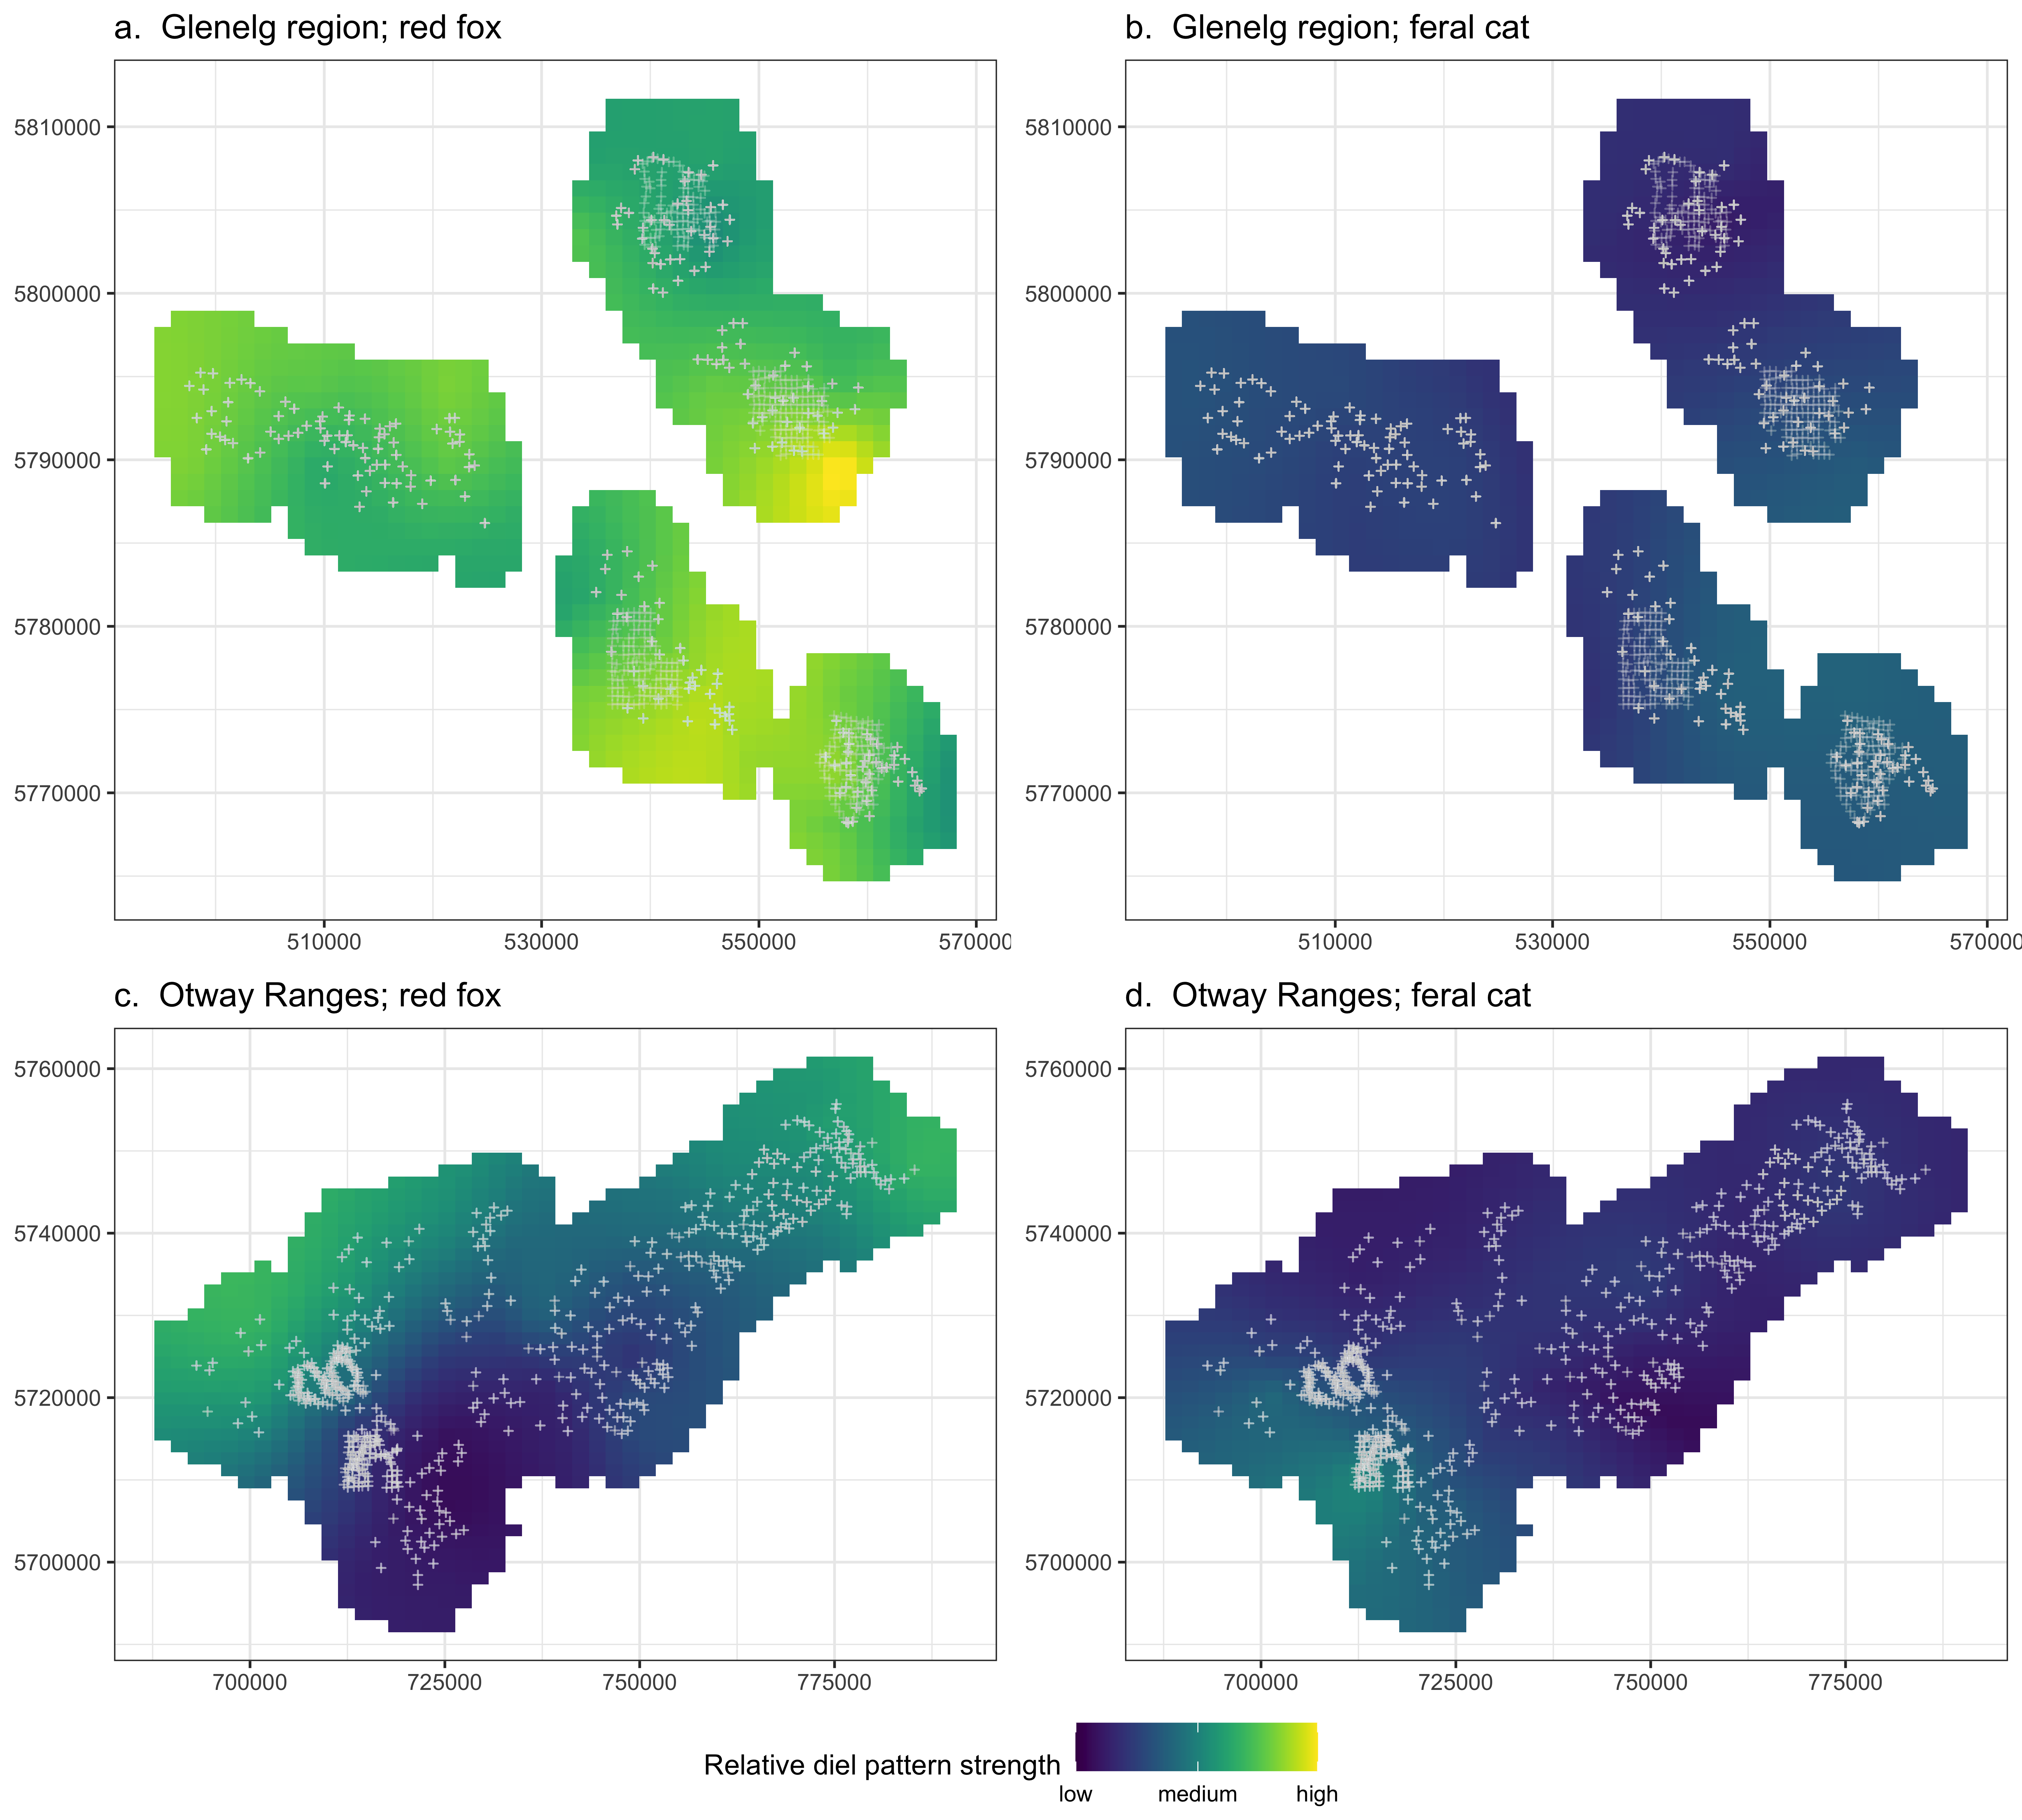
\includegraphics[width=1\linewidth]{figure/c4/diel_strength_600dpi} 

}

\caption{Relative spatial patterns of invasive predator diel activity strength across the two study regions in south-west Victoria, Australia. White crosses depict unique camera-trap sites; colour brightness scales with increasing difference between the minimum and maximum activity estimate over the 24-hour cycle for each location. Red foxes \textit{Vulpes vulpes} concentrate their activity during particular times of the day--especially in the Glenelg region (a)--whereas feral cats \textit{Felis catus} have a relatively consistent activity throughout the daily cycle. Both predators exhibited similar spatial patterns in diel activity strength across the Glenelg region, but seemingly opposing patterns in the Otway Ranges.}\label{fig:diel-space}
\end{figure}
\newpage
\begin{figure}

{\centering 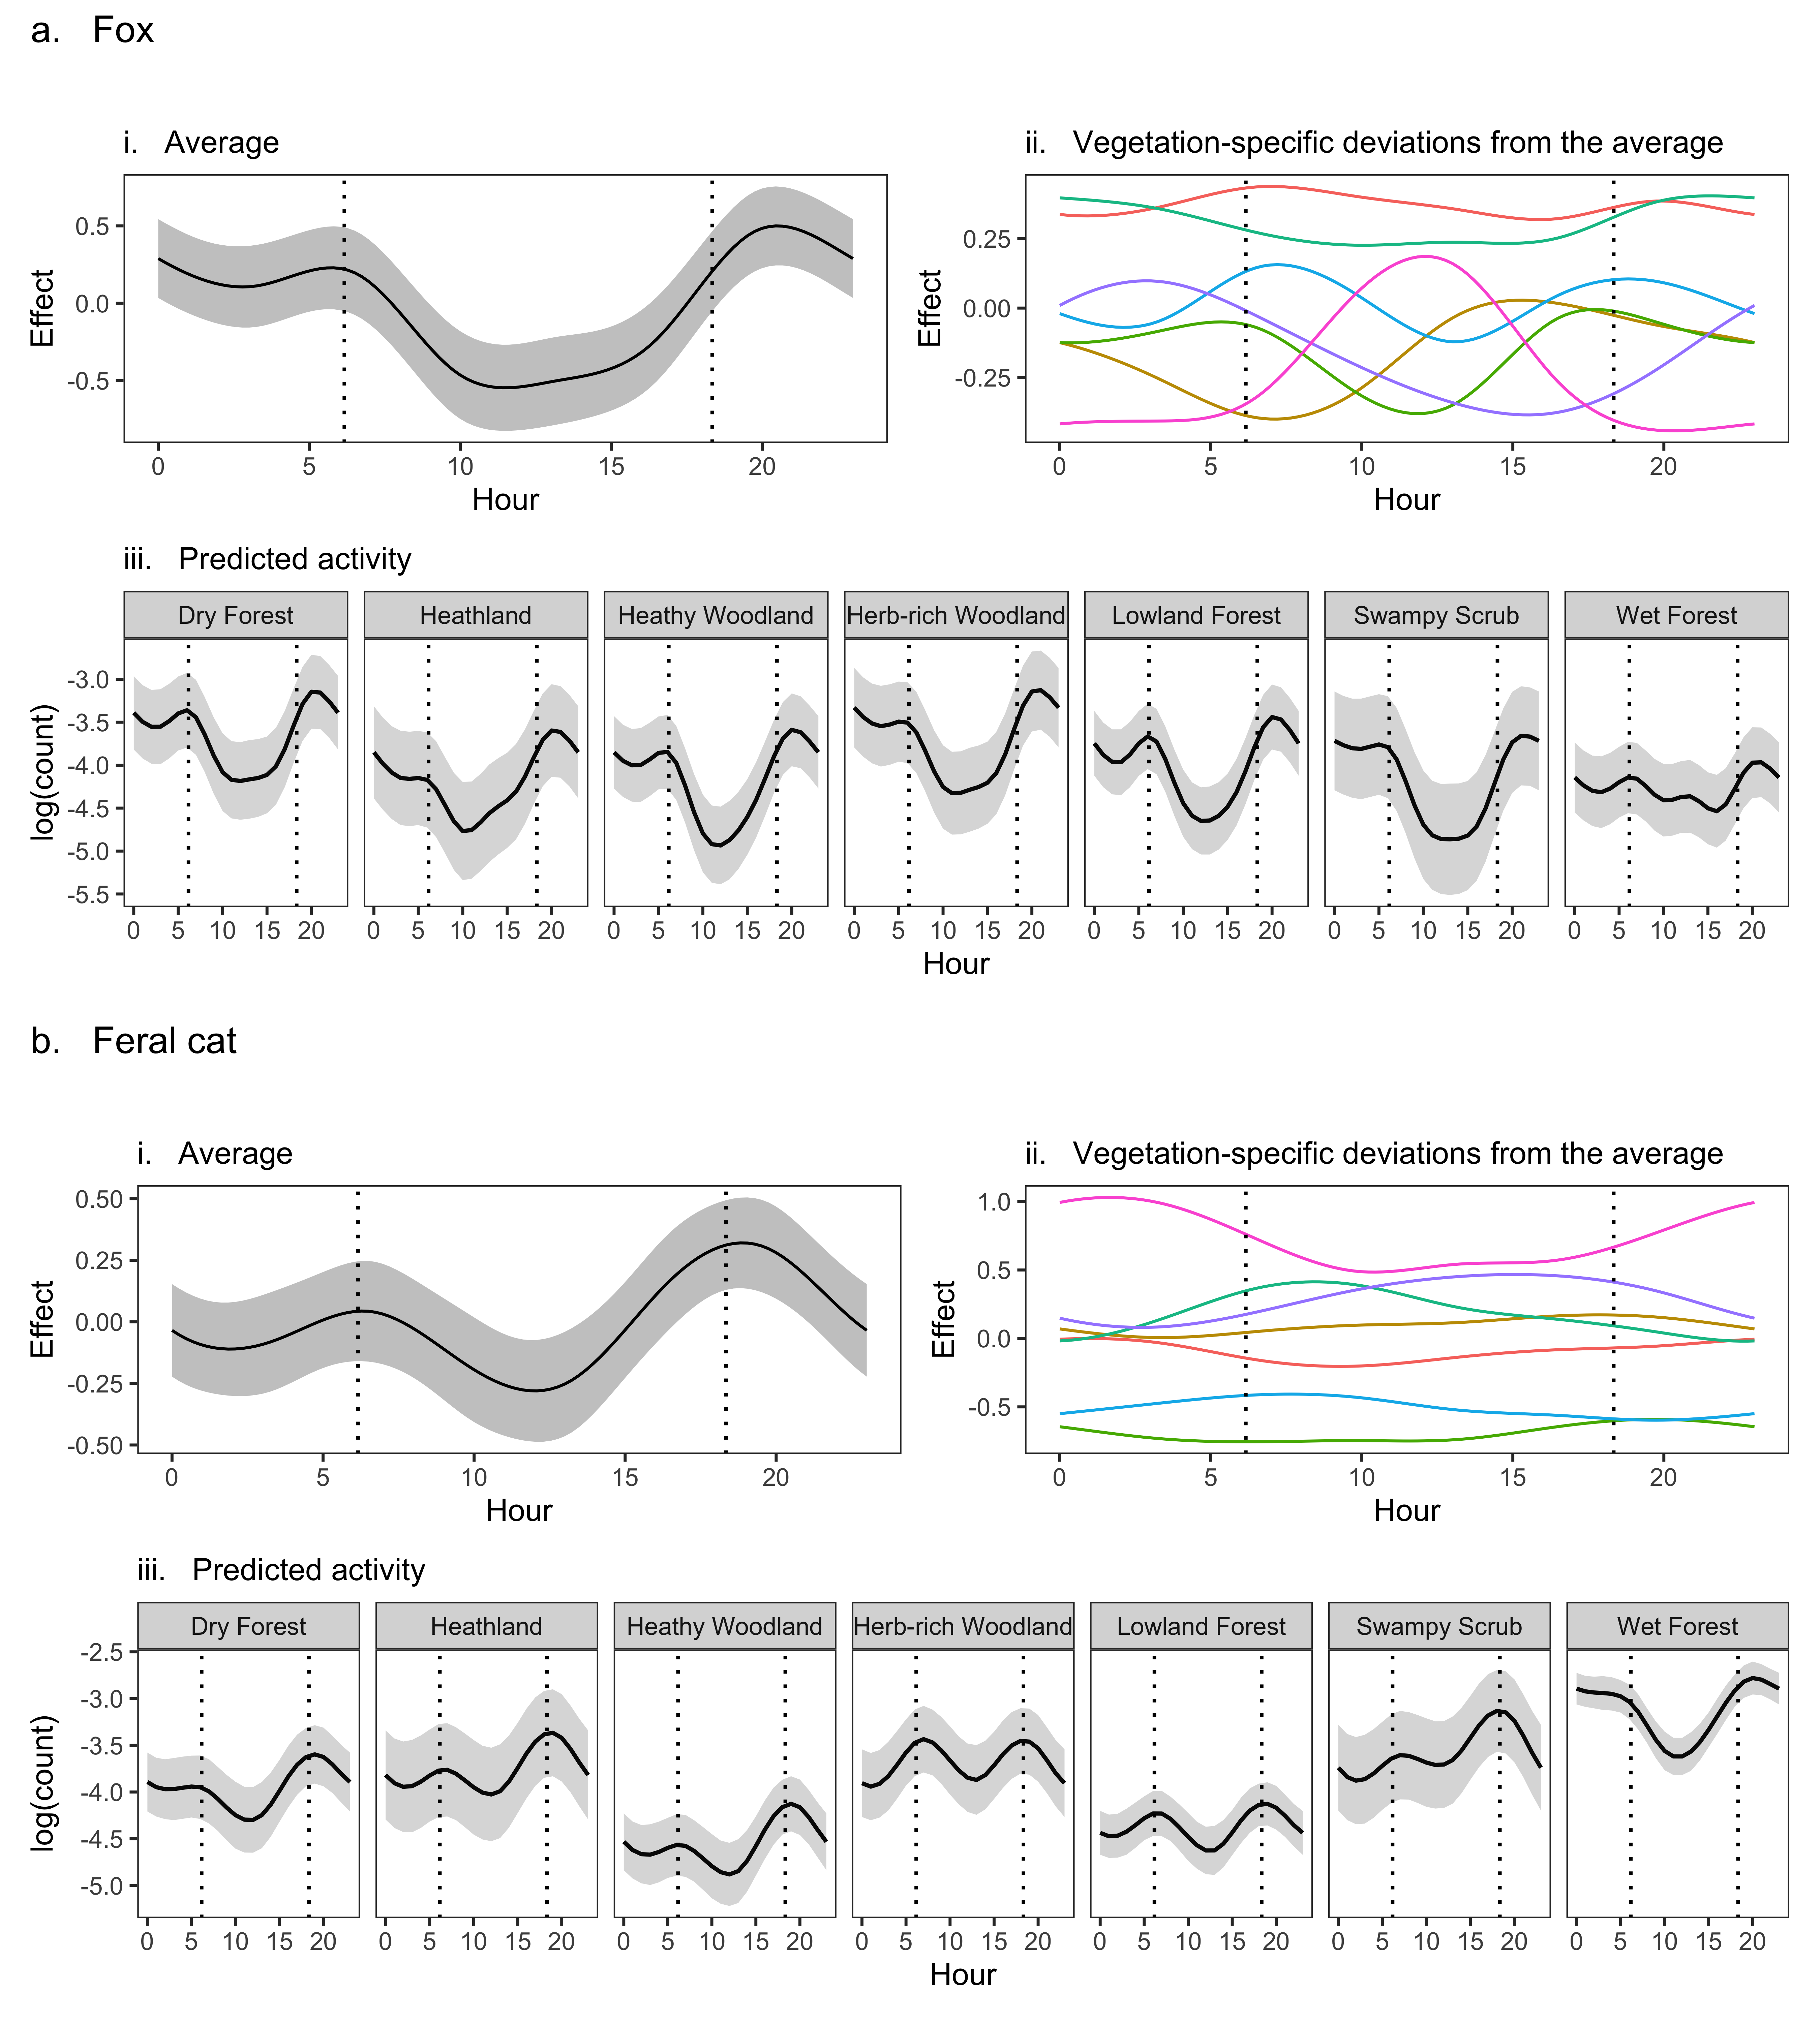
\includegraphics[width=1\linewidth]{figure/c4/predator_veg} 

}

\caption{Red foxes \textit{Vulpes vulpes} (a) and feral cat \textit{Felis catus} (B) activity patterns across Ecological Vegetation Class (EVC) groups in south-west Victoria, Australia. Dotted, vertical lines represent average sunrise and sunset times. Shaded areas indicate 95\% confidence intervals. Both invasive predator have an average (i) crepuscular - nocturnal diel activity pattern, with slight deviations across the dry EVC groups and larger deviations in wet forests. Unlike feral cats, fox spatial activity was relatively consistent across EVC groups.}\label{fig:diel-veg}
\end{figure}
\newpage
\begin{figure}

{\centering 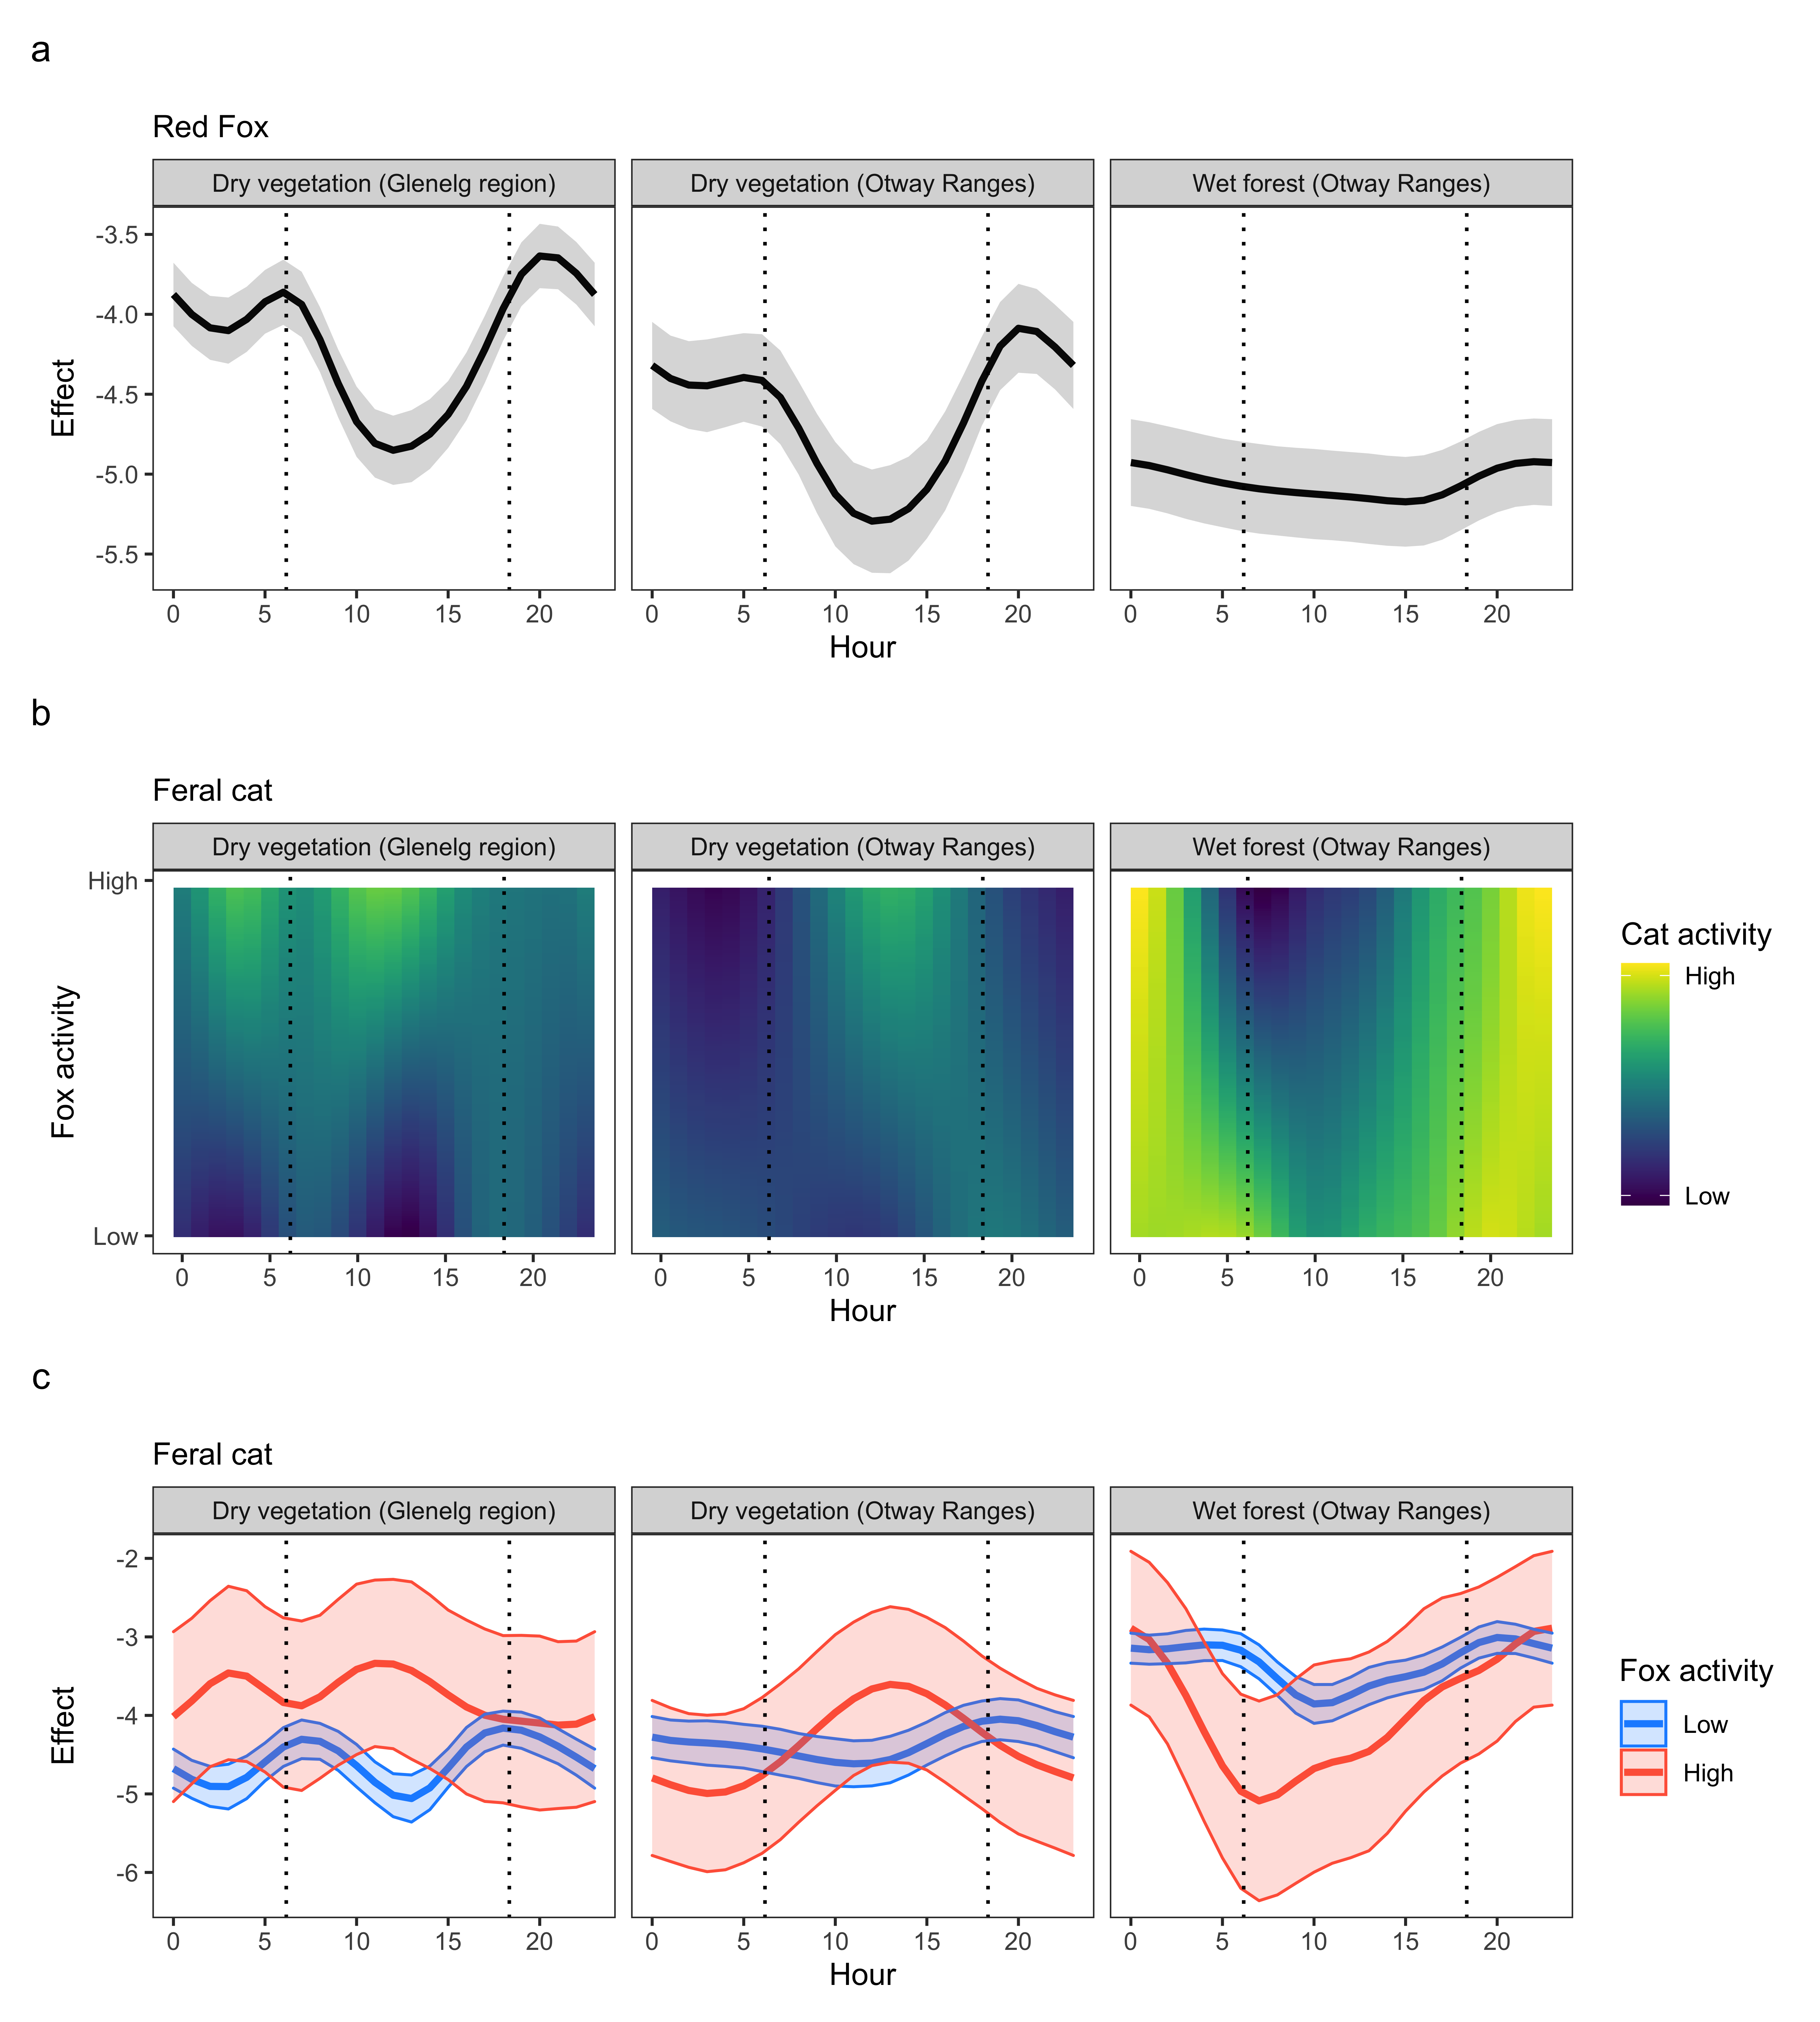
\includegraphics[width=1\linewidth]{figure/c4/cat_fox_count} 

}

\caption{Variation in feral cat \textit{Felis catus} activity (a) and uncertainty (b) in response to 'independent' red fox \textit{Vulpes vulpes} detections (log-transformed and survey effort adjusted) across each 'habitat type' in south-west Victoria, Australia. Grey vertical lines respresent average sunrise and sunset times. In the Glenelg region, there were more feral cat detections where there were more fox detections, but diel activity shifted from night to day (a). In the Otway Ranges, feral cats shifted to diurnal activity where fox actity was high in dry vegetation types (b), but became more nocturnal where fox actity was high in the rainforests and wet forests (c).}\label{fig:diel-cat-fox}
\end{figure}
\newpage
\begin{figure}

{\centering 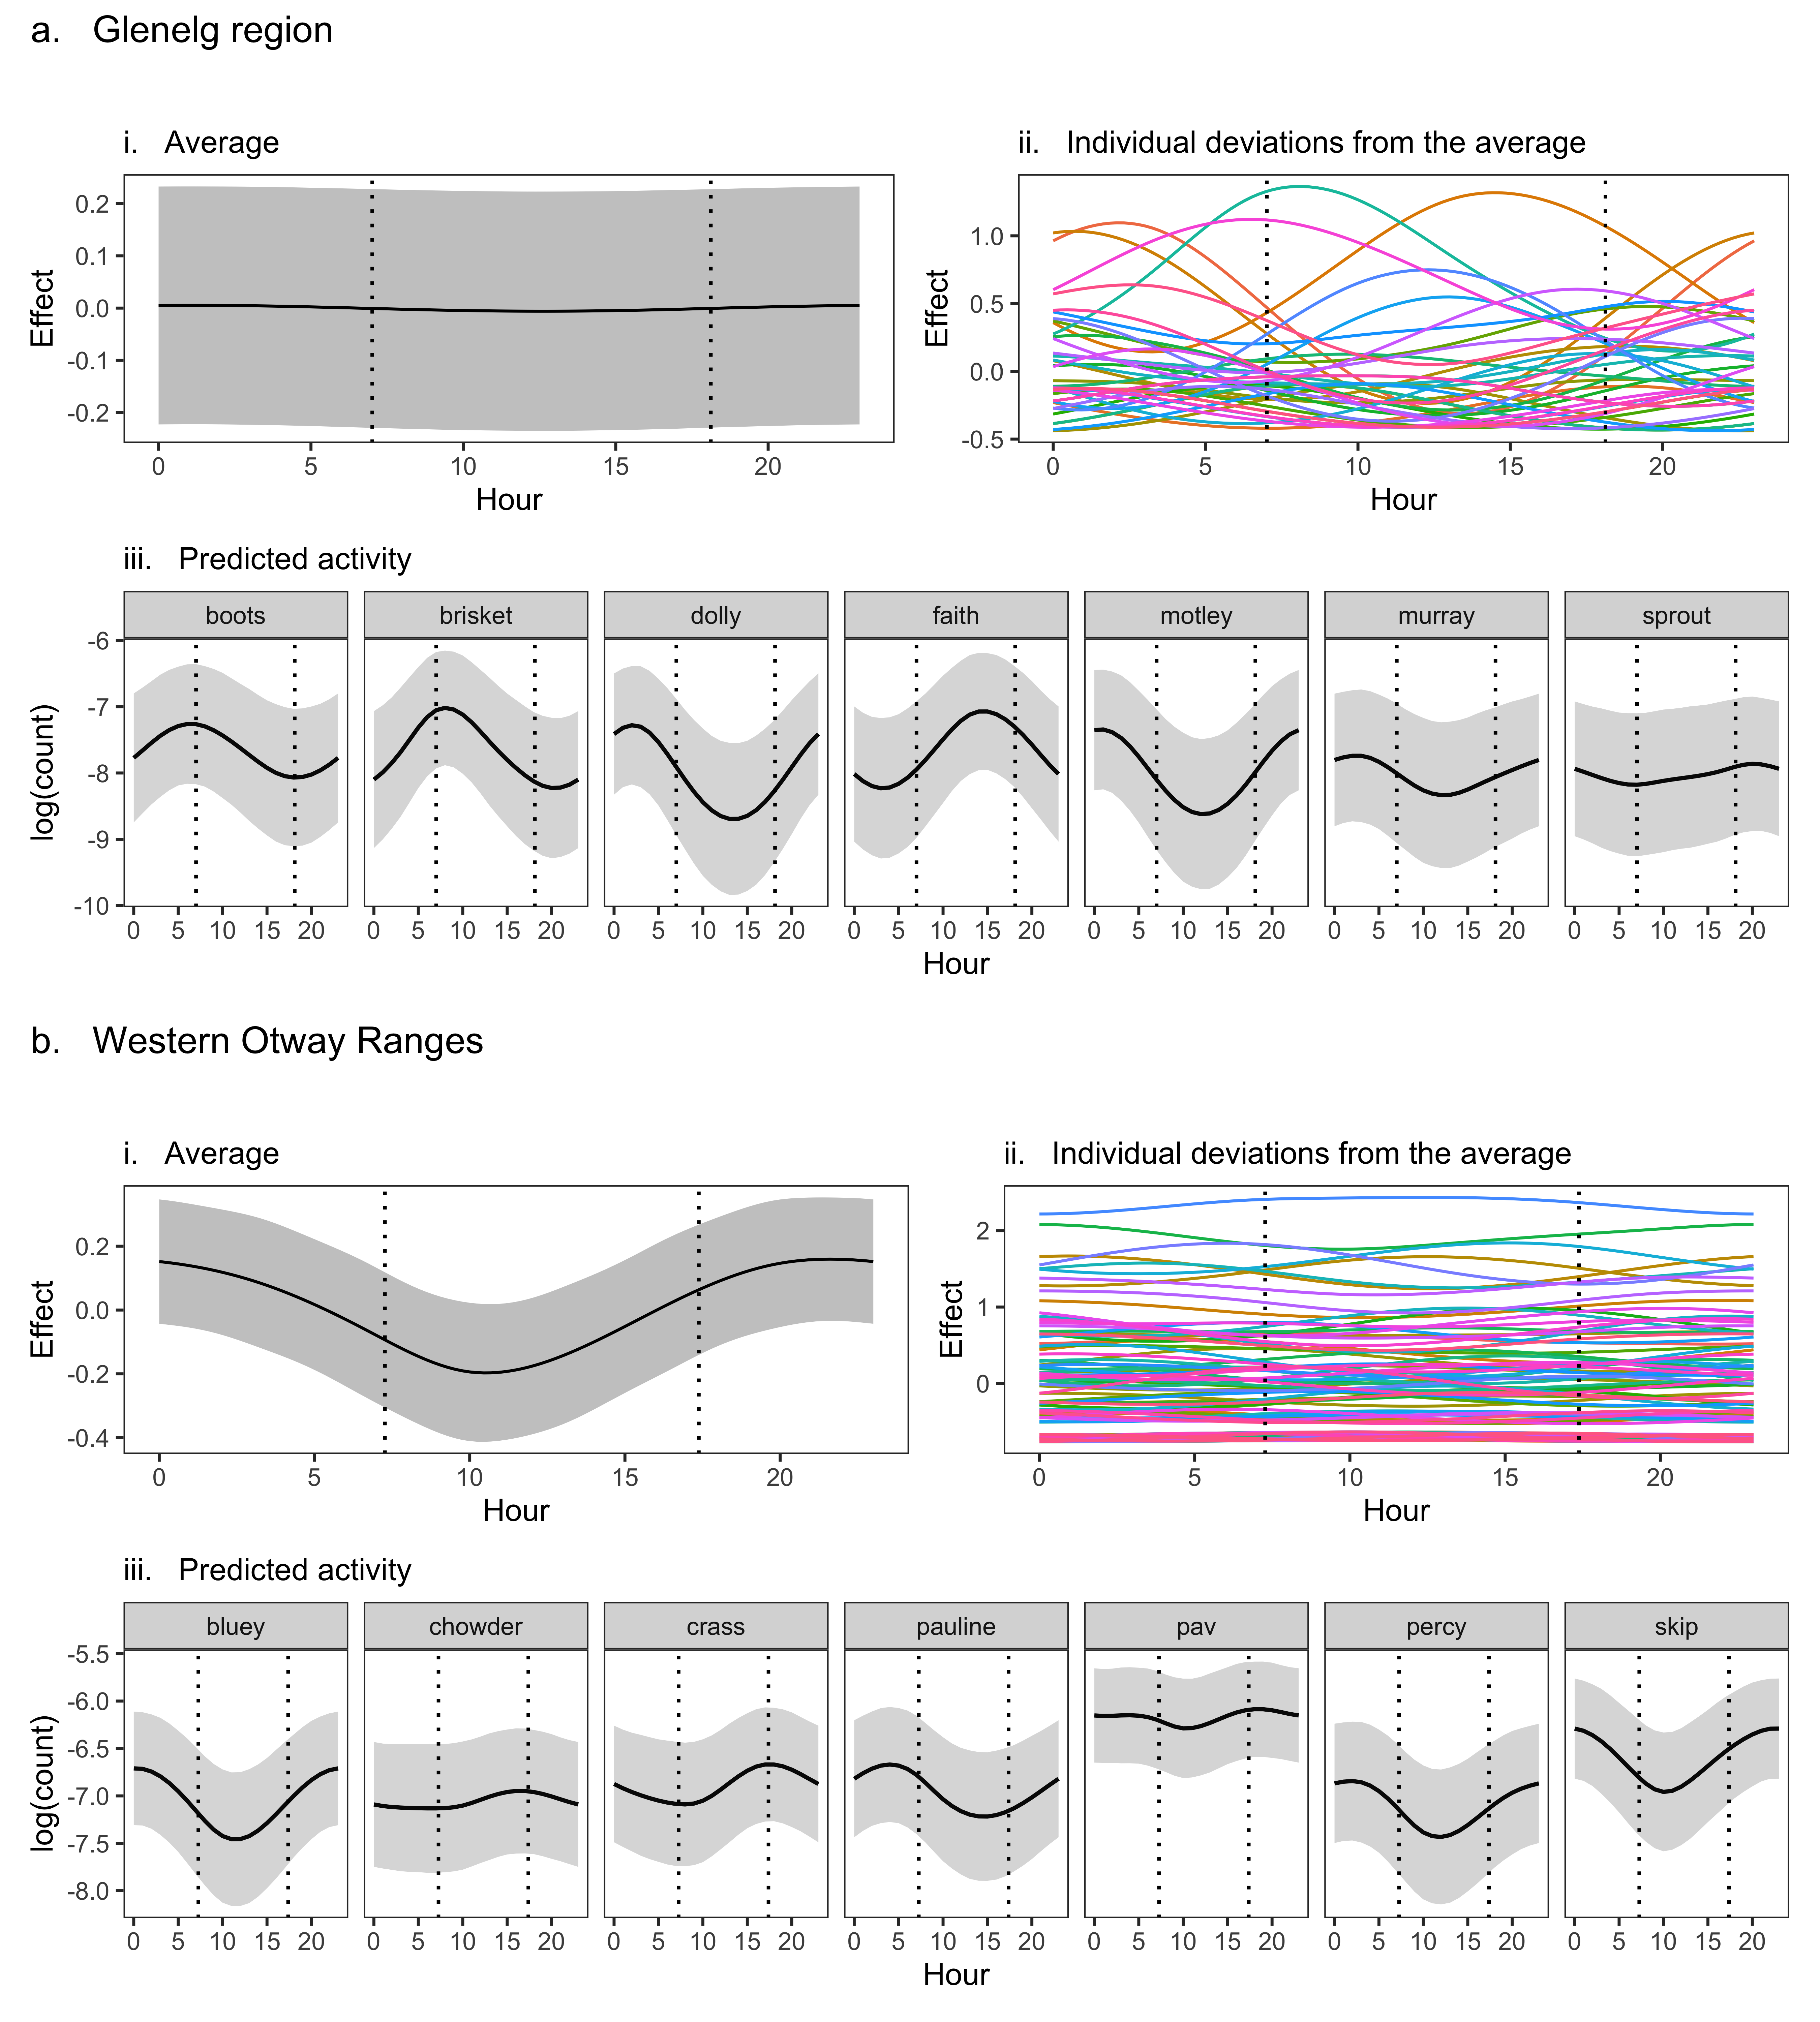
\includegraphics[width=1\linewidth]{figure/c4/cat_ind} 

}

\caption{Individual heterogeneity in feral cat \textit{Felis catus} diel activity across the Glenelg region (39 identified individuals; a) and wet forests of the western Otway Ranges (94 identified individuals; b) in south-west Victoria, Australia. As an example, the predicted activity of the seven individuals with the most detections (iii). Dotted, vertical lines represent average sunrise and sunset times. Shaded areas indicate 95\% confidence intervals. The global function of feral cat diel activity in the Glenelg region was shrunk to an almost flat line, signalling high individual variation (deviations can therefore be interpreted directly as unique diel patterns). In the Otway wet forests, feral cats were on average nocturnal, individuals mostly deviated with different activity peaks near sunrise and sunset times.}\label{fig:diel-individuals}
\end{figure}
\newpage

\hypertarget{discussion-1}{%
\section{Discussion}\label{discussion-1}}

Animal diel activity patterns are usually averaged across populations and regions, but here we have demonstrated just how variable diel patterns are across individuals, threat-levels and landscape contexts. Understanding how diel activity varies across different habitats provides important context for exploring threat avoidance responses. We found that foxes were likely a strong driver of feral cat diel activity across three replicates -- able to completely shift cat activity from night to day. Diel activity patterns are complex--GAMs offer a robust, flexible way to model diel activity across different circumstances.

Foxes tended to strongly concentrate activity during particular times of the day, but this varied substantially across space. In these study regions, Hradsky found half her GPS collared spent the night travelling to farm / townships, and days in the forest. Proximity to forest edge would be worth exploring the future. Strongest fox diel strength variation was seen in the Otways, here it appeared closely tied to vegetation type: heathland (strongest), dry forest (moderate), and wet forest (weakest). This was confirmed by our vegetation analysis. Perhaps this is due to differences in prey availability or exposure / shelter availability (e.g.~eagles, humans) or thermoregulation? However, foxes and cats share a similar niche / lots of prey - and had different activity patterns across veg types - so this is unlikely to be driven purely by environmental constraints. Cats had similar spatial patterns in diel strength to foxes in glenelg, but seemingly opposite in the Otways - perhaps avoidance.

Both predator species had extremely similar diel activity patterns on average, however, subordinate cats shifted activity to less risky times of the day as apex predator (fox) activity increased. We observed these shifts in diel activity with increasing threat levels across our three replicates. Where foxes were largely nocturnal (dry vegetation types) cats increased activity during the day across in the Glenelg and Otway regions. Where foxes were active consistently throughout the daily cycle, cats concentrated activity around midnight (Fig. \ref{fig:diel-cat-fox}). This likely reflects temporal avoidance, and demonstrates that avoidance can be dynamic across different contexts. Cats are expected to avoid foxes spatially, however, we observed no spatial association between cats and foxes in the Otways, and a positive correlation between the predators in the Glenelg region. Cats and foxes have similar requirements, and so, shifting diel activity patterns perhaps allows spatial coexistence in the Glenelg region. This result demonstrates the importance of modelling changes in predator diel activity, not just overlap, and considering this in a joint spatiotemporal framework.

One question which arises from this work is whether individuals themselves have flexible diel patterns, or is individual variation due to the unique spatial context of an animals home range? Cats in the Glenelg region had more variation in diel activity than similarity; Otway cats broadly followed an average nocturnal pattern with small deviations. Perhaps this was because individual cats were identified across a large area in the Glenelg region, whereas where we surveyed cats across a much smaller, and more heterogenous in terms of vegetation type. Fox activity was also lowest here (western Otway wet forests), with weak diel activity patterns meaning cats could avoid foxes just as easily at night compared to day, unlike Glenelg. We therefore expect the higher diel activity variation across individuals cats the Glenelg region to reflect the higher variation in habitats and threats from foxes which require more drastic changes. To better test this, a future research priority, would be to model diel activity patterns shifts within individuals (e.g.~refs). Although this would require more intensive data.

We are not aware of other approaches which have used heirachical or spatial models of diel activity. The only other approach we have seen was to model diel activity with continuous covariates is Cunningham. Differences: - quasibinomial, not spatiotemporal. Linear correlation with spatial apex predator abundance - We used a tensor product which included a smooth of apex predator counts because predator interactions may not be linear ({\textbf{???}}). This also, allowed us to combine with shrinkage - so this association between the species could be completely removed if the data didn't support such an interaction. Combined spatiotemporal modelling - differences to other approaches.

Our GAM approaches is simple and flexible. Robust - more aligned with null hypothesis testing - small sample sizes shrink to a flat line (or to the average), in contrast to circular overlap which produces spurious shapes. Small sample sizes are usually a problem. Studies often condense grouping categories without testing. We demonstrate hierarchical model specification to share information - ability to pool all available data - easily adapted to other contexts. Limitation: hour is an explanatory - not response variable. Our purpose was inference, so running multiple models not an issue. But for prediction, it would be nice to have multiple variables impacting hour at the same time. Does not (clearly) separate numerical responses from behavioural, see Borchers SCR paper for a possible avenue for this.

Without modelling changes in diel activity, we would have, like many others, inferred no impact of foxes on cats. Invasive predators are useful species to test this on, as they are extremely adaptable to different conditions. Predator diel activity patterns strength and individual varied considerably between the two regions - cautioning extrapolation of behavioural patterns for these widespread, generalist predators to other areas. Implications for prey.

\hypertarget{otways17}{%
\chapter{Unexpectedly high densities of feral cats in a rugged temperate forest}\label{otways17}}

\hypertarget{abstract-2}{%
\section*{Abstract}\label{abstract-2}}
\addcontentsline{toc}{section}{Abstract}

Effective invasive predator management requires accurate knowledge of population density. However, density can be difficult to estimate for wide-ranging, cryptic and trap-shy species, such as the feral cat \emph{Felis catus}. Consequently, few density estimates exist for this invasive predator of global significance, particularly from rugged, mesic or structurally complex habitats where detection is challenging. In this study, we estimated feral cat density in the wet forests and cool temperate rainforests of the Otway Ranges, south-eastern Australia, to (1) provide a density estimate for this rarely surveyed habitat type, and (2) verify predictions from a continental-scale model of feral cat density. We deployed 140 camera traps across two independent 49 km\textsuperscript{2} grids and identified individual feral cats based on unique pelage markings. Using spatially explicit mark-resight models, we estimated that there were 1.14 cats km\textsuperscript{-2} (95\% CI: 0.88 -- 1.47). This is more than three times the average cat density in natural environments across Australia, and at least five times higher than model-based predictions for the Otway Ranges. Such high densities of feral cats likely reflect the abundance of small native mammals and lack of apex predators in our study area. Our findings contradict the widespread assumption that feral cats occur at very low densities in mesic and rugged habitats. Underestimating the density of feral cats in these environments has significant implications for pest animal management and biodiversity conservation.

\newpage

\hypertarget{introduction-2}{%
\section{Introduction}\label{introduction-2}}

Accurate estimates of the distribution and abundance of invasive predators are essential to determine ecosystem impacts, inform effective management and target control efforts. However, this information is difficult to obtain as predators are often cryptic, trap-shy and occur at low densities (Royle \emph{et al.} 2008). A prominent example is the feral cat \emph{Felis catus}, which is implicated in the extinction or decline of 430 species globally (Doherty \emph{et al.} 2017). A better understanding of feral cat density has been highlighted as a priority for effective management of both this species and its threatened native prey (Woinarski \emph{et al.} 2014; Legge \emph{et al.} 2017; Moseby \emph{et al.} 2019).

Legge \emph{et al.} (2017) developed a continental-scale model of feral cat density for Australia which has had considerable implications for feral cat research and management. For instance, the model has been used to estimate the number of birds, reptiles and mammals killed annually across Australia by feral cats (Woinarski \emph{et al.} 2017, 2018; Murphy \emph{et al.} 2019). As the model estimated that there were considerably fewer feral cats in Australia than previously expected, it also casts doubt on the feasibility of Australian Federal Government's plan to cull two million feral cats between 2015 and 2020 (Doherty \emph{et al.} 2019). Given the importance of feral cat density estimates for policy, planning and management, it is vital to verify and refine the model's predictions.

The underlying data used by Legge \emph{et al.} (2017) had several limitations, including that feral cat density estimates were not available for any wetland, mangrove, dense heath or rainforest environments in Australia (Legge \emph{et al.} 2017). This likely reflects the difficulty of access and ineffectiveness of traditional feral cat monitoring methods (track counts and spotlight counts) in these structurally complex habitats (Denny \& Dickman 2010). Legge \emph{et al.} (2017) highlighted the need for more site-based density surveys, particularly in these under-studied environments. Further, nearly all of the density estimates collated by Legge \emph{et al.} (2017) were based on studies that did not identify individual cats or account for imperfect detection (i.e.~the possibility that some individuals were not detected). Such methods can be unreliable when inferring across sites, times, ecological contexts and different detection methods (Edwards \emph{et al.} 2000; Hayward \emph{et al.} 2015), particularly for species such as cats whose densities may fluctuate substantially over time in some regions (Legge \emph{et al.} 2017). Concurrent surveys of cats on Kangaroo Island and the adjacent Australian mainland suggests that the Legge \emph{et al.} (2017) model may substantially underestimate this variation in density (Taggart \emph{et al.} 2019).

Robust population density estimates for cryptic and wide-ranging species based on individual identification are now more feasible due to recent advances in technology and statistical models. Camera-traps that sense temperature-in-motion provide an efficient survey approach across diverse environments and are particularly beneficial for studies of trap-shy species with unique markings, such as feral cats (Bengsen \emph{et al.} 2011). Concurrently, spatial mark-resight (SMR) models, an extension of spatial capture-recapture models, enable population density estimates when a portion of the population can be individually identified (Royle \emph{et al.} 2013). These models consider both the distribution and movement of individuals across the landscape in relation to the placement of detectors, and account for imperfect detection (Royle \emph{et al.} 2013). The combination of camera-trap surveys to identify individuals and spatial capture-recapture methods to estimate density has shown promise for both feral and domestic cats (McGregor \emph{et al.} 2015; Jiménez \emph{et al.} 2017; Robley \emph{et al.} 2017, 2018; Cove \emph{et al.} 2018).

The small number of studies that have estimated feral cat density in the mesic regions of south-eastern Australia indicate that these habitats support few feral cats relative to other regions (Legge \emph{et al.} 2017). However, survey effort for feral cats in these environments has been low compared to more arid regions. Our study therefore aimed to provide: (1) a density estimate for a rarely surveyed environment -- a matrix of wet forest and cool temperate rainforest, and (2) an independent verification of the prediction from the Legge \emph{et al.} (2017) continental-scale model of feral cat density for the Otway region. To achieve these aims, we undertook a camera-trap survey over 8,230 trap nights at 140 sites in the Otway Ranges, south-eastern Australia. We derived feral cat density estimates by applying SMR analysis to our camera survey data.

\newpage

\hypertarget{methods-2}{%
\section{Methods}\label{methods-2}}

\hypertarget{study-area-2}{%
\subsection{Study area}\label{study-area-2}}

Our study was conducted in the Great Otway National Park and Otway Forest Park, Victoria, Australia (38.42 °S, 142.24 °E). The locality is 90 -- 440 m a.s.l. and has a cool-temperate climate: maximum daily temperatures average 19.3 °C in summer and 9.5 °C in winter; annual rainfall averages 1955 mm (Bureau of Meteorology 2021). The vegetation is a mosaic of old-growth shrubby wet forest, wet forest and cool temperate rainforest, with an overstorey of tall eucalyptus spp. (primarily \emph{Eucalyptus regnans}), \emph{Acacia melanoxylon} and \emph{Nothofagus cunninghamii}, and a midstorey dominated by tree ferns, \emph{Acacia verticillata}, \emph{Pomaderris aspera} and \emph{Olearia argophylla}. The understorey predominantly comprises a dense layer of ferns and graminoids, but is relatively open in steep gullies. The terrestrial predator guild is depauperate, with the introduced red fox \emph{Vulpes vulpes} being the only other significant competitor of feral cats. Our camera survey and other live-trapping surveys indicate an abundance of small native mammals within the study region, particularly native rats and antechinus (Banikos 2018).

\hypertarget{study-design}{%
\subsection{Study design}\label{study-design}}

We deployed camera traps in two grids, each approximately 49 km\textsuperscript{2} and separated by more than five kilometres (Fig. \ref{fig:otways17-map}). The northern grid comprised 67 survey sites, spaced an average of 526 m apart (86 -- 848 m). The southern grid comprised 73 survey sites, spaced an average of 547 m apart (352 -- 719 m). We deployed a Reconyx Hyperfire HC600 survey camera, with infrared flash and temperature-in-motion detector (Reconyx, Holmen, Wisconsin), at each site. Cameras functioned for 37 -- 68 days (mean 59) from 26 June to 2 September 2017, totalling 8230 trap nights. Each camera was placed on a tree approximately 30 cm above the ground and faced towards a lure 2 -- 2.5 m away. Vegetation in the camera's line of sight was cleared to prevent false triggers. The lure comprised an oil-absorbing cloth doused in tuna oil and placed inside a PVC pipe container with a mesh top. Ten to 30 small white feathers were also attached to the outside of the PVC pipe container. Each lure was fastened near the top of a one-metre wooden stake. Cameras took five immediately consecutive photographs when triggered, with no quiet period between trigger events.

\hypertarget{individual-cat-identification}{%
\subsection{Individual cat identification}\label{individual-cat-identification}}

Images of feral cats were first grouped as marked or unmarked (black) individuals. Although some black cats had small white neck/chest coat splotches, these were not always visible (cats often moved with their heads down), and so all black cats were considered unmarked to avoid double-counting. The marked portion were tabby cats with naturally unique coat markings. These were further classified into distinct groups: stripes \& spots, thick swirls, other markings (ginger, distinctive breeds etc.) and unknown (due to poor image quality). At least two independent observers identified individual cats from these groups based on matches in unique markings, predominantly on the front legs, torso and across both flanks. Observers collated folders of images of unique individuals for reference. Discrepancies between observers were reviewed together until consensus was reached. If no consensus was reached, the marked cat was considered unidentifiable.

\hypertarget{estimating-population-density}{%
\subsection{Estimating population density}\label{estimating-population-density}}

We used conventional SMR models for an unknown number of marked individuals (sighting-only) to estimate feral cat density. These models assume that uniquely marked cats are a random sample of the population, with the same movement ecology as unmarked cats. We fitted models using the `secr' R-package (v. 3.2.1; Efford 2021) in R (v. 3.5.2; R Core Team 2020), as per Efford \& Hunter (2018).

Capture histories were collapsed into 24-h occasions, beginning at midday each day (as this was the time of day with the lowest observed cat activity). We used a 3500 m buffer around the outermost coordinates of the trapping grids to ensure density was estimated over an area large enough to include the activity centres of all cats potentially exposed to our survey (Royle \emph{et al.} 2013); this distance is larger than the estimated average maximum width of home ranges of large, male cats close to this region (n = 3; B.A. Hradsky, unpublished data).

In SMR models, detectability is defined by two parameters: \emph{g}\textsubscript{0}, the probability of detecting an animal (per occasion) if a detector was to be placed in the part of its home range where most time is spent, and sigma, a spatial scale parameter relating to home range size. Animals are assumed to have approximately circular home ranges, with the probability of detection declining with distance from the home range centre. We tested three shapes of this decline in detection probability: half‐normal, hazard‐rate, and exponential, and used the detector function with the lowest Akaike's Information Criterion adjusted for small sample size (AICc; Burnham \& Anderson 2004) for subsequent model fitting.

As the lures may have decreased in potency over the sampling session, we tested for a linear trend in \emph{g}\textsubscript{0} over time. We also tested whether density differed between the two grids, with and without a linear time trend. We compared these models to the null model (where detection and density were kept constant across both grids) using AICc. Overdispersal in the unmarked sightings was adjusted for as per Efford \& Hunter (2018) and a spatial resolution of 0.6 of the sigma estimate was used for all models (Efford 2021).

\newpage

\(~\)

\(~\)

\(~\)
\begin{figure}

\hfill{}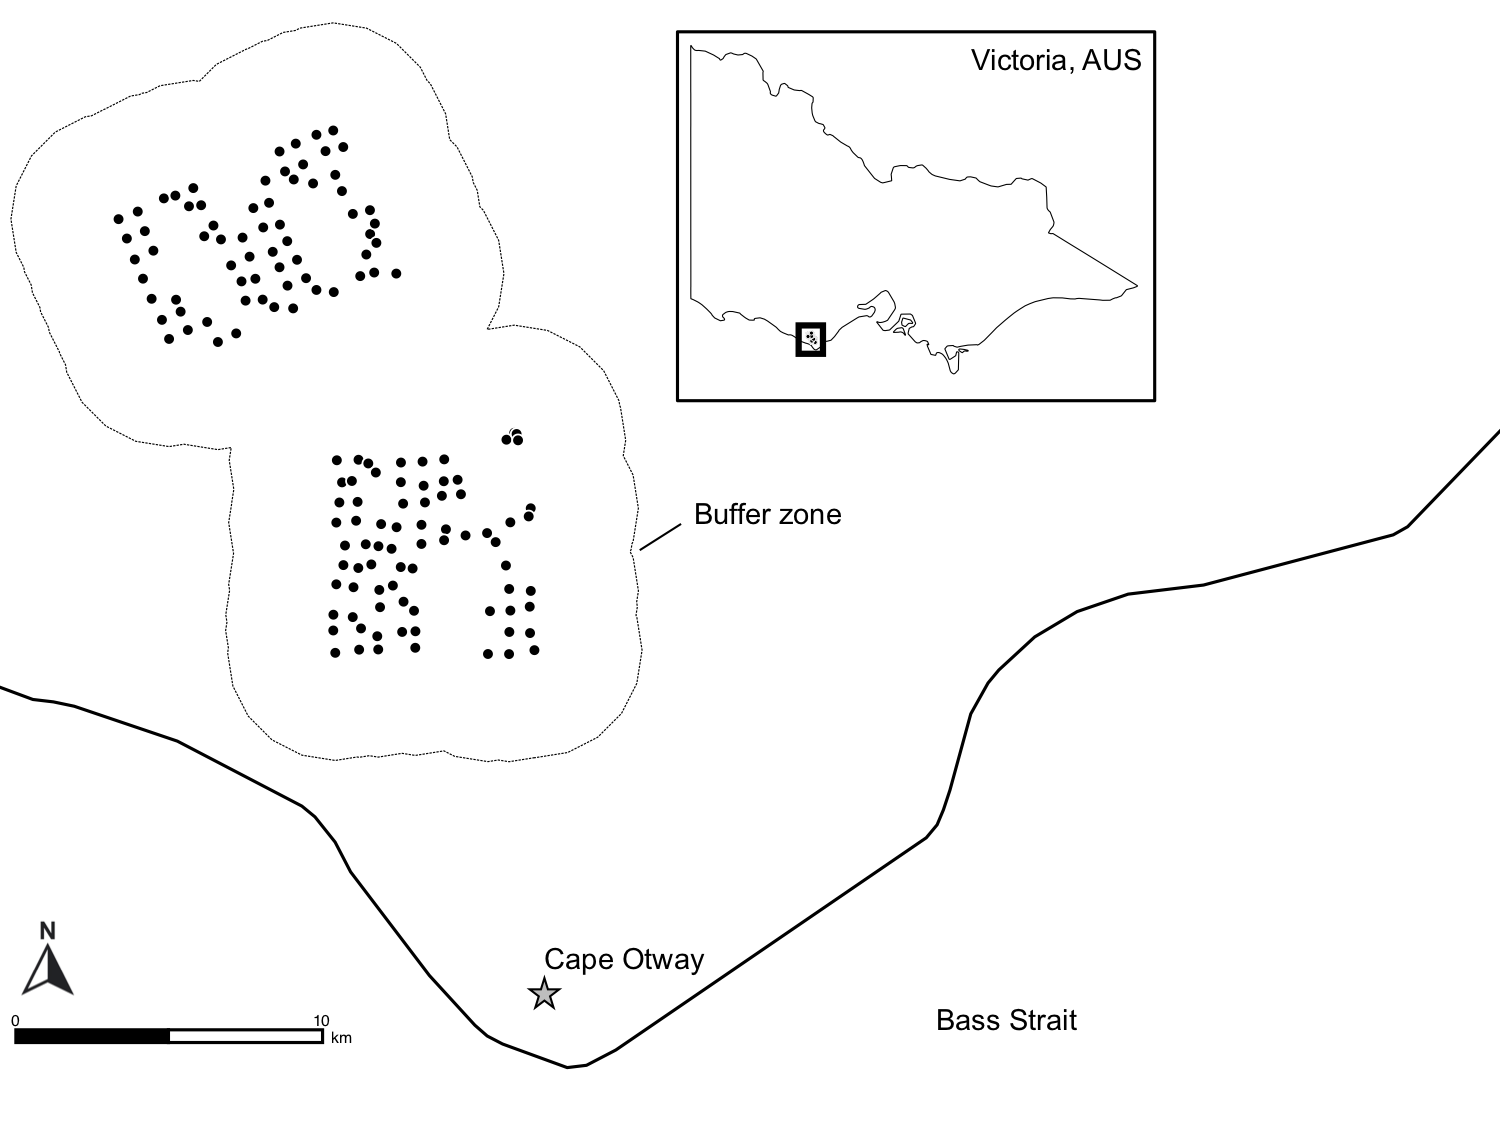
\includegraphics[width=1\linewidth]{figure/c2/c2_map} 

\caption{Study area, western Otway Ranges, Victoria, Australia, showing the location of the camera-trapping sites (black dots) within the 3500 m buffer zone (thin grey line).}\label{fig:otways17-map}
\end{figure}
\newpage

\hypertarget{results-2}{%
\section{Results}\label{results-2}}

We detected feral cats at 55\% of sites. Of these detections (1 detection = one or more visits of an individual/unidentifiable/unmarked cat to a camera-trap per 24-h occasion), 41\% were unmarked (black) cats. Of the marked cat detections, 89\% could be reliably identified to the individual-level -- 47 individuals were identified. The number of detections, number of identified individuals and mean distances moved were similar across the two camera-trapping grids (Table \ref{tab:otways17-stats}).

The top-ranked model estimated a density of 1.14 cats km\textsuperscript{-2} (95\% CI: 0.88 -- 1.47), with no difference in density between grids but a linear decrease in \emph{g}\textsubscript{0} over time (5.7\% decrease per week; Fig. \ref{fig:otways17-g0t}; Table \ref{tab:otways17-stats}). The second-ranked model (dAICc 1.74, Akaike weight 0.23) indicated that densities were slightly higher at the northern than southern grid, although confidence intervals overlapped substantially (Table \ref{tab:otways17-estimates}). The hazard-rate detector function best described the rate at which detection probability changed with the distance of the camera from the centre of a cat's home range (Table \ref{tab:otways17-detfn}). Estimates of feral cat density were robust to all model specifications, with the mean estimate varying by less than 0.2 cats km\textsuperscript{-2} between all models (Table \ref{tab:otways17-stats}).

\newpage

\(~\)

\(~\)

\(~\)
\begin{longtable}[]{@{}lccc@{}}
\caption{\label{tab:otways17-stats} Summary of raw camera survey data for feral cats in the Otway Ranges, Victoria, Australia, 2017.}\tabularnewline
\toprule
\begin{minipage}[b]{0.40\columnwidth}\raggedright
Summary statistic\strut
\end{minipage} & \begin{minipage}[b]{0.16\columnwidth}\centering
southern grid\strut
\end{minipage} & \begin{minipage}[b]{0.16\columnwidth}\centering
northern grid\strut
\end{minipage} & \begin{minipage}[b]{0.16\columnwidth}\centering
both grids\strut
\end{minipage}\tabularnewline
\midrule
\endfirsthead
\toprule
\begin{minipage}[b]{0.40\columnwidth}\raggedright
Summary statistic\strut
\end{minipage} & \begin{minipage}[b]{0.16\columnwidth}\centering
southern grid\strut
\end{minipage} & \begin{minipage}[b]{0.16\columnwidth}\centering
northern grid\strut
\end{minipage} & \begin{minipage}[b]{0.16\columnwidth}\centering
both grids\strut
\end{minipage}\tabularnewline
\midrule
\endhead
\begin{minipage}[t]{0.40\columnwidth}\raggedright
Number of camera sites\strut
\end{minipage} & \begin{minipage}[t]{0.16\columnwidth}\centering
73\strut
\end{minipage} & \begin{minipage}[t]{0.16\columnwidth}\centering
67\strut
\end{minipage} & \begin{minipage}[t]{0.16\columnwidth}\centering
140\strut
\end{minipage}\tabularnewline
\begin{minipage}[t]{0.40\columnwidth}\raggedright
Sites where cats detected (\%)\strut
\end{minipage} & \begin{minipage}[t]{0.16\columnwidth}\centering
51\strut
\end{minipage} & \begin{minipage}[t]{0.16\columnwidth}\centering
62\strut
\end{minipage} & \begin{minipage}[t]{0.16\columnwidth}\centering
55\strut
\end{minipage}\tabularnewline
\begin{minipage}[t]{0.40\columnwidth}\raggedright
Number of unmarked detection events\strut
\end{minipage} & \begin{minipage}[t]{0.16\columnwidth}\centering
47\strut
\end{minipage} & \begin{minipage}[t]{0.16\columnwidth}\centering
48\strut
\end{minipage} & \begin{minipage}[t]{0.16\columnwidth}\centering
95\strut
\end{minipage}\tabularnewline
\begin{minipage}[t]{0.40\columnwidth}\raggedright
Number of identifiable, marked detection events\strut
\end{minipage} & \begin{minipage}[t]{0.16\columnwidth}\centering
60\strut
\end{minipage} & \begin{minipage}[t]{0.16\columnwidth}\centering
59\strut
\end{minipage} & \begin{minipage}[t]{0.16\columnwidth}\centering
119\strut
\end{minipage}\tabularnewline
\begin{minipage}[t]{0.40\columnwidth}\raggedright
Number of unidentifiable, marked detection events\strut
\end{minipage} & \begin{minipage}[t]{0.16\columnwidth}\centering
10\strut
\end{minipage} & \begin{minipage}[t]{0.16\columnwidth}\centering
5\strut
\end{minipage} & \begin{minipage}[t]{0.16\columnwidth}\centering
15\strut
\end{minipage}\tabularnewline
\begin{minipage}[t]{0.40\columnwidth}\raggedright
Total number of identified individuals\strut
\end{minipage} & \begin{minipage}[t]{0.16\columnwidth}\centering
23\strut
\end{minipage} & \begin{minipage}[t]{0.16\columnwidth}\centering
24\strut
\end{minipage} & \begin{minipage}[t]{0.16\columnwidth}\centering
47\strut
\end{minipage}\tabularnewline
\begin{minipage}[t]{0.40\columnwidth}\raggedright
Number of cats resighted at different cameras\strut
\end{minipage} & \begin{minipage}[t]{0.16\columnwidth}\centering
8\strut
\end{minipage} & \begin{minipage}[t]{0.16\columnwidth}\centering
6\strut
\end{minipage} & \begin{minipage}[t]{0.16\columnwidth}\centering
14\strut
\end{minipage}\tabularnewline
\begin{minipage}[t]{0.40\columnwidth}\raggedright
Mean recapture distance (m)\strut
\end{minipage} & \begin{minipage}[t]{0.16\columnwidth}\centering
653\strut
\end{minipage} & \begin{minipage}[t]{0.16\columnwidth}\centering
774\strut
\end{minipage} & \begin{minipage}[t]{0.16\columnwidth}\centering
716\strut
\end{minipage}\tabularnewline
\begin{minipage}[t]{0.40\columnwidth}\raggedright
Maximum recapture distance (m)\strut
\end{minipage} & \begin{minipage}[t]{0.16\columnwidth}\centering
905\strut
\end{minipage} & \begin{minipage}[t]{0.16\columnwidth}\centering
1701\strut
\end{minipage} & \begin{minipage}[t]{0.16\columnwidth}\centering
1701\strut
\end{minipage}\tabularnewline
\bottomrule
\end{longtable}
\newpage

\(~\)

\(~\)

\(~\)
\begin{longtable}[t]{lllllllrrr}
\caption{\label{tab:otways17-estimates}Comparison of spatial mark-resight models and density estimates}\\
\toprule
\multicolumn{2}{c}{Model} & \multicolumn{4}{c}{Model comparison} & \multicolumn{4}{c}{Density estimate (cats km-2)} \\
\cmidrule(l{3pt}r{3pt}){1-2} \cmidrule(l{3pt}r{3pt}){3-6} \cmidrule(l{3pt}r{3pt}){7-10}
Density & g0 & K & AICc & dAICc & AICcwt & grid & estimate & lcl & ucl\\
\midrule
\endfirsthead
\caption[]{\label{tab:otways17-estimates}Comparison of spatial mark-resight models and density estimates \textit{(continued)}}\\
\toprule
\multicolumn{2}{c}{Model} & \multicolumn{4}{c}{Model comparison} & \multicolumn{4}{c}{Density estimate (cats km-2)} \\
\cmidrule(l{3pt}r{3pt}){1-2} \cmidrule(l{3pt}r{3pt}){3-6} \cmidrule(l{3pt}r{3pt}){7-10}
Density & g0 & K & AICc & dAICc & AICcwt & grid & estimate & lcl & ucl\\
\midrule
\endhead

\endfoot
\bottomrule
\endlastfoot
1 & T & 5 & 1568.84 & 0 & 0.71 & both & 1.14 & 0.88 & 1.47\\
grid & T & 6 & 1570.68 & 1.84 & 0.28 & north & 1.23 & 0.90 & 1.68\\
 &  &  &  &  &  & south & 1.05 & 0.78 & 1.42\\
1 & 1 & 4 & 1578.37 & 9.53 & 0.01 & both & 1.14 & 0.89 & 1.48\\
grid & 1 & 5 & 1579.66 & 10.82 & 0 & north & 1.25 & 0.91 & 1.72\\
\addlinespace
 &  &  &  &  &  & south & 1.04 & 0.77 & 1.40\\*
\end{longtable}
\emph{T = linear time trend}

\emph{K = number of parameters estimated}

\emph{AICc = Akaike's Information Criterion with small-sample adjustment}

\emph{dAICc = difference between AICc of this model and the model with smallest AICc}

\emph{AICcwt = AICc model weight}

\emph{lcl -- lower 95\% confidence limit}

\emph{ucl -- upper 95\% confidence limit}

\newpage

\hypertarget{discussion-2}{%
\section{Discussion}\label{discussion-2}}

Our work provides one of the first robust estimates of feral cat density for a temperate wet forest in Australia. Our estimate of 1.14 cats km\textsuperscript{-2} (95\% CI: 0.88 -- 1.47) is five times higher than that predicted by the Legge \emph{et al.} (2017) model for this location (0.17 - 0.23 cats km\textsuperscript{-2}), and more than three times higher than the predicted continental mean density for feral cats in `natural areas' (0.27 cats km\textsuperscript{-2}; 0.18 -- 0.45 cats km\textsuperscript{-2}; Legge \emph{et al.} 2017). The mesic coastal areas of Australia were previously thought to support the lowest densities of feral cats across the continent, particularly rugged and wet regions, such as rainforests (Dickman 1996; Johnson 2006; Legge \emph{et al.} 2017; McDonald \emph{et al.} 2017). Accordingly, feral cats were believed to have relatively less impact on native species in these environments (Burbidge \& Manly 2002; Doherty \emph{et al.} 2017; Woinarski \emph{et al.} 2017, 2018; Radford \emph{et al.} 2018; Murphy \emph{et al.} 2019). Our finding is therefore startling, and prompts a rethink about the threat that feral cats may pose to native fauna in mesic habitats.

The high density of feral cats in our study region likely reflects the high productivity of the landscape and abundant populations of some prey species. Our study region has the highest annual rainfall in Victoria (Bureau of Meteorology 2021), and live-trapping surveys in our study site show consistent, near saturation of small mammal traps, predominantly bush rats \emph{Rattus fuscipes} and \emph{Antechinus spp}. (Z. Banïkos, unpublished data). Several images from our study confirmed that feral cats prey upon these taxa. These small mammals may be relatively robust to introduced predators due to their high fecundity and generalist habitat requirements (e.g.~Banks 1999). However, by supporting high densities of feral cats, they may also facilitate high levels of predation on rarer and more vulnerable species (Smith \& Quin 1996), such as the now locally extinct smoky mouse \emph{Pseudomys fumeus} (Menkhorst \& Broome 2006). Significant declines and local extinctions of other small mammals have also been reported across the eastern Otways (Wayne \emph{et al.} 2017). Understanding temporal trends in these predator-prey dynamics and the relationships between introduced predators and their native primary and alternative prey is a key priority for future research.

The lack of apex predators and competitors in the Otway Ranges may also facilitate high feral cat densities. Dingoes \emph{Canis familiaris}--higher order predators (Johnson \emph{et al.} 2007)--and tiger quolls \emph{Dasyurus maculatus}--key competitors (Glen \& Dickman 2005)--are functionally extinct in the Otway Ranges. We detected foxes at 25\% of sites (M. Rees, unpublished data) but the extent to which foxes exert top-down control on feral cats is unclear. Changes in feral cat abundance, behaviour and/or diet have been observed in response to fox control (Molsher \emph{et al.} 2017; Hunter \emph{et al.} 2018), and the relationship could be further clarified using robust density estimates under experimental manipulations of fox density.

The belief that feral cat densities in Australia are lower in mesic forests than open habitats stems partly from the lack of robust density estimates from forests, and partly from observations that cats have greater hunting success and are more detectable in open microhabitats (McGregor \emph{et al.} 2014, 2015; Hohnen \emph{et al.} 2016; McDonald \emph{et al.} 2017) and select for savannah over rainforest (McGregor \emph{et al.} 2017). However, the variation in understorey structure (from extremely dense to relatively open) in our study region potentially creates ideal shelter and foraging habitat for feral cats, which often hunt along edges between dense and open vegetation (Doherty \emph{et al.} 2015). Our findings challenge the belief that cat density is low in mesic forests, and instead concur with the global pattern that feral cats have smaller, overlapping home ranges in productive, low-seasonal environments, resulting in higher population densities (Bengsen \emph{et al.} 2016).

Our surveys clearly need replicating in other mesic environments before they can be generalised. Nonetheless, higher than expected densities of feral cats in mesic and complex environments would have serious implications for biodiversity conservation. Feral cats are thought to be a key driver of the recent declines of critical-weight-range mammals in northern Australia (Woinarski \emph{et al.} 2010; Fisher \emph{et al.} 2014; Davies \emph{et al.} 2018). Contemporary mammal declines are also occurring in temperate Australia, including the Otway Ranges (Bilney \emph{et al.} 2010; Wayne \emph{et al.} 2017; Lindenmayer \emph{et al.} 2018). A better understanding of feral cat densities in these regions is essential for identifying key threatening processes and improving management outcomes.

In conclusion, our study shows that feral cats can occur at high densities in wet forests and cool temperate rainforests, contrary to previous expectations. Further research is needed to understand the impacts of this on native mammal populations, and the mechanisms that drive spatial variation in feral cat density, including the influence of habitat type, productivity, disturbance events and interactions with other predators. New spatial capture-recapture methods will likely play a powerful role in improving understanding of the ecology of this globally-significant predator. Our work provides a strong foundation for future investigations, as our methodology allows for robust evaluations of feral cat density, particularly under experimental manipulations and population comparisons.

\hypertarget{density}{%
\chapter{Quantifying mesopredator release: lethal control of an invasive apex predator alters feral cat density and detectability}\label{density}}

\hypertarget{abstract-3}{%
\section*{Abstract}\label{abstract-3}}
\addcontentsline{toc}{section}{Abstract}
\begin{enumerate}
\def\labelenumi{\arabic{enumi}.}
\item
  The mesopredator release hypothesis predicts that subordinate predator density will increase as apex predators decline. Persistent debate around mesopredator release in part reflects the lack of robust, replicated experiments to test this theory, and the use of population indices which confound changes in mesopredator density and detectability. This uncertainty has immediate impacts for conservationists who are faced with managing sympatric invasive predators.
\item
  We used replicating experimental designs and spatially explicit detection modelling to examine whether mesopredator release of the feral cat \emph{Felis catus} occurs in response to targeted control of the introduced red fox \emph{Vulpes vulpes}. We surveyed three Control-Impact paired landscapes in a region with long-term fox control (1080 poison-baiting), and conducted a Before-After-Control-Impact Paired Series experiment in another region. We identified 160 individual feral cats from 68,504 camera-trap nights to estimate feral cat density with spatial mark-resight models.
\item
  At a landscape scale (mean size: 169 km\textsuperscript{2}), lethal fox control was associated with a range of responses from a negligible to 3.7-fold increase in feral cat density. Consistent with the mesopredator release hypothesis, the degree of increase corresponded with variation in the duration and intensity of fox suppression. At a fine spatial scale (200 m), feral cat density had a consistent negative association with fox activity across both regions.
\item
  Feral cat detectability also varied across the (artificially manipulated) fox activity gradient. In one region, nonlinear models indicated that feral cats exhibited avoidance behaviours when foxes were rare, giving way to density suppression at high fox activity.
\item
  \emph{Synthesis and applications.} Our study provides replicated, experimental evidence that that apex predator suppression is associated with an increase in the density of a mesopredator. Mesopredator release can manifest as changes in both behaviour and density, distorting inference if these processes are not distinguished. Our results help explain why fox control does not consistently improve native prey persistence, suggesting integrated pest management may be necessary to improve conservation outcomes.
\end{enumerate}
\newpage

\hypertarget{introduction-3}{%
\section{Introduction}\label{introduction-3}}

Understanding species interactions is critical for effective invasive species management (Zavaleta \emph{et al.} 2001). When several invasive species co-occur, management actions that suppress the dominant invasive species may inadvertently benefit subordinate invasive species (Jackson 2015; Kuebbing \& Nuñez 2015). For example, the removal of a dominant invasive predator may increase the abundance of a subordinate invasive species directly by reducing top-down pressure, or indirectly by increasing the availability of shared resources; these are often referred to as mesopredator or competitor release, respectively (Crooks \& Soulé 1999; Ruscoe \emph{et al.} 2011; Doherty \& Ritchie 2017). The release of subordinate invasive species, particularly predators, can have serious negative implications for native taxa and ecosystem function (Courchamp \emph{et al.} 1999; Ballari \emph{et al.} 2016). However, integrated invasive predator management is often far more costly and less feasible than single species control, and so it is important to identify when the extra cost is justified (Bode \emph{et al.} 2015).

Most knowledge of mesopredator release stems from unreplicated `natural experiments' (e.g.~range contractions - Crooks \& Soulé 1999) or ad-hoc management interventions (e.g.~invasive species eradications - Rayner \emph{et al.} 2007). Does mesopredator release still occur when apex predators are suppressed but not completely removed? The occurrence, nature (positive or negative, direct or indirect) and strength of predator interactions can vary among species assemblages, predation risk, environmental productivity, management regimes and other landscape contexts (Hastings 2001; Finke \& Denno 2004; Elmhagen \& Rushton 2007; Newsome \emph{et al.} 2017; Alston \emph{et al.} 2019). Replicating management programs in an experimental framework is logistically challenging, but important for understanding these complexities, discriminating between plausible hypotheses and producing generalisable results to inform effective pest management (Glen \& Dickman 2005; Hayward \emph{et al.} 2015; Christie \emph{et al.} 2019; Smith \emph{et al.} 2020).

Another source of uncertainty around the mesopredator release hypothesis stems from the inability of traditional survey and modelling approaches to distinguish behavioural from numerical population processes (Hayward \emph{et al.} 2015; Stephens \emph{et al.} 2015). Suppression of an apex predator may simultaneously change the behaviour and the density of a mesopredator, both of which influence detection rates (Broadley \emph{et al.} 2019; Rogan \emph{et al.} 2019). This makes it difficult to interpret observed changes in naive indices of mesopredator activity or occupancy in relation to changes in apex predator populations, even if the study has an experimental design. Unbiased estimates of invasive predator density are also important for setting meaningful control targets and inferring impacts on native prey (Moseby \emph{et al.} 2019). Spatial capture-recapture methods offer a solution by separating behavioural and observational processes from population density, which is estimated within a defined spatial resolution (Borchers \& Efford 2008).

Predation by two invasive species, the red fox \emph{Vulpes vulpes} (hereafter `fox') and feral cat \emph{Felis catus} (hereafter `cat'), has played a major role in Australia's high rates of mammalian extinction (Woinarski \emph{et al.} 2015). Integrated pest management programs are rare; instead, foxes are far more commonly controlled than cats, as they are more susceptible to poison-baiting, have greater direct economic impacts and fewer legal impediments to control (Reddiex \emph{et al.} 2007; McLeod \& Saunders 2014). Nonetheless, cats are one of the most widespread and damaging vertebrate predator species (Medina \emph{et al.} 2011; Doherty \& Ritchie 2017; Legge \emph{et al.} 2020). As foxes are larger-bodied (\textasciitilde2 kg difference) and have high dietary overlap with cats (Stobo-Wilson \emph{et al.} 2021a, b), the mesopredator release hypothesis (Soulé \emph{et al.} 1988) predicts that the impacts of cats on shared prey species will increase as fox populations are suppressed. This is alarming because feral cats are extremely difficult to manage in open populations (Fisher \emph{et al.} 2015; Lazenby \emph{et al.} 2015).

Evidence that foxes suppress cats is inconclusive (Hunter \emph{et al.} 2018). In parts of Australia where the native apex mammalian predator (the dingo \emph{Canis familiaris}) is functionally extinct and introduced foxes are the largest terrestrial mammalian predator, four studies have observed an increase in cat detections following fox control (Risbey \emph{et al.} 2000; Marlow \emph{et al.} 2015; Stobo-Wilson \emph{et al.} 2020). However, two other studies in similar systems did not see any change (Towerton \emph{et al.} 2011; Molsher \emph{et al.} 2017). A further study with spatial replication detected an increase at one site but not another (Davey \emph{et al.} 2006), and another observed a decrease in cat activity (Claridge \emph{et al.} 2010). No prior studies have directly estimated cat density in response to fox control.

We experimentally investigated the role of introduced foxes in top-down suppression of cat density in two regions of south-eastern Australia. Our experiments had a replicated Control-Impact design in the region with long-term fox control, and a Before-After Control-Impact Paired Series (BACIPS) design in the region with newly implemented fox control. Foxes and cats are the only functional terrestrial mammalian predators in these regions, and each region included at least one area in which foxes were subject to continuous lethal poison-baiting (hereafter `impact landscape'), and a paired area where foxes were not controlled (hereafter `non-impact landscape'). This allowed a sharp focus on the interactions between the two invasive predators, across a gradient of apex predator (fox) occurrence. In accordance with the mesopredator release hypothesis, we predicted that: (1) cat density would be negatively correlated with fox occurrence at a fine spatial scale, and (2) fox control would increase cat density at a landscape scale. We based inference on direct estimates of cat density using spatially explicit mark-resight models.

\newpage

\hypertarget{methods-3}{%
\section{Methods}\label{methods-3}}

\hypertarget{study-area-3}{%
\subsection{Study area}\label{study-area-3}}

We conducted our study across two regions of south-west Victoria, Australia (Fig. \ref{fig:density-map}). The native temperate forests in both regions are fragmented to varying degrees, primarily by livestock farming and tree plantations. Although once widespread, native dingoes are now absent throughout, and a native mesopredator, the tiger quoll \emph{Dasyurus maculatus} is long absent from the Glenelg region and extremely rare in the Otway Ranges (last sighted in 2014 despite extensive camera-trapping). The terrestrial mammalian predator guild is therefore depauperate, with foxes and cats being the primary functional mammalian terrestrial predators; birds of prey and snakes are the only other medium-large carnivores present.

Our study landscapes in the Glenelg region, Gunditjmara country, were primarily lowland forest and heathy woodland. The area receives an average annual rainfall of 700 mm (Bureau of Meteorology 2021) and has gently undulating terrain. The region frequently experiences prescribed burns and wildfires, creating a mosaic of fire histories and vegetation complexity. Our study landscapes in the Otway region were in the western section of the Otway Ranges on Gadubanud country. Rainfall here is more than twice as high as the Glenelg region. The vegetation is a mosaic of shrubby wet forest and cool temperate rainforest, with the northern landscape bordering on a large heathy woodland. This region rarely experiences fire and is nearly ten times more rugged than the Glenelg region (based on the terrain ruggedness index; Riley \emph{et al.} 1999).

Government land managers conduct ongoing targeted fox control for biodiversity conservation across broad sections of each region. In these sections, manufactured poison baits (FoxOff, Animal Control Technologies, Somerton) containing 3 mg of sodium mono-fluroacetate (1080) are buried at a depth of 12-15 cm at 1-km intervals along accessible forest tracks and roads (Fig. \ref{fig:density-map}). Different road densities across the two regions result in variable poison-bait densities. Other large sections within each region are maintained without fox control.

\hypertarget{study-design-and-camera-trapping}{%
\subsection{Study design and camera-trapping}\label{study-design-and-camera-trapping}}

We designed experiments around the implementation of fox-baiting in each region. We simultaneously surveyed one impact and one non-impact landscape within a region at a time. Each pair of impact and non-impact landscapes was chosen based on similarity in vegetation groups, with the aim of maintaining spatial independence with respect to predator daily movements.

In the Glenelg region, we used a replicated control-impact design to compare three impact landscapes that have been poison-baited for foxes at fortnightly intervals for more than 13 years with three paired non-impact landscapes. We surveyed Cobboboonee National Park (impact) and Annya State Forest (non-impact) in January -- April 2018 (`replicate 1'), Mt Clay State Forest/Narrawong Flora Reserve (hereafter `Mt Clay'; impact) and Hotspur State Forest (non-impact) in April -- June 2018 (`replicate 2'), and Lower Glenelg National Park (LGNP) South (impact) and LGNP North (non-impact) in March -- May 2021 (`replicate 3'). For replicates 1 and 2, the paired landscapes were separated by at least 8 km, a distance very unlikely to be traversed regularly by these invasive predators (Hradsky \emph{et al.} 2017). LGNP South and North are separated by the Glenelg river, which is impassable by terrestrial animals.

In the Otway region, we used a before-after control-impact paired series (BACIPS) design to assess changes related to the introduction of a fox control program. We deployed camera-trap grids in a pair of impact -- non-impact landscapes from June to September in three years (2017, 2018, 2019), in the Great Otway National Park and Otway Forest Park. Our first survey occurred approximately three months before fox-baiting began. Fox-baiting commenced in the impact landscape in November 2017. Poison baits were replaced weekly for six weeks until December 2017, before changing to monthly bait replacement until July 2018. The second survey was conducted six months after fox-baiting commenced, however poison bait replacement lapsed from near the beginning of the survey until nearly three months afterwards. Fox-baiting at monthly intervals recommenced in December 2018, six months prior to the start of the final survey (Fig. \ref{fig:density-camop}). The impact and non-impact landscapes were at least 4.2 km apart through dense forest, a distance unlikely to be regularly traversed by these invasive predators, although possible (Hradsky \emph{et al.} 2017). In this study, and a concurrent study which identified individual foxes through genetic sampling (M. Le Pla et al., in review), we found no evidence that either foxes or cats moved between the impact and non-impact landscapes.

In each landscape, we established a grid of 49 -- 110 sites (mean = 88), averaging 448 m apart (range: 194 -- 770 m). At each site, we set up a Reconyx trail camera (Reconyx, Holmen, Wisconsin) with an infrared flash and temperature-in-motion detector on a tree, facing a tuna oil lure; see Appendix C section \ref{density-app-field} for details. Overall, we deployed 1051 functional camera-traps, which operated for an average of 65 days (range: 12 -- 93 days), totalling 68,504 trap nights (Table \ref{tab:density-stats}).

\hypertarget{individual-feral-cat-identification}{%
\subsection{Individual feral cat identification}\label{individual-feral-cat-identification}}

We sorted the camera-trap images of cats into five categories based on coat type: black, mackerel tabby, classic tabby, ginger and other; Fig. \ref{fig:density-cat-photo}, and identified individual feral cats within each category; see Appendix C section \ref{density-app-id} for details. In the Otway region, 40\% of cat detections were of black cats with few identifiable markings, so we did not attempt to identify any black cats here. In the Glenelg region, black cats were rarer (not detected at two landscapes) and often more distinctive, and so we could identify some individuals (Table \ref{tab:density-stats}).

\hypertarget{density-methods-fox}{%
\subsection{Spatial fox occurrence}\label{density-methods-fox}}

We could not use raw fox presence-absence data from the camera-traps to predict cat density, as spatial mark-resight models require covariate values for each grid cell in which density is estimated (see Section \ref{density-methods-smr}). Instead, we generated a spatially-interpolated layer of the probability of fox occurrence for each study landscape, using fox presence-absence data for each camera-trap site and binomial generalised additive mixed-effects models (Wood 2017). These models allow efficient nonlinear spatial estimates, but do not account for imperfect detection.

We built the fox occurrence models using the `mgcv' R-package (version 1.3.1; Wood 2011). We modelled fox presences and absences (response variable) across space (explanatory variable) separately for each region, with a duchon spline spatial smooth; these provide better predictions at the edge of surveyed space than other splines (Miller \& Wood 2014). In the Otway region, we included a random intercept for each camera-trap site to account for repeat sampling and did not share spatial information across years. Differences in camera-trap deployment lengths were accounted for using a model offset.

\hypertarget{density-methods-smr}{%
\subsection{Spatial mark-resight models of feral cat density}\label{density-methods-smr}}

We used a spatial capture-recapture approach to estimate cat density (Borchers \& Efford 2008). These models use counts of detections and non-detections of individual animals at trap locations (accounting for trap-specific survey effort) to estimate the location of each individual's activity centre. They commonly assume that individuals have approximately circular home ranges, spend the majority of time in the centre of their range (`activity centre'), and that the probability of observing an individual decreases with distance from the activity centre. Two detectability parameters govern this process: \emph{g}\textsubscript{0}, the probability of detecting an individual per occasion in their activity centre, and sigma: a spatial scale parameter which relates to home range size. Multiple candidate shapes for the decline in detectability with distance from the activity centre (`detection function') can be modelled. Spatial capture-recapture models have been extended to consider situations where not all individuals in a population are identifiable (i.e., some are unmarked; Chandler \& Royle 2013). These models typically assume unmarked individuals to be a random sample of the population, sharing the same detection process as marked individuals, allowing density to be estimated for the entire population.

We used closed population, sighting-only, spatial mark-resight models to estimate cat density using the maximum likelihood `secr' R-package (Efford 2021). Detections of the `mark status uncertain' category (unidentifiable cats), cannot be handled in the `secr' R package; we added them to as `unmarked' detections (black cats) rather than discard them (following Moseby \emph{et al.} 2020). We condensed unmarked detection histories to a binary presence-absence record per each camera-trap for a 24-hour length duration (`occasion'), beginning at midday. We ran separate models for each region and treated each camera-trap grid deployment as a `session'. We created a 4000-m buffer zone around each site (which was truncated by the river in LGNP), and estimated cat density at a 200-m grid cell resolution within this area. These habitat mask specifications were based on initial model trials and our knowledge of cat behaviour in these regions; the aim was to ensure density was estimated over a large enough area to encompass the activity centres of all cats exposed to our camera-traps, at a fine enough spatial scale to minimise bias in density estimates.

For each region, we ran four sets of models. We chose (1) between half-normal and exponential detection functions and (2) `base model' covariates to carry through to subsequent model sets, (3) tested for associations between fox occurrence and cat density at a fine spatial scale, and (4) experimentally evaluated the effect of fox control on cat density at the landscape scale. Each step is described in more detail below. We compared competing models using small-sample corrected Akaike Information Criterion (hereafter `AIC\textsubscript{c}') scores (Burnham \& Anderson 2004) and examined the confidence intervals around estimated model coefficients. Each step is described in more detail below.

The second set of models established the base covariates for each region. We hypothesised that cat detectability might decrease over each survey due to the scent of the tuna oil lure fading. To account for this, we modelled a linear trend in \emph{g}\textsubscript{0} over the survey duration for each camera-trap. We further hypothesised that cat density might differ between vegetation types. We classed the vegetation into three dominant types for each region: cleared land, heathy vegetation, and either dry forest (Glenelg region) or wet forest (Otway region); see see Appendix C section \ref{density-app-veg} for details. We compared these covariates as single and additive models, as well as to a `null model' (density and detectability constant) - carrying supported covariates forward to subsequent model fits.

The third set of models directly tested the associations between fox occurrence and cats within each region. We tested three hypotheses for each region: (i) fox occurrence only affects cat density, (ii) fox occurrence only affects cat detectability (both \emph{g}\textsubscript{0} and sigma concurrently; Efford \& Mowat 2014), (iii) fox occurrence affects the density and the detectability of cats, against (iv) the null hypothesis that there was no association between fox occurrence and cats. We used the spatial fox occurrence estimates (detailed in Section \ref{density-methods-fox}) as the explanatory variable. As predator associations may be nonlinear (Johnson \& VanDerWal 2009), we tested these effects as linear and non-linear terms using regression splines (generalised additive models called within the `secr' R-package). We included year as a cat density covariate in all the Otway region models to account for repeat sampling and compared to a null model without any fox occurrence effects using AIC\textsubscript{c} scores.

The fourth set of models examined the effects of fox-baiting at a landscape scale within each region. We fitted a model that estimated cat density separately for each landscape, and used AIC\textsubscript{c} scores to choose whether to model detectability as a function of predicted fox occurrence (as per hypothesis ii in the second set of models above) or constant. We then derived the response ratio (estimated difference in cat density in the impact landscape relative to the paired non-impact landscape, back-transformed to the response scale) for the top-ranked model. We used visual inspection of the 95\% confidence intervals around the density estimates to evaluate whether fox control increased cat density at a landscape level (Cumming \& Finch 2005). For the Glenelg region (replicated control-impact design), we assessed whether each confidence interval around the relative difference in cat density in the impact landscape to the paired non-impact landscape (i.e., `response-ratio') overlapped one; overlap would indicate no difference in cat density. For the Otway region (BACIPS design), we assessed how much the confidence intervals around the estimated difference between impact and non-impact landscapes overlapped between years; we expected that the response-ratio would increase over the years, indicating an increase in cat density following the introduction of fox control.

\newpage

\(~\)

\(~\)

\(~\)
\begin{figure}

{\centering 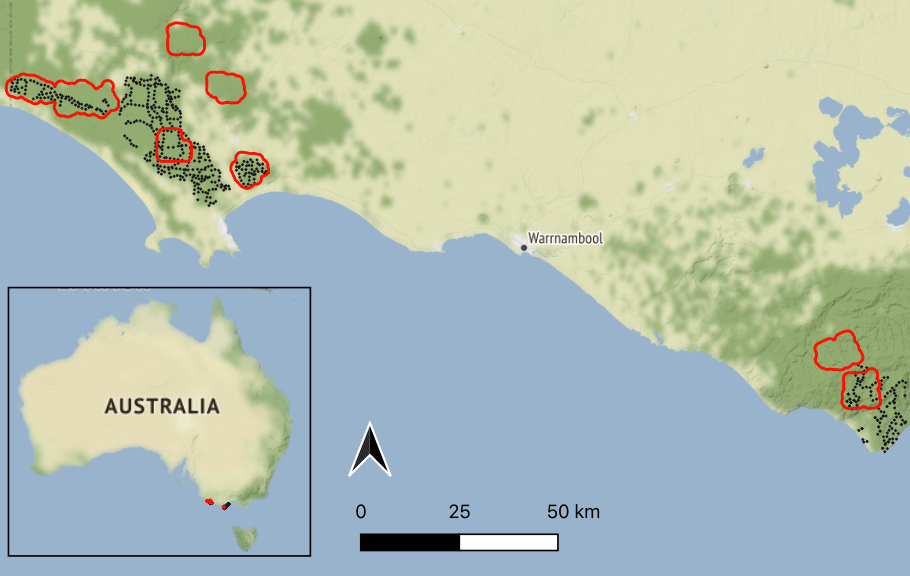
\includegraphics[width=1\linewidth]{figure/c3/fig1} 

}

\caption{Locations of our eight study landscapes in south-west Victoria, Australia (red outlines). Note the two Lower Glenelg National Park landscapes in the far west are shown as one but are separated by a river. Locations of fox poison-bait stations are denoted by black dots. The Glenelg region is to the west and Otway region to the east. Native vegetation is indicated by dark green, with hill shading. \textit{Map tiles by Stamen Design, under CC BY 3.0, map data by OpenStreetMap, under CC BY SA.}}\label{fig:density-map}
\end{figure}
\newpage

\hypertarget{results-3}{%
\section{Results}\label{results-3}}

\hypertarget{fox-occurrence}{%
\subsection{Fox occurrence}\label{fox-occurrence}}

In the Glenelg region, there was a clear difference in fox occurrence between paired impact (poison-baited) and non-impact landscapes for replicates 1 and 3, but only a marginal difference for replicate 2 (Fig. \ref{fig:foxplot}). In the Otway region, fox occurrence increased by 22\% in the non-impact landscape, and decreased by 43\% in the impact landscape over the three years (occurrence probability averaged at each camera-trap in the landscape). Fox occurrence in the Otway region was generally lower than the Glenelg region, with less fine-scale spatial variation. For example, fox occurrence was predicted to be spatially consistent across the entire Otway region in 2018 (Fig. \ref{fig:foxplot}). Fox model summaries and spatial standard error estimates are presented in Appendix C section \ref{density-app-fox}.

\hypertarget{feral-cats-in-the-glenelg-region}{%
\subsection{Feral cats in the Glenelg region}\label{feral-cats-in-the-glenelg-region}}

Across the six landscapes in the Glenelg region, we recorded 251 cat detections from 32,232 camera-trap nights (Table \ref{tab:density-stats}). We were able to identify 64\% of cat detections to the individual level; a total of 67 cats (6 -- 13 individuals per landscape). The exponential detector function was supported over the half-normal function (Table \ref{tab:density-aic-g-1}). The null model was more strongly supported than models with vegetation impacts on cat density and/or linear time trends on \emph{g}\textsubscript{0} (Table \ref{tab:density-aic-g-2}).

At a fine spatial scale, the model with a linear relationship between fox occurrence and cat density was strongly supported (AIC\textsubscript{c} 2.76 better than the null; Table \ref{tab:density-aic-g-3}). It indicated that cat density declined as fox occurrence increased (-0.32; 95\% CI: -0.57 - -0.07; Fig. \ref{fig:dcor}). There was no evidence of an impact of fox occurrence on cat detectability (Table \ref{tab:density-aic-g-3}). Regression splines added additional model parameters without changing predictions (Fig. \ref{fig:dcor}), and so, all nonlinear models ranked below their linear counterparts (Table \ref{tab:density-aic-g-3}).

Our hypothesis that cat density would be higher in landscapes with fox control was supported for the first and third replicate pairs: estimated cat densities were 2.5 (95\% CI: 1.5 - 4.2) and 3.7 (95\% CI: 1.4 - 9.5) times higher in the impact landscape than the paired non-impact landscape, respectively (Fig. \ref{fig:diffg}). For the second landscape pair, however, the estimated difference was positive but negligible (1.1; 95\% CI: 0.69 - 1.69). At the landscape level, there was some evidence that cat detectability was affected by fox occurrence; however the AIC\textsubscript{c} score was only 0.95 units better than the constant detectability model (Table \ref{tab:density-aic-g-4}) and the estimated effects were weak with high uncertainty. The detectability of cats in their activity centre (\emph{g}\textsubscript{0}) tended to increase with the probability of fox occurrence (0.24; 95\% CI: -0.32 - 0.80), as did sigma (0.13; 95\% CI: -0.14 - 0.41).

\hypertarget{feral-cats-in-the-otway-region}{%
\subsection{Feral cats in the Otway region}\label{feral-cats-in-the-otway-region}}

In the Otway region, we recorded 970 cat detections from 36,272 camera-trap nights (Table \ref{tab:density-stats}). We were able to identify 53\% of cat detections to the individual level; a total of 93 cats (20 -- 30 individuals per landscape). The exponential detector function was strongly supported over the half-normal function (Table \ref{tab:density-aic-o-1}). The null model was more strongly supported than the models with vegetation impacts on cat density and/or linear time trends on \emph{g}\textsubscript{0} (Table \ref{tab:density-aic-o-2}).

There was some evidence that cat density was negatively correlated with fox occurrence at a fine spatial scale: the two top-ranked models included a linear and a non-linear effect of fox occurrence on cat density, respectively; however, a model without a fox occurrence term received similar support (dAIC\textsubscript{c} = 0.80; Table \ref{tab:density-aic-o-3}). The 95\% confidence interval around the linear coefficient from the top-ranked model marginally overlapped zero (-0.26; 95\% CI: -0.55 - 0.02) indicating that cat density declined as fox occurrence increased in the Otways at a similar rate to Glenelg, but with slightly greater uncertainty (Fig. \ref{fig:dcor}). However, the equivalent nonlinear model predicted that cat density only declined (at a steeper rate) in the mid-high range of fox occurrence probability (Fig. \ref{fig:dcor}). Equivalent pairs of linear model and nonlinear models were indistinguishable based on AIC\textsubscript{c} scores (Table \ref{tab:density-aic-o-3}).
There was also strong support for an effect of fox occurrence on cat detectability at a fine spatial scale (Fig. \ref{fig:detcor}; Table \ref{tab:density-aic-o-4}). Where fox occurrence was higher, cats were less detectable in their activity centres (i.e., negative association with \emph{g}\textsubscript{0}; -0.69; 95\% CI: -1.11 - -0.27; Fig. \ref{fig:detcor}A) and ranged further (i.e., positive association with sigma; coefficient 0.30; 95\% CI: 0.13 - 0.47; Fig. \ref{fig:detcor}B). The equivalent nonlinear model predicted detectability changes to have occurred only in the low-mid range of fox occurrence (Fig. \ref{fig:detcor}).

Our hypothesis that cat density in the impact landscape would increase relative to the non-impact landscape with fox control was supported, however there was considerable uncertainty. Cat density tended to be lower in the impact than non-impact landscape prior to fox-baiting (i.e., in 2017), although the confidence intervals for the two density estimates overlapped substantially (Fig. \ref{fig:diffo}). In 2018, cat density decreased in the non-impact landscape and increased in the impact landscape, converging to near-identical density estimates. These patterns continued into 2019, with cat density now somewhat higher in the impact landscape than non-impact landscape. Overlap in the response ratio confidence intervals for successive years was high, but the comparison between 2017 to 2019 suggests a meaningful increase in cat density at the impact landscape relative to the non-impact landscape (Fig. \ref{fig:diffo}B). Like the fine scale model, there was strong evidence that cat detectability was impacted by fox occurrence (Table \ref{tab:density-aic-o-4}).

\newpage

\(~\)

\(~\)

\(~\)
\begin{figure}

{\centering 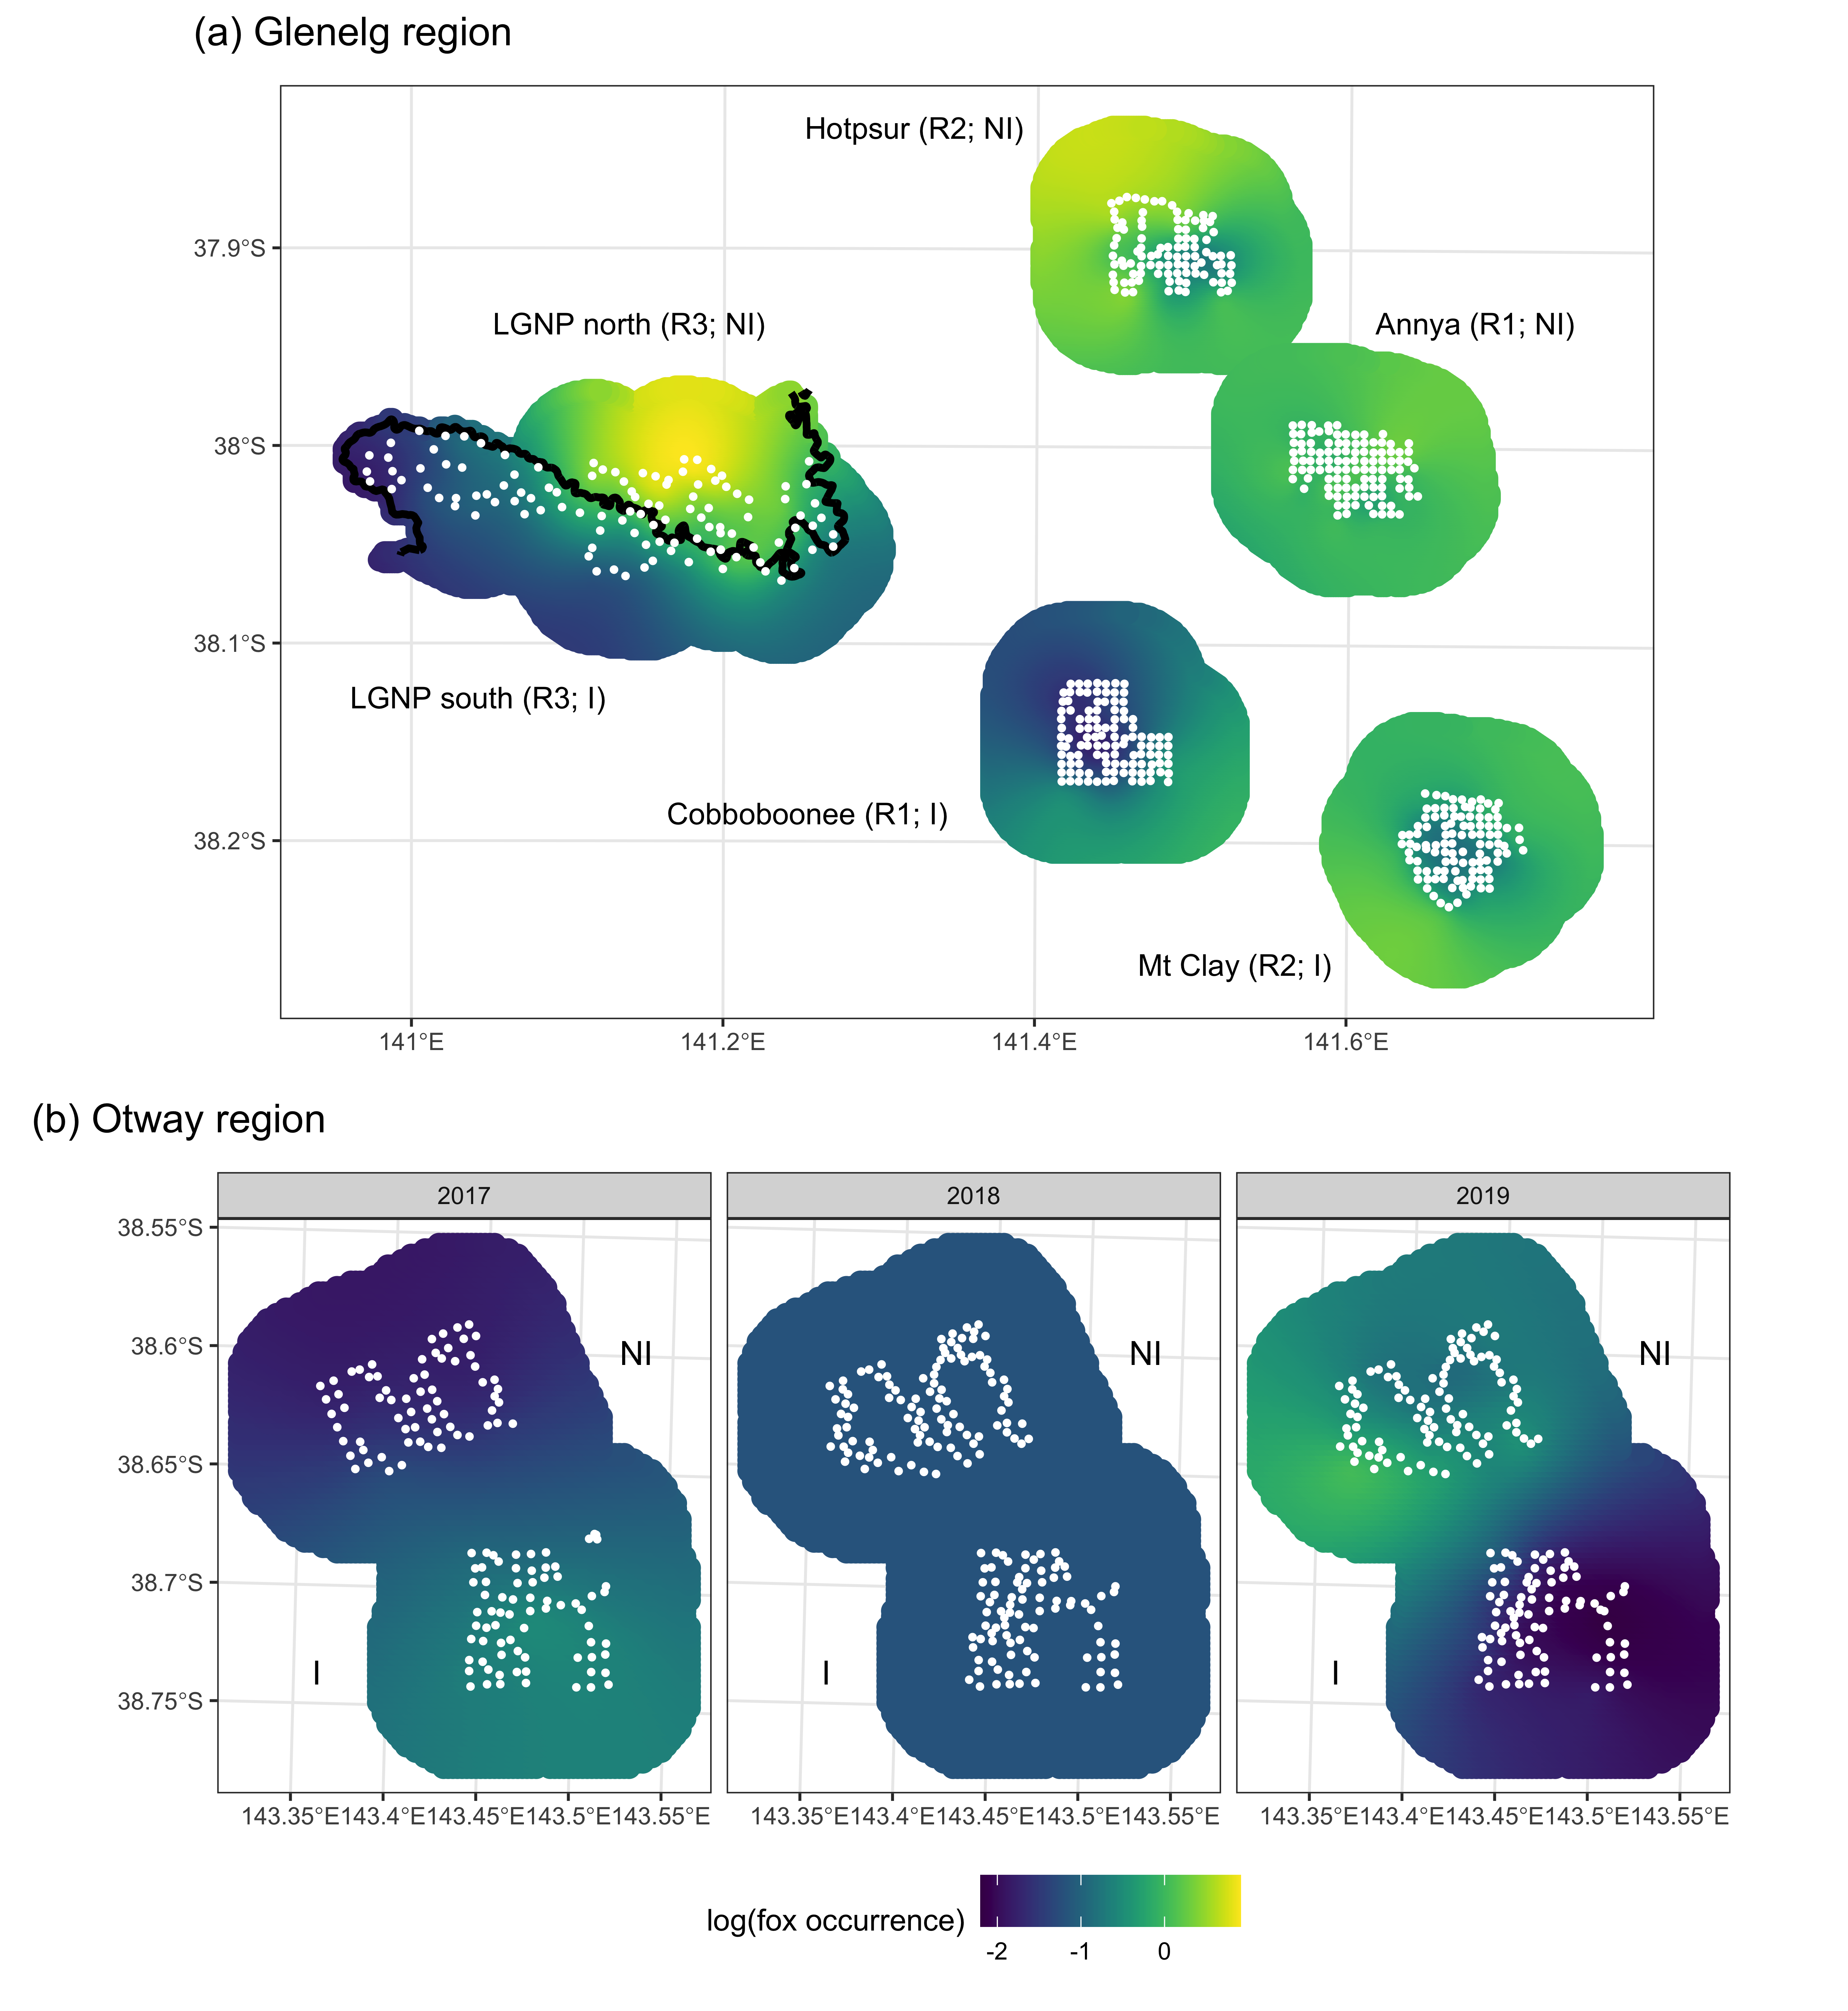
\includegraphics[width=1\linewidth]{figure/c3/fig2_600dpi} 

}

\caption{Predicted red fox \textit{Vulpes vulpes} occurrence derived from generalised additive models within each impact (I) and paired non-impact (NI) landscape in the Glenelg (a) and Otway (b) regions, Australia. White dots represent camera-trap sites. Predicted fox occurrence was used as a predictor of feral cat Felis catus density in the spatial mark-resight models.}\label{fig:foxplot}
\end{figure}
\newpage

\(~\)

\(~\)

\(~\)
\begin{figure}

{\centering 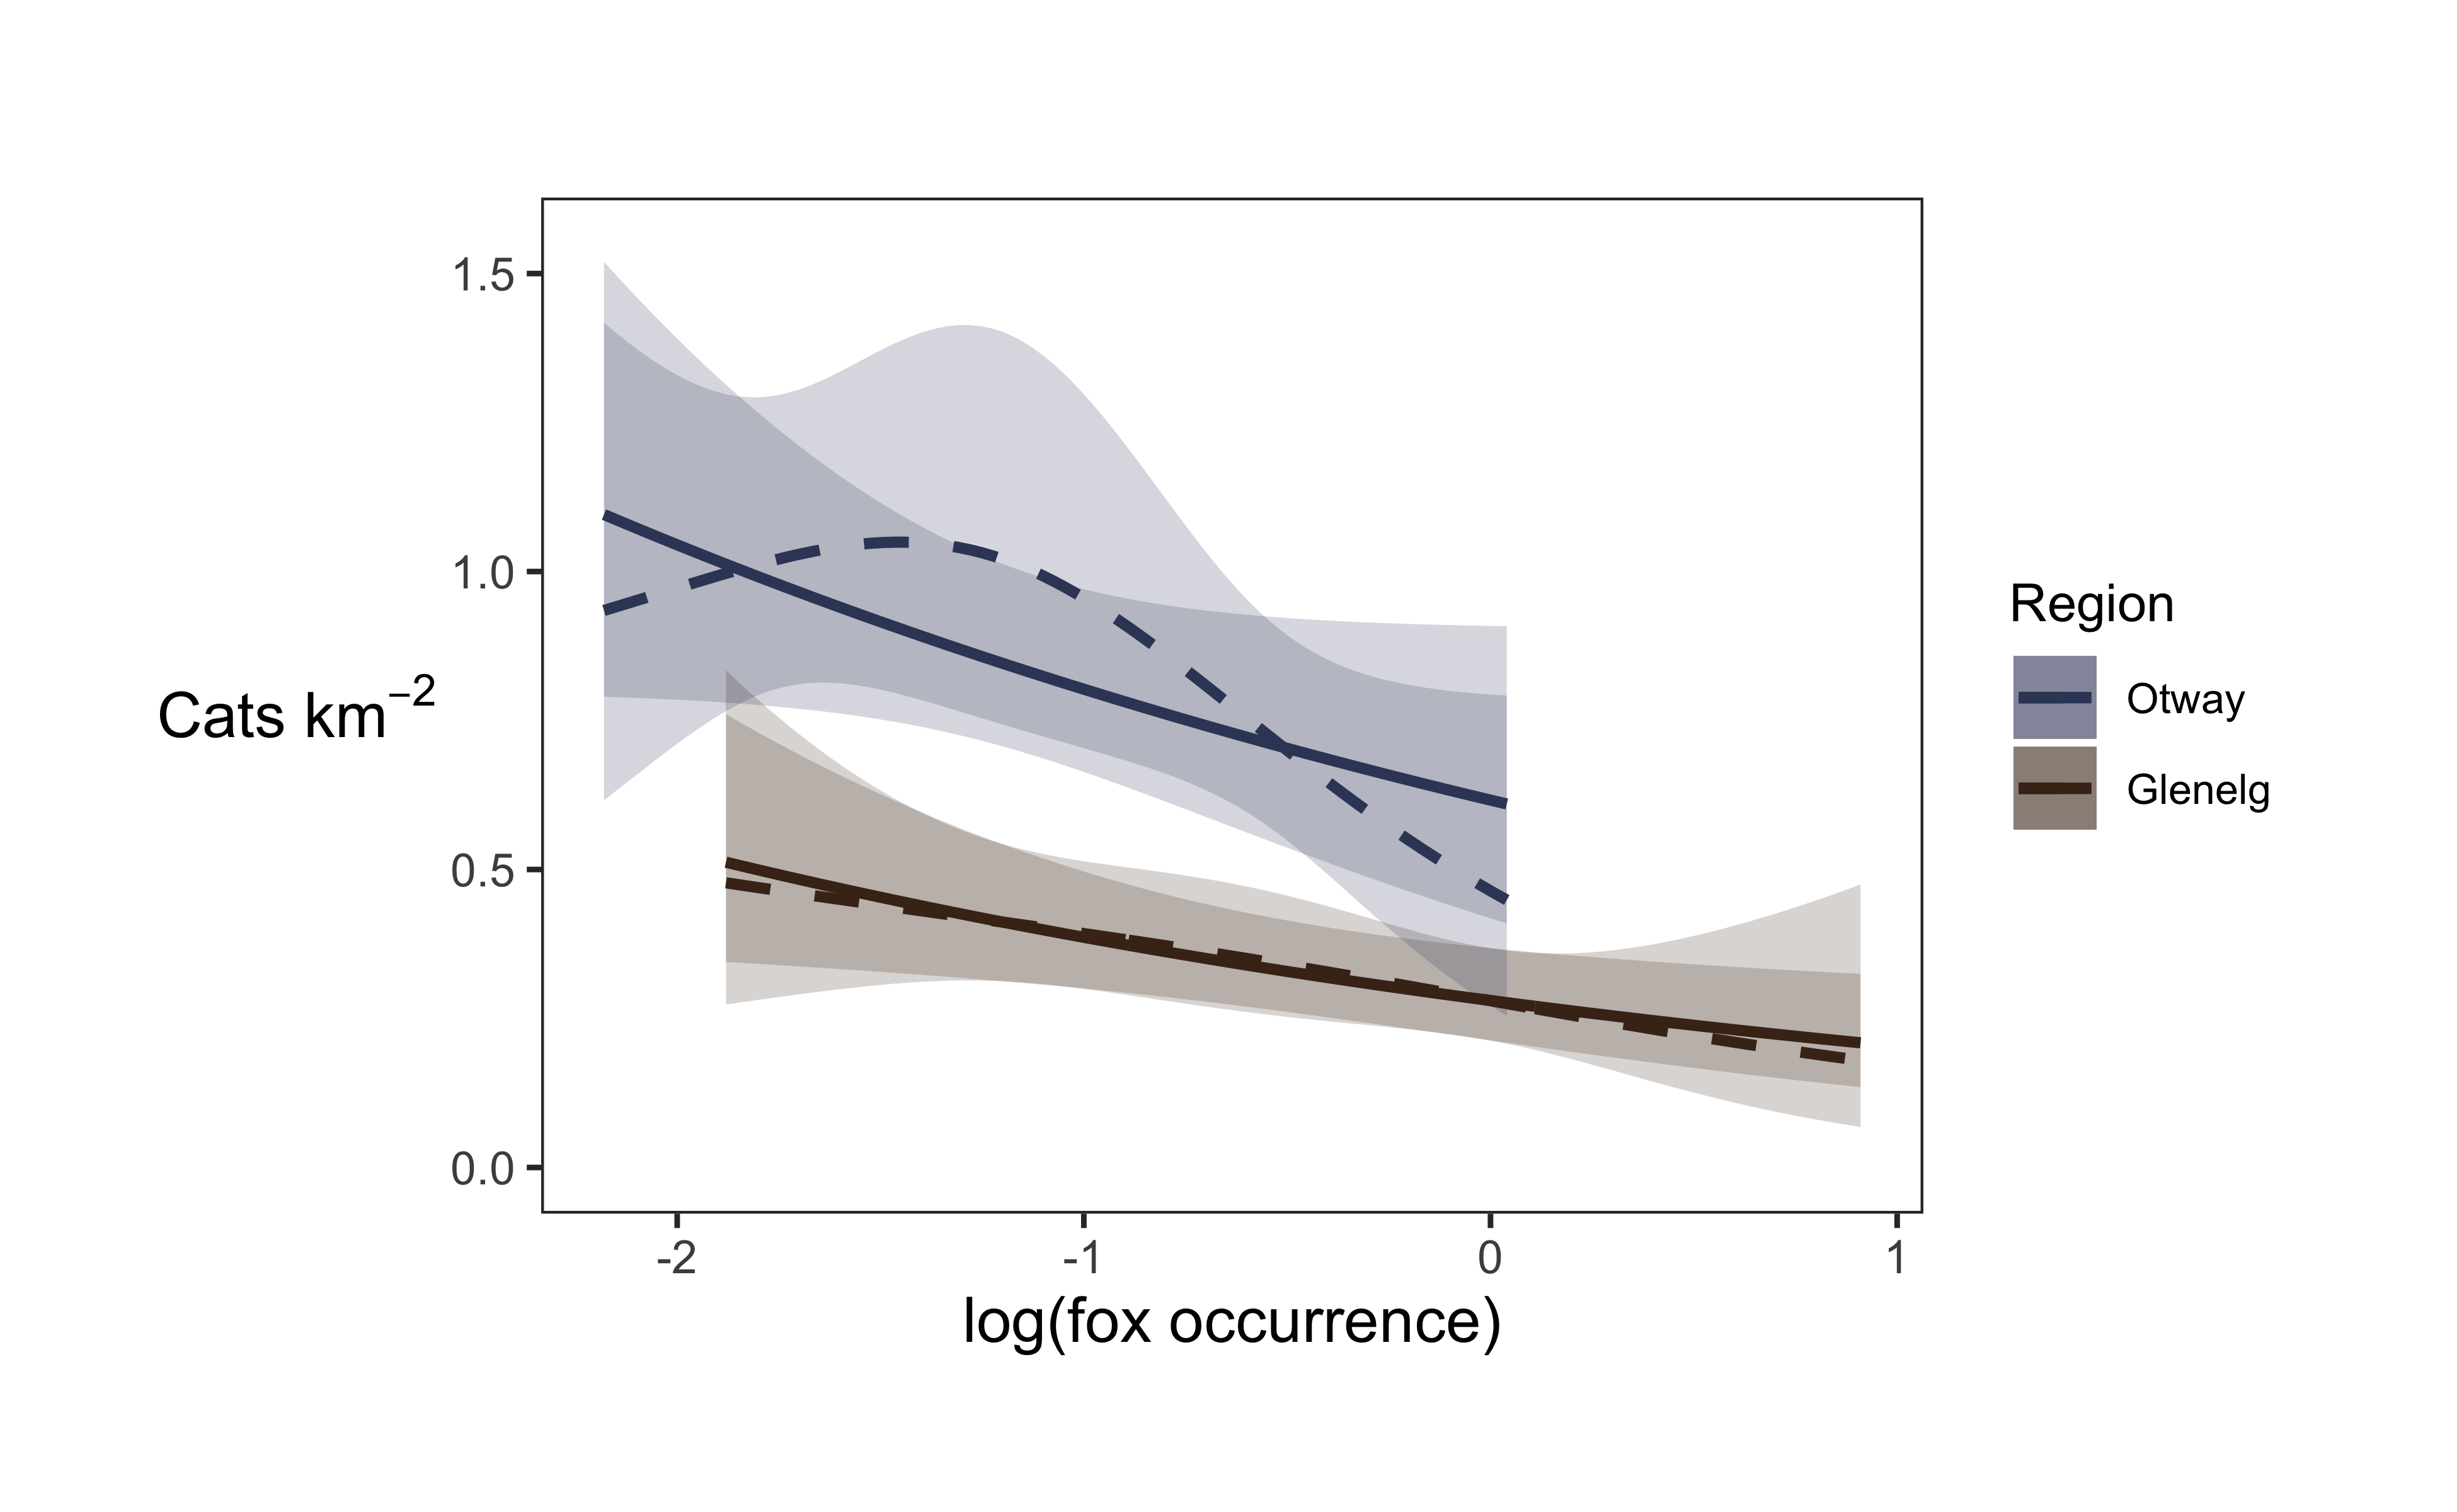
\includegraphics[width=1\linewidth]{figure/c3/foxD_600dpi} 

}

\caption{Linear (solid lines) and nonlinear (dashed lines) models predicted that feral cat \textit{Felis catus} density increased with declining probability of red fox \textit{Vulpes vulpes} occurrence (log-transformed) in the Glenelg and Otway regions, Australia. Shaded areas indicate 95\% confidence intervals.}\label{fig:dcor}
\end{figure}
\newpage

\(~\)

\(~\)

\(~\)
\begin{figure}

{\centering 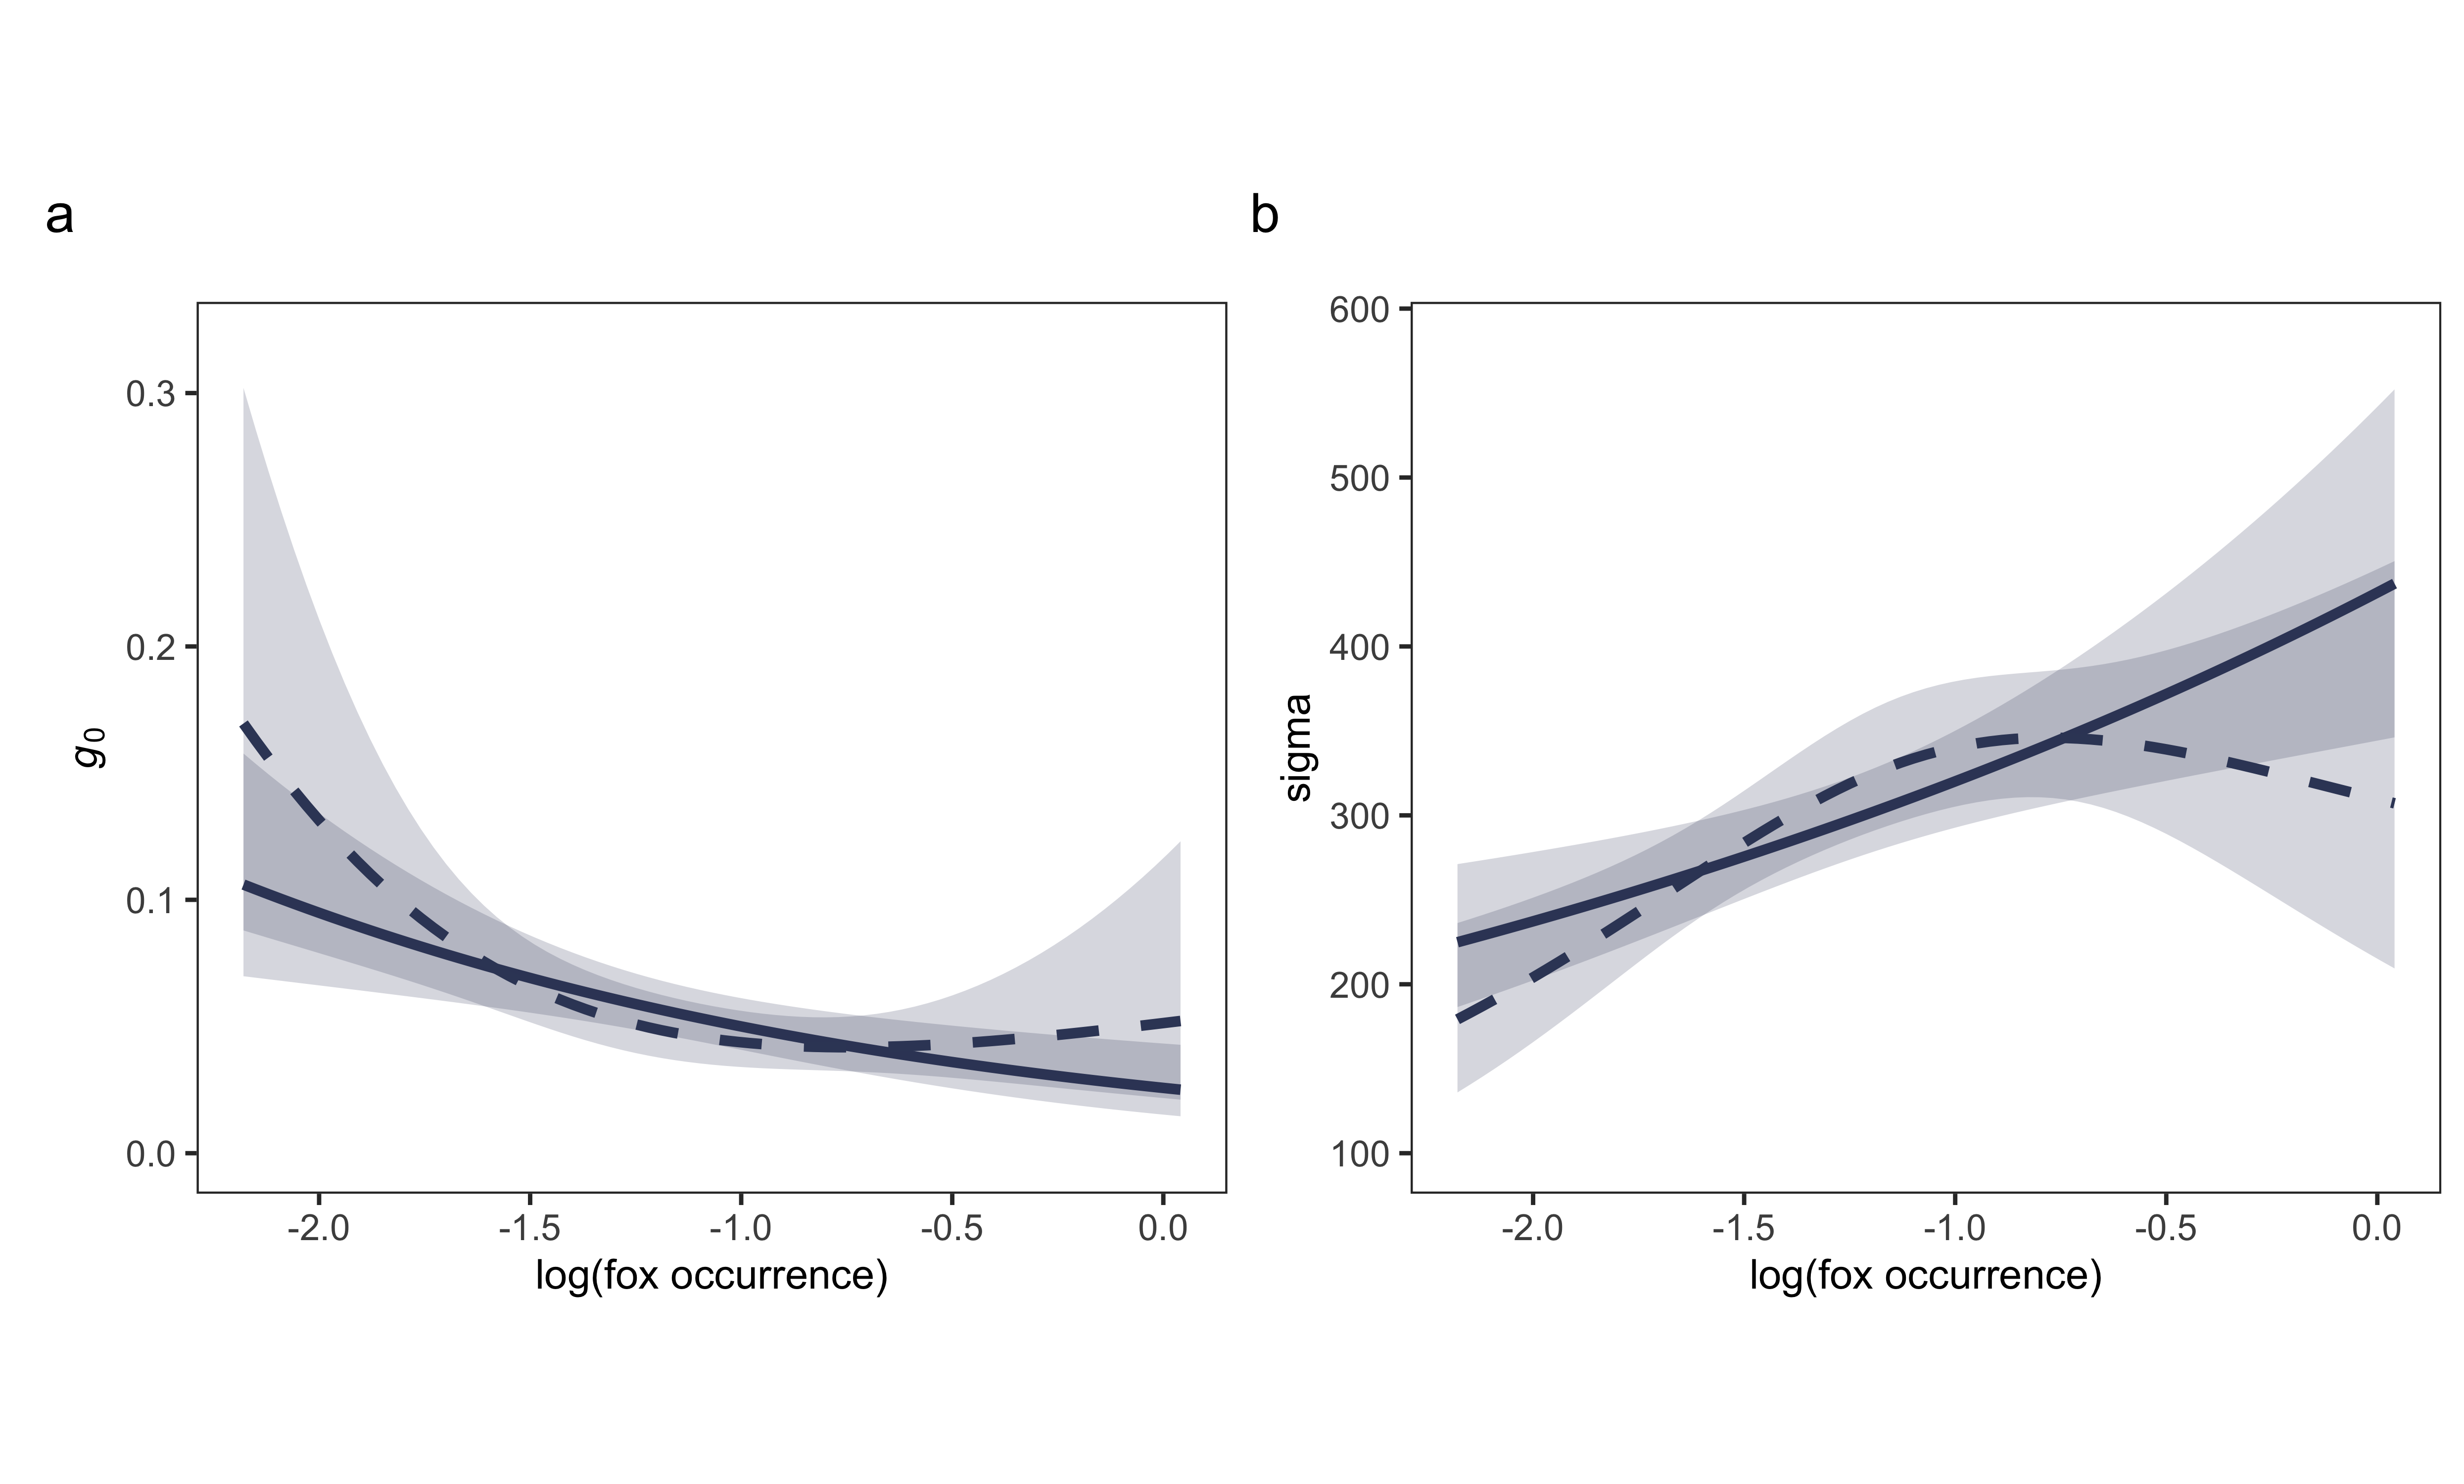
\includegraphics[width=1\linewidth]{figure/c3/foxDet_otways_600dpi} 

}

\caption{Linear (solid lines) and nonlinear (dashed lines) models of feral cat \textit{Felis catus} detectability as a function of log-transformed red fox \textit{Vulpes vulpes} occurrence in the Otway Ranges, Australia. The probability of detecting a feral cat in its activity centre per 24-hour occasion (\textit{g}\textsubscript{0}) decreased with the probability of fox occurrence (a), while sigma (which is related to home range size; exponential detection function) increased (b). Shaded areas indicate 95\% confidence intervals.}\label{fig:detcor}
\end{figure}
\newpage

\(~\)

\(~\)

\(~\)
\begin{figure}

{\centering 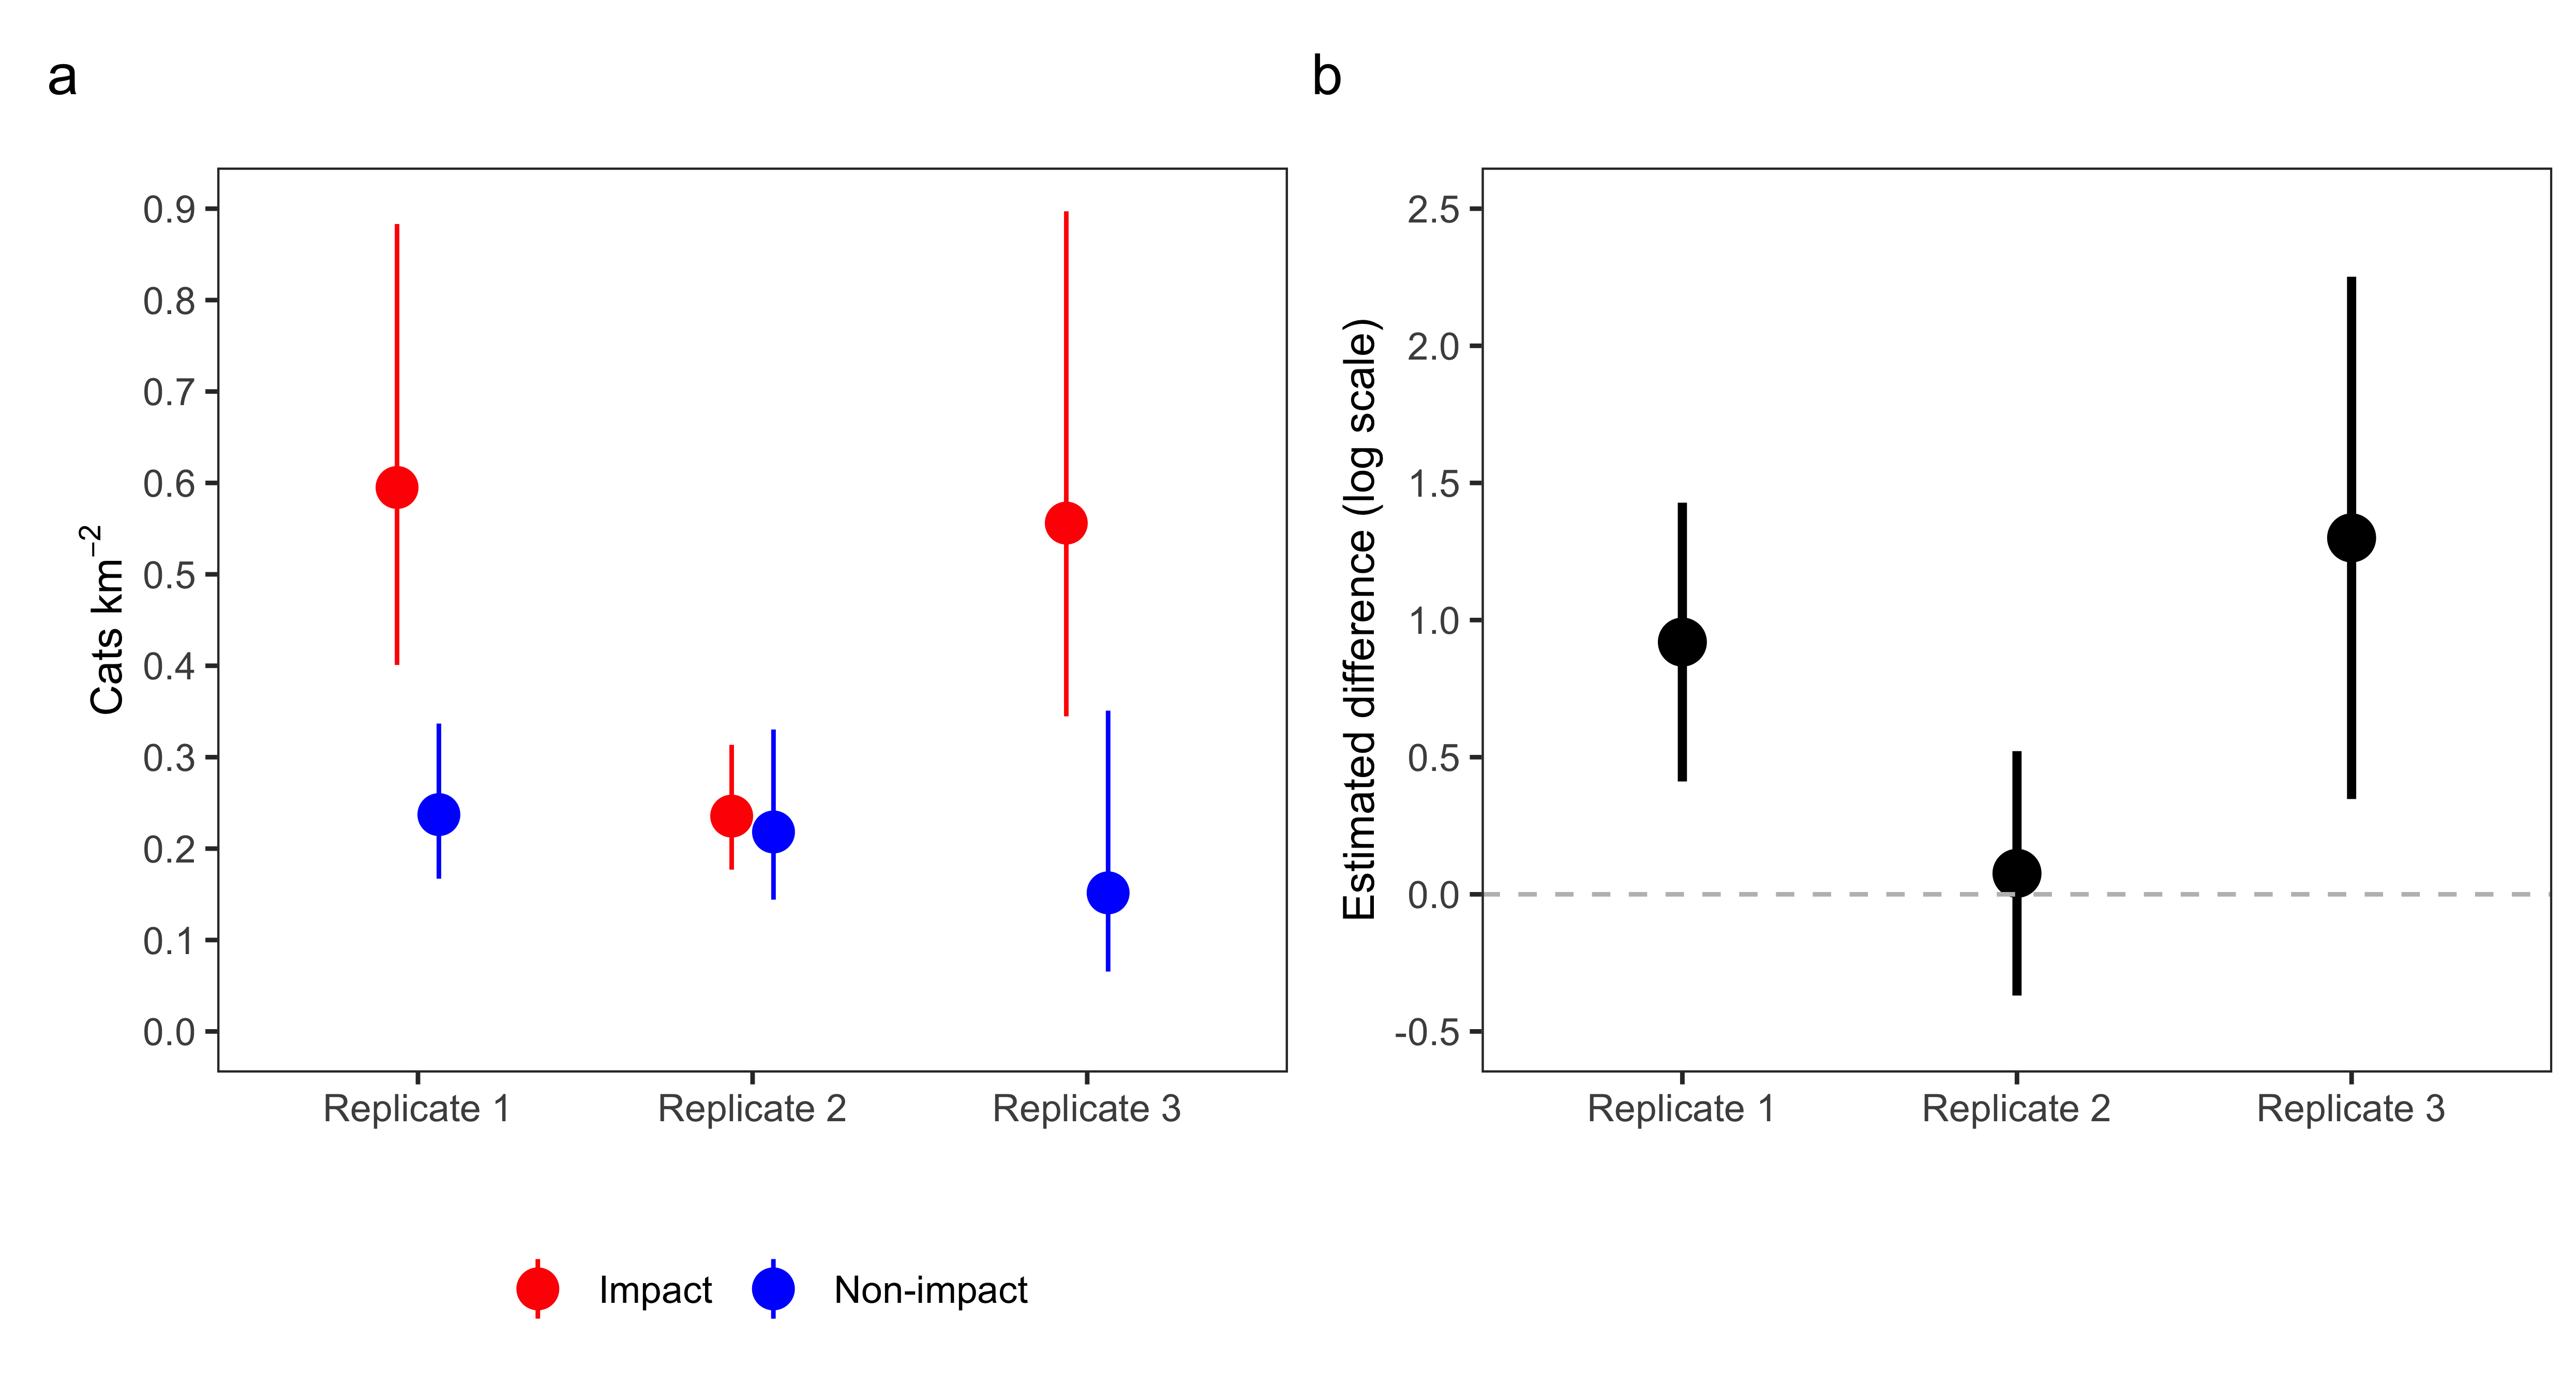
\includegraphics[width=1\linewidth]{figure/c3/glenelg_estimates_600dpi} 

}

\caption{Landscape-scale feral cat \textit{Felis catus} density estimates (a) and response ratio of cat density in the impact landscape relative to the paired non-impact landscape for each replicate (b) in the Glenelg region, Australia. Poison-baiting for foxes \textit{Vulpes vulpes} has been conducted in the impact landscapes for more than 13 years. Grey dashed line represents no difference between the paired landscapes. Error bars represent 95\% confidence intervals.}\label{fig:diffg}
\end{figure}
\newpage

\(~\)

\(~\)

\(~\)
\begin{figure}

{\centering 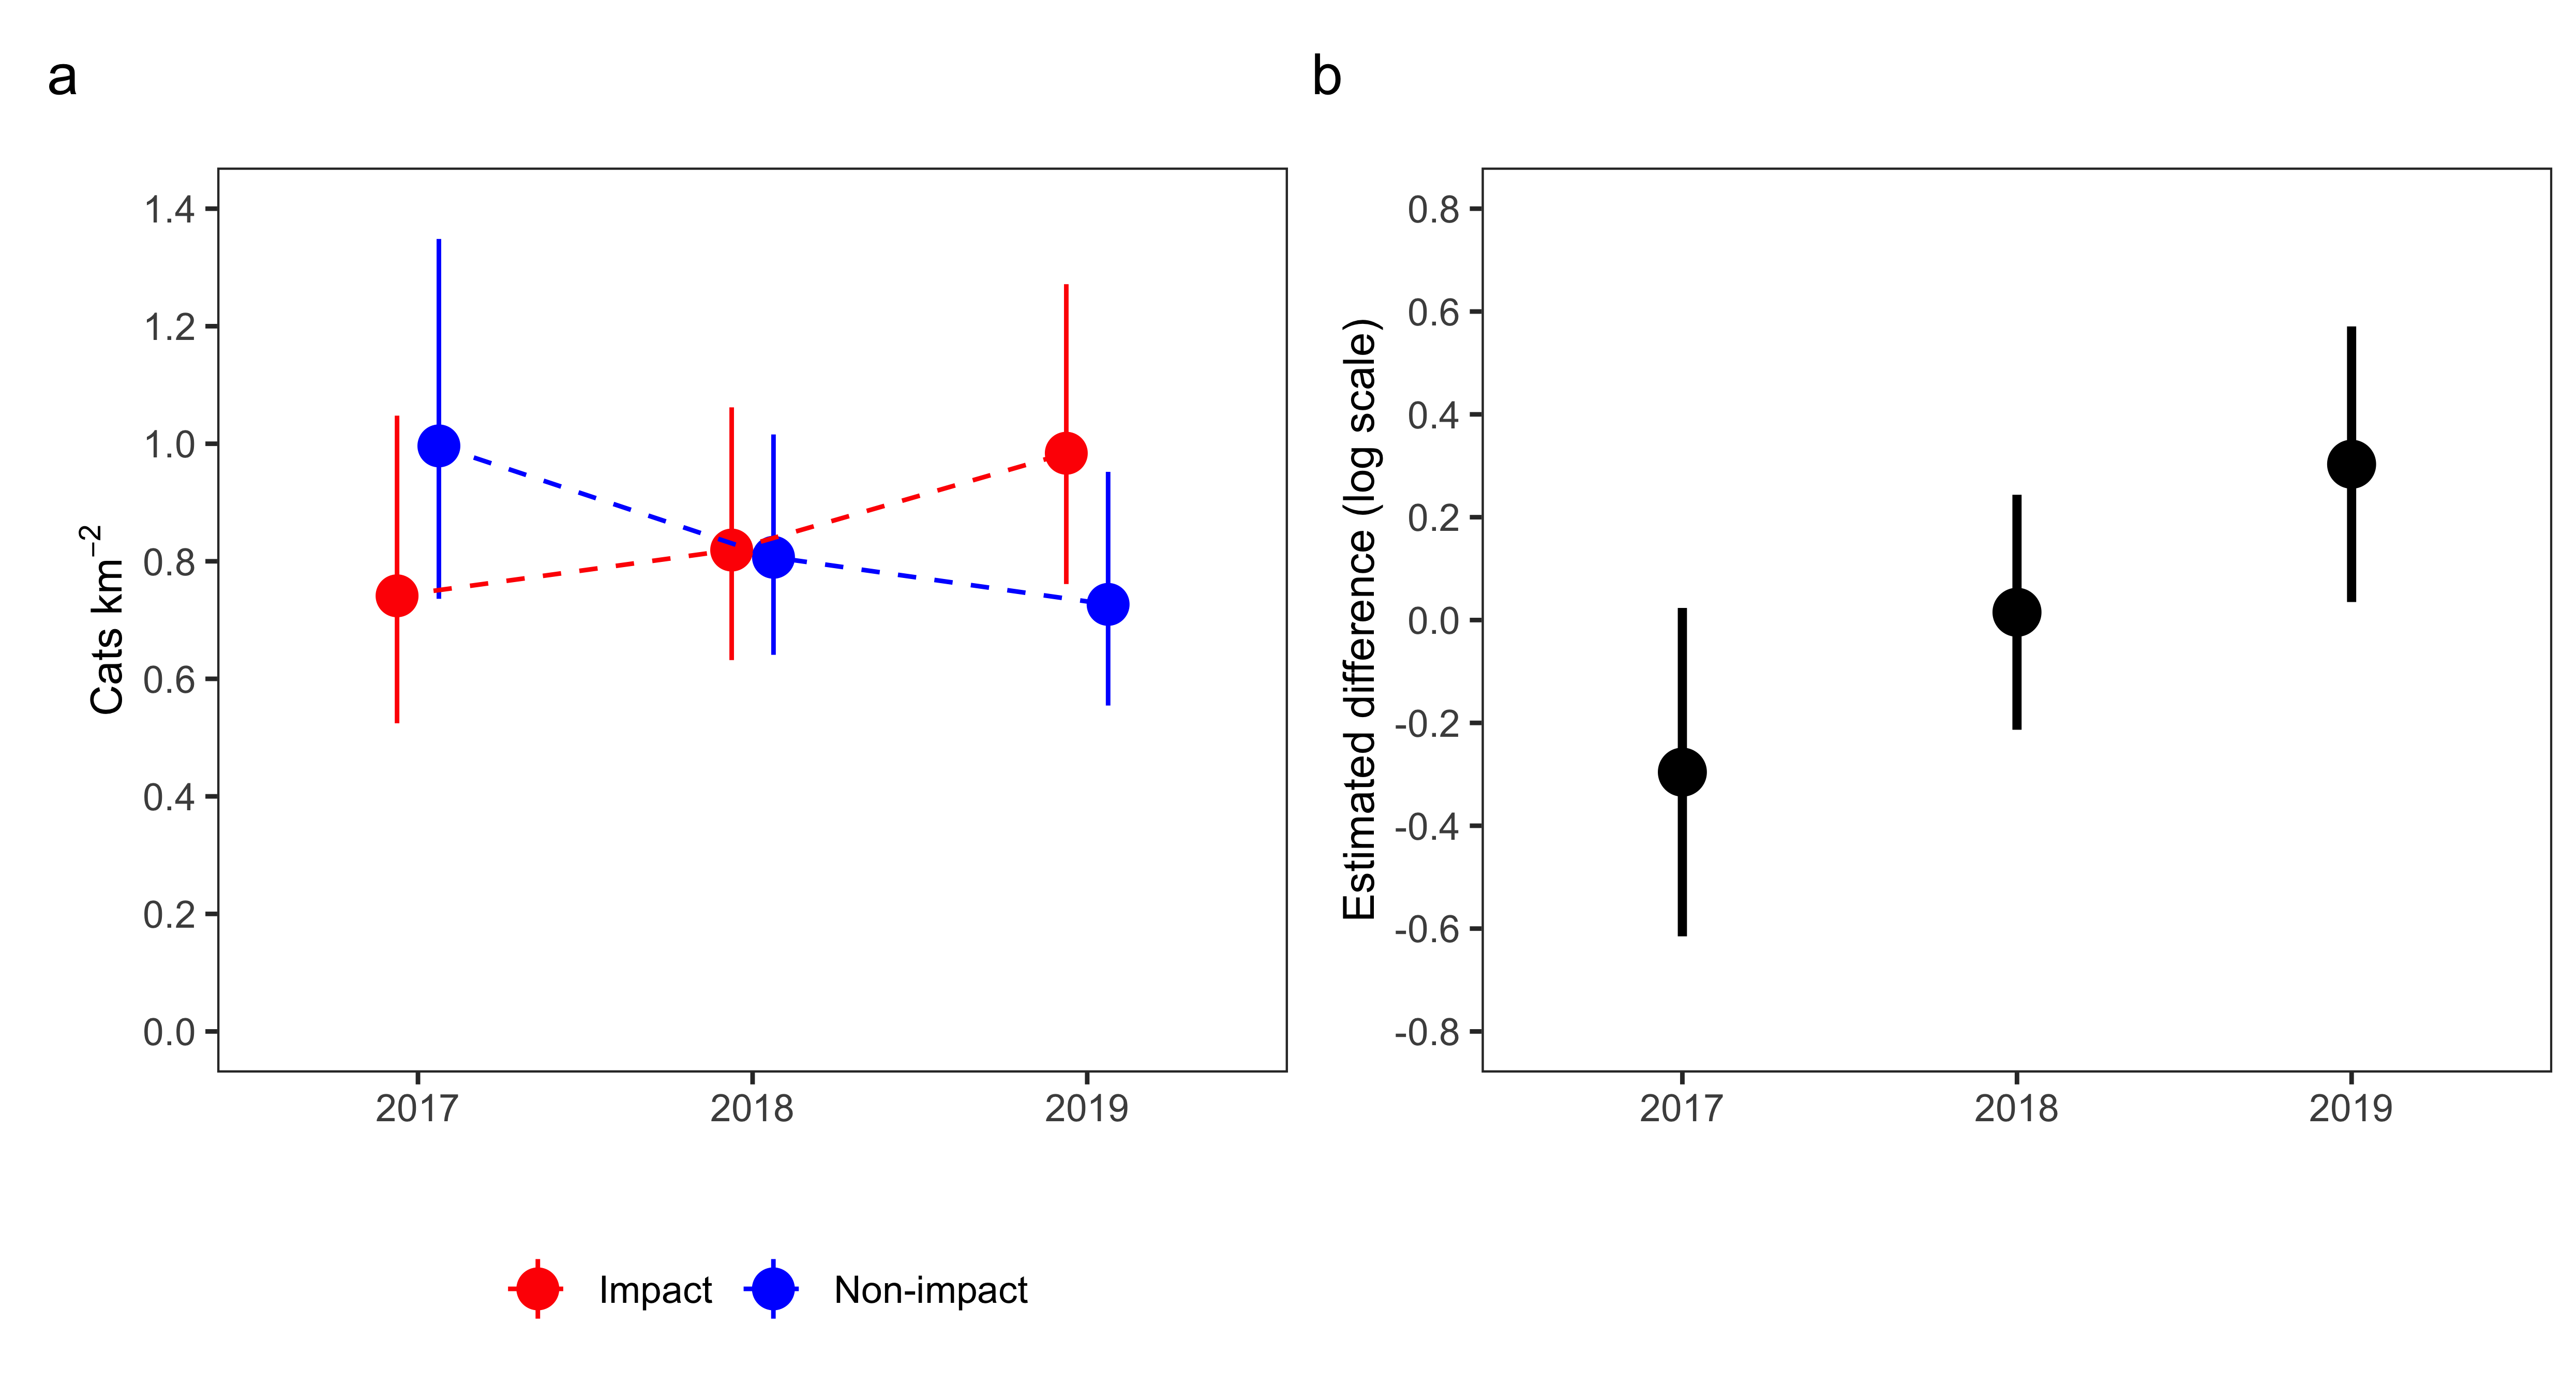
\includegraphics[width=1\linewidth]{figure/c3/otways_estimates_600dpi} 

}

\caption{Landscape-scale feral cat \textit{Felis catus} density estimates (a) and response ratio of cat density in the impact landscape relative to the non-impact landscape for each survey year (b) in the Otway region, Australia. In 2017, surveys were conducted approximately two months before lethal red fox \textit{Vulpes vulpes} control commenced in the impact landscape; control lapsed for six months prior to the 2018 survey. Error bars represent 95\% confidence intervals. Overlap with the grey dashed line in (b) represents no difference in density between the paired landscapes for that year; the proportion overlap between response ratio confidence intervals across years provides evidence for a change in difference.}\label{fig:diffo}
\end{figure}
\newpage

\hypertarget{discussion-3}{%
\section{Discussion}\label{discussion-3}}

Our study is one of the first to provide replicated, experimental evidence that apex predator suppression can increase mesopredator population density. Our study provides two lines of evidence that foxes can exert top-down control on feral cats in the forests of south-eastern Australia: feral cat density was (1) higher where fine-scale fox occurrence probability was lowest, and (2) commonly higher in landscapes where fox control occurred. This is alarming because targeted fox control is a widely used conservation strategy; this unintended consequence could dampen benefits to native prey and even further threaten these species. However, as our findings highlight, mesopredator release of cats following fox control is unlikely to occur universally; the degree of fox suppression varies and fox-cat interactions are likely to be context and scale-dependent. More broadly, our study illustrates how correlative and experimental approaches provide complementary lines of evidence when investigating interactions between predator species, and the importance of disentangling changes in population density from changes in detectability.

We were able to exploit a gradient in fox occurrence caused by lethal control to investigate associations between cat density and fox occurrence at a fine spatial scale across two separate regions. At this scale, we observed a consistently negative association between cat density and fox occurrence, supporting our first hypothesis, although there was more uncertainty around the relationship in the Otway region. We acknowledge that it could also simply reflect differences in niche preference, rather than foxes excluding cats or cats avoiding foxes. However, we consider this unlikely given we observed the relationship across an artificial gradient of fox occurrence caused by lethal control.

There is contention around whether linear regression is appropriate for investigating correlations between different predator species, as subordinate predators may only be suppressed when apex predator abundance is high (Johnson \& VanDerWal 2009). We found no evidence of non-linear associations between foxes and cats in the Glenelg region, while linear and non-linear models performed equally well in the Otway region. Non-linear models in the Otway region predicted that cat density declined only in the mid-high range of fox occurrence, while behavioural changes were seen in the low-mid range of fox occurrence. Perhaps cats can successfully avoid foxes through behavioural change where foxes are rare, but this is ineffective where foxes are common. This could explain the lack of evidence for foxes impacting cat detectability in the Glenelg region where fox occupancy is relatively high. Alternatively, behavioural changes may be untenable for cats in the Glenelg region because small mammal abundance is relatively low and fox avoidance strategies likely come at the expense of hunting success (Sih 1980; Wilson \emph{et al.} 2010).

Where fox occurrence was higher in the Otway Ranges, cats were less detectable in their activity centres and ranged further (Fig. \ref{fig:detcor}). Low detectability is likely to correlate with fewer apex predator encounters, and has been observed in other predator interaction studies (e.g.~Lombardi \emph{et al.} 2017). An increase in cat ranging behaviour (sigma) with fox control supports observations made by Molsher \emph{et al.} (2017), and may reflect a direct avoidance strategy. Animal movement rates are expected to increase in response to unpredictable threats (Riotte-Lambert \& Matthiopoulos 2020). Alternatively, cats may consider foxes predictable and avoid locations they frequent, thus having to range further to obtain the same amount of food resources. In a similar forest habitat, Buckmaster (2012) observed large `holes' in the home range of each GPS-collared cat; they confirmed that this was not due to an absence of prey and hypothesised that it could be due to apex predator avoidance. Regardless of the cause, variation in mesopredator detectability and movement rates with apex predator populations has serious implications for the interpretation of studies that compare relative abundance indices and spatial overlap of predator species without disentangling behaviour and detectability from density (Efford \& Dawson 2012; Neilson \emph{et al.} 2018; Stewart \emph{et al.} 2018; Broadley \emph{et al.} 2019).

In the Glenelg region where fox-baiting had occurred for more than 13 years, feral cat density was considerably higher in two out of three distinct landscapes than in similar, unbaited landscapes. The outlier is most likely due to limited suppression of foxes at Mt Clay despite ongoing fox control (Fig. \ref{fig:foxplot}). Mt Clay is a small forest block surrounded entirely by unbaited farmland. Simulation modelling indicates that the size of the baited area is a key driver of the degree of reduction in the fox population (Hradsky \emph{et al.} 2019; Francis \emph{et al.} 2020). Studies of fox-cat (and other predator-predator) interactions often use the presence of a management program as a proxy for lower apex predator abundance and distribution (e.g.~Hunter \emph{et al.} 2018). Our findings strongly indicate the need to directly measure the apex predator population in order to reliably interpret the responses of subordinate species (Salo \emph{et al.} 2010).

In the Otway region, we observed a weaker--but increasing--effect of fox control on cat density, to be expected from a recently commenced and less intensive fox-baiting program. The short duration of baiting in the Otway region may mean that changes in adult cat density are yet to fully manifest as foxes potentially suppress cats by reducing recruitment rates. Cats may also respond to an increase in shared prey availability following fox suppression (Stobo-Wilson \emph{et al.} 2020). A time-lagged release of cats following fox control would explain eruptions and subsequent crashes commonly observed in shared mammalian prey populations two to ten years following fox control commencement (Duncan \emph{et al.} 2020). Alternatively, top-down suppression by foxes and competition may be weaker in this highly productive environment where prey abundance was relatively high, fox occurrence was already relatively low, and overall cat densities were consistently high (Johnson \& VanDerWal 2009; Greenville \emph{et al.} 2014; Newsome \emph{et al.} 2017). Our surveys provide important baselines against which to compare future changes in predator populations as the fox-baiting program continues.

Our study is among the very few which have used a direct measure of density to test mesopredator release. Previous studies have mostly used live capture-rates to infer population density, without accounting for behavioural or detectability changes (e.g.~Arjo \emph{et al.} 2007; Karki \emph{et al.} 2007; Thompson \& Gese 2007; Berger \emph{et al.} 2008; Jones \emph{et al.} 2008). Contention about mesopredator release has centred on such methods (Hayward \emph{et al.} 2015); as well as unaccounted species interactions in complex predator guilds (Levi \& Wilmers 2012; Jachowski \emph{et al.} 2020). In contrast, our study tests the mesopredator release theory using a combined behavioural and numerical approach, in a system with a simplified carnivore guild. One limitation of our approach is that uncertainty from our fox occurrence models was not propagated into the spatial mark-resight models. A full Bayesian integration of the fox occurrence analysis and the spatial mark-resight model to address this is not yet implemented. The development of open population spatial mark-resight models would also improve parameter estimates for multi-season surveys.

The results of our study may explain why pest management that only targets foxes--one of the most prevalent conservation actions in Australia--does not consistently improve native prey persistence (Dexter \& Murray 2009; Robley \emph{et al.} 2014b; Wayne \emph{et al.} 2017; Lindenmayer \emph{et al.} 2018; Duncan \emph{et al.} 2020). More evidence is required to understand the circumstances in which lethal fox control increases cat density, particularly the role of baseline fox and prey densities. A more integrated approach to invasive predator management, where foxes and cats are simultaneously or otherwise optimally controlled could substantially improve biodiversity outcomes (Risbey \emph{et al.} 2000; Comer \emph{et al.} 2020). If this is not feasible, changes in invasive mesopredator density and the outcomes for native prey species should be closely monitored as part of any control program for invasive apex predators, with triggers for ceasing apex predator control or commencing integrated management if single-species control proves counterproductive for the conservation of threatened prey species.

\hypertarget{synthesis}{%
\chapter*{Synthesis}\label{synthesis}}
\addcontentsline{toc}{chapter}{Synthesis}

text

\hypertarget{references}{%
\chapter*{References}\label{references}}
\addcontentsline{toc}{chapter}{References}

\markboth{References}{References}

\noindent

\setlength{\parindent}{-0.20in}
\setlength{\leftskip}{0.20in}

\hypertarget{refs}{}
\leavevmode\hypertarget{ref-azzou2021sparse}{}%
Ait Kaci Azzou, S., Singer, L., Aebischer, T., Caduff, M., Wolf, B. \& Wegmann, D. (2021). A sparse observation model to quantify species distributions and their overlap in space and time. \emph{Ecography}, 44, 928--940.

\leavevmode\hypertarget{ref-alston2019reciprocity}{}%
Alston, J., Maitland, B., Brito, B., Esmaeili, S., Ford, A. \& Hays, B. \emph{et al.} (2019). Reciprocity in restoration ecology: When might large carnivore reintroduction restore ecosystems? \emph{Biological conservation}, 234, 82--89.

\leavevmode\hypertarget{ref-arjo2007changes}{}%
Arjo, W.M., Gese, E.M., Bennett, T.J. \& Kozlowski, A.J. (2007). Changes in kit fox--coyote--prey relationships in the Great Basin Desert, Utah. \emph{Western North American Naturalist}, 67, 389--401.

\leavevmode\hypertarget{ref-ballari2016potential}{}%
Ballari, S.A., Kuebbing, S.E. \& Nuñez, M.A. (2016). Potential problems of removing one invasive species at a time: A meta-analysis of the interactions between invasive vertebrates and unexpected effects of removal programs. \emph{PeerJ}, 4, e2029.

\leavevmode\hypertarget{ref-banikos2018responses}{}%
Banikos, Z. (2018). Responses of critical weight range digging mammals to a fox control program in south-eastern Australia. Master's thesis. University of Melbourne; School of BioSciences.

\leavevmode\hypertarget{ref-banks1999predation}{}%
Banks, P.B. (1999). Predation by introduced foxes on native bush rats in Australia: Do foxes take the doomed surplus? \emph{Journal of Applied Ecology}, 36, 1063--1071.

\leavevmode\hypertarget{ref-bengsen2011estimating}{}%
Bengsen, A., Butler, J. \& Masters, P. (2011). Estimating and indexing feral cat population abundances using camera traps. \emph{Wildlife Research}, 38, 732--739.

\leavevmode\hypertarget{ref-bengsen2016feral}{}%
Bengsen, A.J., Algar, D., Ballard, G., Buckmaster, T., Comer, S. \& Fleming, P.J.S. \emph{et al.} (2016). Feral cat home-range size varies predictably with landscape productivity and population density. \emph{Journal of Zoology}, 298, 112--120.

\leavevmode\hypertarget{ref-berger2008indirect}{}%
Berger, K.M., Gese, E.M. \& Berger, J. (2008). Indirect effects and traditional trophic cascades: A test involving wolves, coyotes, and pronghorn. \emph{Ecology}, 89, 818--828.

\leavevmode\hypertarget{ref-bilney2010underestimated}{}%
Bilney, R.J., Cooke, R. \& White, J.G. (2010). Underestimated and severe: Small mammal decline from the forests of south-eastern Australia since European settlement, as revealed by a top-order predator. \emph{Biological Conservation}, 143, 52--59.

\leavevmode\hypertarget{ref-maptools}{}%
Bivand, R. \& Lewin-Koh, N. (2021). \emph{Maptools: Tools for handling spatial objects}.

\leavevmode\hypertarget{ref-bode2015eradicating}{}%
Bode, M., Baker, C.M. \& Plein, M. (2015). Eradicating down the food chain: Optimal multispecies eradication schedules for a commonly encountered invaded island ecosystem. \emph{Journal of Applied Ecology}, 52, 571--579.

\leavevmode\hypertarget{ref-borchers2008spatially}{}%
Borchers, D.L. \& Efford, M.G. (2008). Spatially explicit maximum likelihood methods for capture--recapture studies. \emph{Biometrics}, 64, 377--385.

\leavevmode\hypertarget{ref-broadley2019density}{}%
Broadley, K., Burton, A.C., Avgar, T. \& Boutin, S. (2019). Density-dependent space use affects interpretation of camera trap detection rates. \emph{Ecology and evolution}, 9, 14031--14041.

\leavevmode\hypertarget{ref-buckmaster2012ecology}{}%
Buckmaster, A.J. (2012). Ecology of the feral cat \emph{(Felis catus)} in the tall forests of far east gippsland. PhD thesis. University of Sydney.; School of Biological Sciences; University of Sydney.; School of Biological Sciences.

\leavevmode\hypertarget{ref-burbidge2002mammal}{}%
Burbidge, A.A. \& Manly, B.F.J. (2002). Mammal extinctions on Australian islands: Causes and conservation implications. \emph{Journal of Biogeography}, 29, 465--473.

\leavevmode\hypertarget{ref-BOM2021}{}%
Bureau of Meteorology. (2021). Climate data online.

\leavevmode\hypertarget{ref-burnham2004multimodel}{}%
Burnham, K.P. \& Anderson, D.R. (2004). Multimodel inference: Understanding AIC and BIC in model selection. \emph{Sociological methods \& research}, 33, 261--304.

\leavevmode\hypertarget{ref-chandler2013spatially}{}%
Chandler, R.B. \& Royle, J.A. (2013). Spatially explicit models for inference about density in unmarked or partially marked populations. \emph{The Annals of Applied Statistics}, 7, 936--954.

\leavevmode\hypertarget{ref-christie2019simple}{}%
Christie, A.P., Amano, T., Martin, P.A., Shackelford, G.E., Simmons, B.I. \& Sutherland, W.J. (2019). Simple study designs in ecology produce inaccurate estimates of biodiversity responses. \emph{Journal of Applied Ecology}, 56, 2742--2754.

\leavevmode\hypertarget{ref-claridge2010trends}{}%
Claridge, A.W., Cunningham, R.B., Catling, P.C. \& Reid, A.M. (2010). Trends in the activity levels of forest-dwelling vertebrate fauna against a background of intensive baiting for foxes. \emph{Forest Ecology and Management}, 260, 822--832.

\leavevmode\hypertarget{ref-comer2020integrating}{}%
Comer, S., Clausen, L., Cowen, S., Pinder, J., Thomas, A. \& Burbidge, A.H. \emph{et al.} (2020). Integrating feral cat (felis catus) control into landscape-scale introduced predator management to improve conservation prospects for threatened fauna: A case study from the south coast of Western Australia. \emph{Wildlife Research}, 47, 762--778.

\leavevmode\hypertarget{ref-courchamp1999cats}{}%
Courchamp, F., Langlais, M. \& Sugihara, G. (1999). Cats protecting birds: Modelling the mesopredator release effect. \emph{Journal of Animal Ecology}, 68, 282--292.

\leavevmode\hypertarget{ref-cove2018free}{}%
Cove, M.V., Gardner, B., Simons, T.R., Kays, R. \& O'Connell, A.F. (2018). Free-ranging domestic cats \emph{(Felis catus)} on public lands: Estimating density, activity, and diet in the florida keys. \emph{Biological Invasions}, 20, 333--344.

\leavevmode\hypertarget{ref-crooks1999mesopredator}{}%
Crooks, K.R. \& Soulé, M.E. (1999). Mesopredator release and avifaunal extinctions in a fragmented system. \emph{Nature}, 400, 563--566.

\leavevmode\hypertarget{ref-cumming2005inference}{}%
Cumming, G. \& Finch, S. (2005). Inference by eye: Confidence intervals and how to read pictures of data. \emph{American psychologist}, 60, 170.

\leavevmode\hypertarget{ref-davey2006exotic}{}%
Davey, C., Sinclair, A., Pech, R.P., Arthur, A.D., Krebs, C.J. \& Newsome, A. \emph{et al.} (2006). Do exotic vertebrates structure the biota of Australia? An experimental test in new south wales. \emph{Ecosystems}, 9, 992--1008.

\leavevmode\hypertarget{ref-davies2018declining}{}%
Davies, H.F., McCarthy, M.A., Firth, R.S., Woinarski, J.C., Gillespie, G.R. \& Andersen, A.N. \emph{et al.} (2018). Declining populations in one of the last refuges for threatened mammal species in northern Australia. \emph{Austral Ecology}, 43, 602--612.

\leavevmode\hypertarget{ref-delwp2020}{}%
DELWP. (2020). \emph{Bioregions and evc benchmarks}. Available at: \url{https://www.environment.vic.gov.au/biodiversity/bioregions-and-evc-benchmarks}. Last accessed.

\leavevmode\hypertarget{ref-denny2010review}{}%
Denny, E.A. \& Dickman, C. (2010). Review of cat ecology and management strategies in Australia. \emph{Invasive Animals Cooperative Research Centre, Canberra}.

\leavevmode\hypertarget{ref-dexter2009impact}{}%
Dexter, N. \& Murray, A. (2009). The impact of fox control on the relative abundance of forest mammals in east gippsland, victoria. \emph{Wildlife Research}, 36, 252--261.

\leavevmode\hypertarget{ref-dickman1996overview}{}%
Dickman, C.R. (1996). \emph{Overview of the impacts of feral cats on Australian native fauna}. Australian Nature Conservation Agency Canberra.

\leavevmode\hypertarget{ref-doherty2015critical}{}%
Doherty, T.S., Bengsen, A.J. \& Davis, R.A. (2015). A critical review of habitat use by feral cats and key directions for future research and management. \emph{Wildlife Research}, 41, 435--446.

\leavevmode\hypertarget{ref-doherty2017impacts}{}%
Doherty, T.S., Dickman, C.R., Johnson, C.N., Legge, S.M., Ritchie, E.G. \& Woinarski, J.C. (2017). Impacts and management of feral cats \emph{(Felis catus)} in Australia. \emph{Mammal Review}, 47, 83--97.

\leavevmode\hypertarget{ref-doherty2019conservation}{}%
Doherty, T.S., Driscoll, D.A., Nimmo, D.G., Ritchie, E.G. \& Spencer, R.-J. (2019). Conservation or politics? Australia's target to kill 2 million cats. \emph{Conservation Letters}, 12, e12633.

\leavevmode\hypertarget{ref-doherty2017stop}{}%
Doherty, T.S. \& Ritchie, E.G. (2017). Stop jumping the gun: A call for evidence-based invasive predator management. \emph{Conservation Letters}, 10, 15--22.

\leavevmode\hypertarget{ref-duncan2020eruptive}{}%
Duncan, R.P., Dexter, N., Wayne, A. \& Hone, J. (2020). Eruptive dynamics are common in managed mammal populations. \emph{Ecology}, 101, e03175.

\leavevmode\hypertarget{ref-edwards2000evaluation}{}%
Edwards, G., De Preu, N., Shakeshaft, B. \& Crealy, I. (2000). An evaluation of two methods of assessing feral cat and dingo abundance in central Australia. \emph{Wildlife Research}, 27, 143--149.

\leavevmode\hypertarget{ref-efford2021secr}{}%
Efford, M.G. (2021). \emph{Secr: Spatially explicit capture-recapture models. R package version 4.4.4}. Available at: \url{http://CRAN.R-project.org/package=secr}. Last accessed.

\leavevmode\hypertarget{ref-efford2012occupancy}{}%
Efford, M.G. \& Dawson, D.K. (2012). Occupancy in continuous habitat. \emph{Ecosphere}, 3, 1--15.

\leavevmode\hypertarget{ref-efford2018spatial}{}%
Efford, M.G. \& Hunter, C.M. (2018). Spatial capture--mark--resight estimation of animal population density. \emph{Biometrics}, 74, 411--420.

\leavevmode\hypertarget{ref-efford2014compensatory}{}%
Efford, M.G. \& Mowat, G. (2014). Compensatory heterogeneity in spatially explicit capture--recapture data. \emph{Ecology}, 95, 1341--1348.

\leavevmode\hypertarget{ref-elmhagen2007trophic}{}%
Elmhagen, B. \& Rushton, S.P. (2007). Trophic control of mesopredators in terrestrial ecosystems: Top-down or bottom-up? \emph{Ecology Letters}, 10, 197--206.

\leavevmode\hypertarget{ref-farris2020exploring}{}%
Farris, Z.J., Gerber, B.D., Karpanty, S., Murphy, A., Wampole, E. \& Ratelolahy, F. \emph{et al.} (2020). Exploring and interpreting spatiotemporal interactions between native and invasive carnivores across a gradient of rainforest degradation. \emph{Biological Invasions}, 22, 2033--2047.

\leavevmode\hypertarget{ref-finke2004predator}{}%
Finke, D.L. \& Denno, R.F. (2004). Predator diversity dampens trophic cascades. \emph{Nature}, 429, 407--410.

\leavevmode\hypertarget{ref-fisher2014current}{}%
Fisher, D.O., Johnson, C.N., Lawes, M.J., Fritz, S.A., McCallum, H. \& Blomberg, S.P. \emph{et al.} (2014). The current decline of tropical marsupials in Australia: Is history repeating? \emph{Global Ecology and Biogeography}, 23, 181--190.

\leavevmode\hypertarget{ref-fisher2015cat}{}%
Fisher, P., Algar, D., Murphy, E., Johnston, M. \& Eason, C. (2015). How does cat behaviour influence the development and implementation of monitoring techniques and lethal control methods for feral cats? \emph{Applied Animal Behaviour Science}, 173, 88--96.

\leavevmode\hypertarget{ref-francis2020evaluating}{}%
Francis, L., Robley, A. \& Hradsky, B. (2020). \emph{Evaluating fox management strategies using a spatially explicit population}. Arthur Rylah Institute for Environmental Research Technical Report Series No. 304. Department of Environment, Land, Water; Planning, Heidelberg, Victoria.

\leavevmode\hypertarget{ref-frey2017investigating}{}%
Frey, S., Fisher, J.T., Burton, A.C. \& Volpe, J.P. (2017). Investigating animal activity patterns and temporal niche partitioning using camera-trap data: Challenges and opportunities. \emph{Remote Sensing in Ecology and Conservation}, 3, 123--132.

\leavevmode\hypertarget{ref-https:ux2fux2fdoi.orgux2f10.1111ux2fj.1442-9993.2008.01869.x}{}%
Garrard, G.E., Bekkessy, S.A., McCarthy, M.A. \& Wintle, B.A. (2008). When have we looked hard enough? A novel method for setting minimum survey effort protocols for flora surveys. \emph{Austral Ecology}, 33, 986--998.

\leavevmode\hypertarget{ref-glen2005complex}{}%
Glen, A.S. \& Dickman, C.R. (2005). Complex interactions among mammalian carnivores in Australia, and their implications for wildlife management. \emph{Biological reviews}, 80, 387--401.

\leavevmode\hypertarget{ref-greenville2014bottom}{}%
Greenville, A.C., Wardle, G.M., Tamayo, B. \& Dickman, C.R. (2014). Bottom-up and top-down processes interact to modify intraguild interactions in resource-pulse environments. \emph{Oecologia}, 175, 1349--1358.

\leavevmode\hypertarget{ref-https:ux2fux2fdoi.orgux2f10.1111ux2fddi.12471}{}%
Hale, S., Nimmo, D.G., Cooke, R., Holland, G., James, S. \& Stevens, M. \emph{et al.} (2016). Fire and climatic extremes shape mammal distributions in a fire-prone landscape. \emph{Diversity and Distributions}, 22, 1127--1138.

\leavevmode\hypertarget{ref-DHARMa}{}%
Hartig, F. (2020). \emph{DHARMa: Residual diagnostics for hierarchical (multi-level / mixed) regression models}.

\leavevmode\hypertarget{ref-hastings2001transient}{}%
Hastings, A. (2001). Transient dynamics and persistence of ecological systems. \emph{Ecology Letters}, 4, 215--220.

\leavevmode\hypertarget{ref-hayward2015ecologists}{}%
Hayward, M.W., Boitani, L., Burrows, N.D., Funston, P.J., Karanth, K.U. \& MacKenzie, D.I. \emph{et al.} (2015). Ecologists need robust survey designs, sampling and analytical methods. \emph{Journal of Applied Ecology}, 52, 286--290.

\leavevmode\hypertarget{ref-hohnen2016occupancy}{}%
Hohnen, R., Tuft, K., McGregor, H.W., Legge, S., Radford, I.J. \& Johnson, C.N. (2016). Occupancy of the invasive feral cat varies with habitat complexity. \emph{PLoS One}, 11, e0152520.

\leavevmode\hypertarget{ref-hradsky2019foxnet}{}%
Hradsky, B.A., Kelly, L.T., Robley, A. \& Wintle, B.A. (2019). FoxNet: An individual-based model framework to support management of an invasive predator, the red fox. \emph{Journal of Applied Ecology}, 56, 1460--1470.

\leavevmode\hypertarget{ref-hradsky2017human}{}%
Hradsky, B.A., Robley, A., Alexander, R., Ritchie, E.G., York, A. \& Di Stefano, J. (2017). Human-modified habitats facilitate forest-dwelling populations of an invasive predator, \emph{(Vulpes vulpes)}. \emph{Scientific Reports}, 7, 1--12.

\leavevmode\hypertarget{ref-hunter2018not}{}%
Hunter, D.O., Lagisz, M., Leo, V., Nakagawa, S. \& Letnic, M. (2018). Not all predators are equal: A continent-scale analysis of the effects of predator control on Australian mammals. \emph{Mammal Review}, 48, 108--122.

\leavevmode\hypertarget{ref-iannarilli2019lorelograms}{}%
Iannarilli, F., Arnold, T.W., Erb, J. \& Fieberg, J.R. (2019). Using lorelograms to measure and model correlation in binary data: Applications to ecological studies. \emph{Methods in Ecology and Evolution}, 10, 2153--2162.

\leavevmode\hypertarget{ref-jachowski2020identifying}{}%
Jachowski, D.S., Butler, A., Eng, R.Y.Y., Gigliotti, L., Harris, S. \& Williams, A. (2020). Identifying mesopredator release in multi-predator systems: A review of evidence from north america. \emph{Mammal Review}, 50, 367--381.

\leavevmode\hypertarget{ref-jackson2015interactions}{}%
Jackson, M.C. (2015). Interactions among multiple invasive animals. \emph{Ecology}, 96, 2035--2041.

\leavevmode\hypertarget{ref-jimenez2017estimating}{}%
Jiménez, J., Nuñez-Arjona, J.C., Rueda, C., González, L.M., García-Domínguez, F. \& Muñoz-Igualada, J. \emph{et al.} (2017). Estimating carnivore community structures. \emph{Scientific reports}, 7, 1--10.

\leavevmode\hypertarget{ref-johnson2006australia}{}%
Johnson, C. (2006). \emph{Australia's mammal extinctions: A 50,000-year history}. Cambridge University Press.

\leavevmode\hypertarget{ref-johnson2007rarity}{}%
Johnson, C.N., Isaac, J.L. \& Fisher, D.O. (2007). Rarity of a top predator triggers continent-wide collapse of mammal prey: Dingoes and marsupials in Australia. \emph{Proceedings of the Royal Society B: Biological Sciences}, 274, 341--346.

\leavevmode\hypertarget{ref-johnson2009evidence}{}%
Johnson, C.N. \& VanDerWal, J. (2009). Evidence that dingoes limit abundance of a mesopredator in eastern Australian forests. \emph{Journal of Applied Ecology}, 46, 641--646.

\leavevmode\hypertarget{ref-jones2008sudden}{}%
Jones, K.L., Van Vuren, D.H. \& Crooks, K.R. (2008). Sudden Increase in a Rare Endemic Carnivore: Ecology of the Island Spotted Skunk. \emph{Journal of Mammalogy}, 89, 75--86.

\leavevmode\hypertarget{ref-karki2007effects}{}%
Karki, S.M., Gese, E.M. \& Klavetter, M.L. (2007). Effects of coyote population reduction on swift fox demographics in southeastern colorado. \emph{The Journal of Wildlife Management}, 71, 2707--2718.

\leavevmode\hypertarget{ref-kuebbing2015negative}{}%
Kuebbing, S.E. \& Nuñez, M.A. (2015). Negative, neutral, and positive interactions among nonnative plants: Patterns, processes, and management implications. \emph{Global Change Biology}, 21, 926--934.

\leavevmode\hypertarget{ref-lazenby2015effects}{}%
Lazenby, B.T., Mooney, N.J. \& Dickman, C.R. (2015). Effects of low-level culling of feral cats in open populations: A case study from the forests of southern tasmania. \emph{Wildlife Research}, 41, 407--420.

\leavevmode\hypertarget{ref-legge2017enumerating}{}%
Legge, S., Murphy, B.P., McGregor, H., Woinarski, J.C.Z., Augusteyn, J. \& Ballard, G. \emph{et al.} (2017). Enumerating a continental-scale threat: How many feral cats are in australia? \emph{Biological Conservation}, 206, 293--303.

\leavevmode\hypertarget{ref-legge2020cat}{}%
Legge, S., Taggart, P.L., Dickman, C.R., Read, J.L. \& Woinarski, J.C. (2020). \emph{Wildlife Research}, 47, 731--746.

\leavevmode\hypertarget{ref-levi2012wolves}{}%
Levi, T. \& Wilmers, C.C. (2012). Wolves--coyotes--foxes: A cascade among carnivores. \emph{Ecology}, 93, 921--929.

\leavevmode\hypertarget{ref-lindenmayer2018conservation}{}%
Lindenmayer, D.B., Wood, J., MacGregor, C., Foster, C., Scheele, B. \& Tulloch, A. \emph{et al.} (2018). Conservation conundrums and the challenges of managing unexplained declines of multiple species. \emph{Biological Conservation}, 221, 279--292.

\leavevmode\hypertarget{ref-lombardi2017coyote}{}%
Lombardi, J.V., Comer, C.E., Scognamillo, D.G. \& Conway, W.C. (2017). Coyote, fox, and bobcat response to anthropogenic and natural landscape features in a small urban area. \emph{Urban Ecosystems}, 20, 1239--1248.

\leavevmode\hypertarget{ref-marlow2015cats}{}%
Marlow, N.J., Thomas, N.D., Williams, A.A., Macmahon, B., Lawson, J. \& Hitchen, Y. \emph{et al.} (2015). Cats \emph{(Felis catus)} are more abundant and are the dominant predator of woylies (bettongia penicillata) after sustained fox \emph{(Vulpes vulpes)} control. \emph{Australian Journal of Zoology}, 63, 18--27.

\leavevmode\hypertarget{ref-marra2011practical}{}%
Marra, G. \& Wood, S.N. (2011). Practical variable selection for generalized additive models. \emph{Computational Statistics \& Data Analysis}, 55, 2372--2387.

\leavevmode\hypertarget{ref-MCCOLLGAUSDEN2019243}{}%
McColl-Gausden, S.C. \& Penman, T.D. (2019). Pathways of change: Predicting the effects of fire on flammability. \emph{Journal of Environmental Management}, 232, 243--253.

\leavevmode\hypertarget{ref-mcdonald2017habitat}{}%
McDonald, P.J., Nano, C.E.M., Ward, S.J., Stewart, A., Pavey, C.R. \& Luck, G.W. \emph{et al.} (2017). Habitat as a mediator of mesopredator-driven mammal extinction. \emph{Conservation Biology}, 31, 1183--1191.

\leavevmode\hypertarget{ref-mcgregor2017habitat}{}%
McGregor, H.W., Cliff, H.B. \& Kanowski, J. (2017). Habitat preference for fire scars by feral cats in Cape York Peninsula, Australia. \emph{Wildlife Research}, 43, 623--633.

\leavevmode\hypertarget{ref-mcgregor2014landscape}{}%
McGregor, H.W., Legge, S., Jones, M.E. \& Johnson, C.N. (2014). Landscape management of fire and grazing regimes alters the fine-scale habitat utilisation by feral cats. \emph{PloS one}, 9, e109097.

\leavevmode\hypertarget{ref-mcgregor2015density}{}%
McGregor, H.W., Legge, S., Potts, J., Jones, M.E. \& Johnson, C.N. (2015). Density and home range of feral cats in north-western Australia. \emph{Wildlife Research}, 42, 223--231.

\leavevmode\hypertarget{ref-mcleod2014fertility}{}%
McLeod, S.R. \& Saunders, G. (2014). Fertility control is much less effective than lethal baiting for controlling foxes. \emph{Ecological Modelling}, 273, 1--10.

\leavevmode\hypertarget{ref-medina2011global}{}%
Medina, F.M., Bonnaud, E., Vidal, E., Tershy, B.R., Zavaleta, E.S. \& Josh Donlan, C. \emph{et al.} (2011). A global review of the impacts of invasive cats on island endangered vertebrates. \emph{Global Change Biology}, 17, 3503--3510.

\leavevmode\hypertarget{ref-menkhorst2006background}{}%
Menkhorst, P. \& Broome, L. (2006). \emph{Background and implementation information for the smoky mouse Pseudomys fumeus: National recovery plan}. Department of Sustainability; Environment.

\leavevmode\hypertarget{ref-miller2014finite}{}%
Miller, D.L. \& Wood, S.N. (2014). Finite area smoothing with generalized distance splines. \emph{Environmental and ecological statistics}, 21, 715--731.

\leavevmode\hypertarget{ref-molsher2017mesopredator}{}%
Molsher, R., Newsome, A.E., Newsome, T.M. \& Dickman, C.R. (2017). Mesopredator management: Effects of red fox control on the abundance, diet and use of space by feral cats. \emph{PLoS One}, 12, e0168460.

\leavevmode\hypertarget{ref-moseby2019understanding}{}%
Moseby, K.E., Letnic, M., Blumstein, D.T. \& West, R. (2019). Understanding predator densities for successful co-existence of alien predators and threatened prey. \emph{Austral Ecology}, 44, 409--419.

\leavevmode\hypertarget{ref-moseby2020effectiveness}{}%
Moseby, K., McGregor, H. \& Read, J. (2020). Effectiveness of the felixer grooming trap for the control of feral cats: A field trial in arid South Australia. \emph{Wildlife Research}, 47, 599--609.

\leavevmode\hypertarget{ref-murphy2019introduced}{}%
Murphy, B.P., Woolley, L.-A., Geyle, H.M., Legge, S.M., Palmer, R. \& Dickman, C.R. \emph{et al.} (2019). Introduced cats \emph{(Felis catus)} eating a continental fauna: The number of mammals killed in Australia. \emph{Biological Conservation}, 237, 28--40.

\leavevmode\hypertarget{ref-neilson2018animal}{}%
Neilson, E.W., Avgar, T., Burton, A.C., Broadley, K. \& Boutin, S. (2018). Animal movement affects interpretation of occupancy models from camera-trap surveys of unmarked animals. \emph{Ecosphere}, 9, e02092.

\leavevmode\hypertarget{ref-newsome2017top}{}%
Newsome, T.M., Greenville, A.C., Ćirović, D., Dickman, C.R., Johnson, C.N. \& Krofel, M. \emph{et al.} (2017). Top predators constrain mesopredator distributions. \emph{Nature communications}, 8, 1--7.

\leavevmode\hypertarget{ref-niedballa2016}{}%
Niedballa, J., Sollmann, R., Courtiol, A. \& Wilting, A. (2016). CamtrapR: An r package for efficient camera trap data management. \emph{Methods in Ecology and Evolution}, 7, 1457--1462.

\leavevmode\hypertarget{ref-pedersen2019hierarchical}{}%
Pedersen, E.J., Miller, D.L., Simpson, G.L. \& Ross, N. (2019). Hierarchical generalized additive models in ecology: An introduction with mgcv. \emph{PeerJ}, 7, e6876.

\leavevmode\hypertarget{ref-radford2018degrees}{}%
Radford, J.Q., Woinarski, J.C., Legge, S., Baseler, M., Bentley, J. \& Burbidge, A.A. \emph{et al.} (2018). Degrees of population-level susceptibility of Australian terrestrial non-volant mammal species to predation by the introduced red fox \emph{(Vulpes vulpes)} and feral cat \emph{(Felis catus)}. \emph{Wildlife Research}, 45, 645--657.

\leavevmode\hypertarget{ref-rayner2007spatial}{}%
Rayner, M.J., Hauber, M.E., Imber, M.J., Stamp, R.K. \& Clout, M.N. (2007). Spatial heterogeneity of mesopredator release within an oceanic island system. \emph{Proceedings of the National Academy of Sciences}, 104, 20862--20865.

\leavevmode\hypertarget{ref-R}{}%
R Core Team. (2020). \emph{R: A language and environment for statistical computing}. R Foundation for Statistical Computing, Vienna, Austria.

\leavevmode\hypertarget{ref-reddiex2007control}{}%
Reddiex, B., Forsyth, D.M., McDonald-Madden, E., Einoder, L.D., Griffioen, P.A. \& Chick, R.R. \emph{et al.} (2007). Control of pest mammals for biodiversity protection in Australia. I. Patterns of control and monitoring. \emph{Wildlife Research}, 33, 691--709.

\leavevmode\hypertarget{ref-rees2019unexpectedly}{}%
Rees, M.W., Pascoe, J.H., Wintle, B.A., Le Pla, M., Birnbaum, E.K. \& Hradsky, B.A. (2019). Unexpectedly high densities of feral cats in a rugged temperate forest. \emph{Biological Conservation}, 239, 108287.

\leavevmode\hypertarget{ref-ridout2009estimating}{}%
Ridout, M.S. \& Linkie, M. (2009). Estimating overlap of daily activity patterns from camera trap data. \emph{Journal of Agricultural, Biological, and Environmental Statistics}, 14, 322--337.

\leavevmode\hypertarget{ref-riley1999index}{}%
Riley, S.J., DeGloria, S.D. \& Elliot, R. (1999). Index that quantifies topographic heterogeneity. \emph{intermountain Journal of sciences}, 5, 23--27.

\leavevmode\hypertarget{ref-riotte-lambert2020environmental}{}%
Riotte-Lambert, L. \& Matthiopoulos, J. (2020). Environmental predictability as a cause and consequence of animal movement. \emph{Trends in Ecology \& Evolution}, 35, 163--174.

\leavevmode\hypertarget{ref-risbey2000impacts}{}%
Risbey, D.A., Calver, M.C., Short, J., Bradley, J.S. \& Wright, I.W. (2000). The impact of cats and foxes on the small vertebrate fauna of Heirisson Prong, Western Australia. II. A field experiment. \emph{Wildlife Research}, 27, 223--235.

\leavevmode\hypertarget{ref-ROBLEY2014262}{}%
Robley, A., Gormley, A.M., Forsyth, D.M. \& Triggs, B. (2014a). Long-term and large-scale control of the introduced red fox increases native mammal occupancy in australian forests. \emph{Biological Conservation}, 180, 262--269.

\leavevmode\hypertarget{ref-robley2014long}{}%
Robley, A., Gormley, A.M., Forsyth, D.M. \& Triggs, B. (2014b). Long-term and large-scale control of the introduced red fox increases native mammal occupancy in Australian forests. \emph{Biological Conservation}, 180, 262--269.

\leavevmode\hypertarget{ref-robley2018estimating}{}%
Robley, A., Ramsey, D.S. \& Woodford, L. (2018). \emph{Estimating population changes in wild dogs, feral cats and foxes in relation to an aerial baiting operation in eastern victoria.} Arthur Rylah Institute for Environmental Research Technical Report Series No. 292. Department of Environment, Land, Water; Planning, Heidelberg, Victoria.

\leavevmode\hypertarget{ref-robley2017towards}{}%
Robley, A., Ramsey, D.S., Woodford, L., Taglierini, A., Walker, J. \& Sloane, P. \emph{et al.} (2017). \emph{Towards a feral cat management strategy for Hattah-Kulkyne National Park: Estimation of feral cat density and bait uptake rates, and comparison of management strategies}. Arthur Rylah Institute for Environmental Research Technical Report Series No. 281. Department of Environment, Land, Water; Planning, Heidelberg, Victoria.

\leavevmode\hypertarget{ref-rogan2019influence}{}%
Rogan, M.S., Balme, G.A., Distiller, G., Pitman, R.T., Broadfield, J. \& Mann, G.K. \emph{et al.} (2019). The influence of movement on the occupancy--density relationship at small spatial scales. \emph{Ecosphere}, 10, e02807.

\leavevmode\hypertarget{ref-royle2013spatial}{}%
Royle, J.A., Chandler, R.B., Sollmann, R. \& Gardner, B. (2013). \emph{Spatial capture-recapture}. Academic Press.

\leavevmode\hypertarget{ref-royle2008statistical}{}%
Royle, J.A., Stanley, T.R. \& Lukacs, P.M. (2008). Statistical modeling and inference from carnivore survey data. \emph{Noninvasive survey methods for carnivores}, 293--312.

\leavevmode\hypertarget{ref-ruscoe2011unexpected}{}%
Ruscoe, W.A., Ramsey, D.S., Pech, R.P., Sweetapple, P.J., Yockney, I. \& Barron, M.C. \emph{et al.} (2011). Unexpected consequences of control: Competitive vs. Predator release in a four-species assemblage of invasive mammals. \emph{Ecology Letters}, 14, 1035--1042.

\leavevmode\hypertarget{ref-salo2010predator}{}%
Salo, P., Banks, P.B., Dickman, C.R. \& Korpimäki, E. (2010). Predator manipulation experiments: Impacts on populations of terrestrial vertebrate prey. \emph{Ecological Monographs}, 80, 531--546.

\leavevmode\hypertarget{ref-sih1980optimal}{}%
Sih, A. (1980). Optimal behavior: Can foragers balance two conflicting demands? \emph{Science}, 210, 1041--1043.

\leavevmode\hypertarget{ref-gratia}{}%
Simpson, G.L. (2021). \emph{Gratia: Graceful 'ggplot'-based graphics and other functions for gams fitted using 'mgcv'}.

\leavevmode\hypertarget{ref-smith1996patterns}{}%
Smith, A.P. \& Quin, D.G. (1996). Patterns and causes of extinction and decline in Australian conilurine rodents. \emph{Biological Conservation}, 77, 243--267.

\leavevmode\hypertarget{ref-smith2020zooming}{}%
Smith, J.A., Suraci, J.P., Hunter, J.S., Gaynor, K.M., Keller, C.B. \& Palmer, M.S. \emph{et al.} (2020). Zooming in on mechanistic predator--prey ecology: Integrating camera traps with experimental methods to reveal the drivers of ecological interactions. \emph{Journal of Animal Ecology}, 89, 1997--2012.

\leavevmode\hypertarget{ref-soule1988reconstructed}{}%
Soulé, M.E., Bolger, D.T., Alberts, A.C., Wrights, J., Sorice, M. \& Hill, S. (1988). Reconstructed dynamics of rapid extinctions of chaparral-requiring birds in urban habitat islands. \emph{Conservation Biology}, 2, 75--92.

\leavevmode\hypertarget{ref-stephens2015management}{}%
Stephens, P.A., Pettorelli, N., Barlow, J., Whittingham, M.J. \& Cadotte, M.W. (2015). Management by proxy? The use of indices in applied ecology. \emph{Journal of Applied Ecology}, 52, 1--6.

\leavevmode\hypertarget{ref-stewart2018species}{}%
Stewart, F.E.C., Fisher, J.T., Burton, A.C. \& Volpe, J.P. (2018). Species occurrence data reflect the magnitude of animal movements better than the proximity of animal space use. \emph{Ecosphere}, 9, e02112.

\leavevmode\hypertarget{ref-stobo2020management}{}%
Stobo-Wilson, A.M., Brandle, R., Johnson, C.N. \& Jones, M.E. (2020). Management of invasive mesopredators in the Flinders Ranges, South Australia: Effectiveness and implications. \emph{Wildlife Research}, 47, 720--730.

\leavevmode\hypertarget{ref-stobo2021sharing}{}%
Stobo-Wilson, A.M., Murphy, B.P., Crawford, H.M., Dawson, S.J., Dickman, C.R. \& Doherty, T.S. \emph{et al.} (2021a). Sharing meals: Predation on Australian mammals by the introduced european red fox compounds and complements predation by feral cats. \emph{Biological Conservation}, 261, 109284.

\leavevmode\hypertarget{ref-stobo2021reptiles}{}%
Stobo-Wilson, A.M., Murphy, B.P., Legge, S.M., Chapple, D.G., Crawford, H.M. \& Dawson, S.J. \emph{et al.} (2021b). Reptiles as food: Predation of Australian reptiles by introduced red foxes compounds and complements predation by cats. \emph{Wildlife Research}, 48, 470--480.

\leavevmode\hypertarget{ref-swan2021species}{}%
Swan, M., Le Pla, M., Di Stefano, J., Pascoe, J. \& Penman, T.D. (2021). Species distribution models for conservation planning in fire-prone landscapes. \emph{Biodiversity and Conservation}, 30, 1119--1136.

\leavevmode\hypertarget{ref-taggart2019evidence}{}%
Taggart, P.L., Fancourt, B.A., Bengsen, A.J., Peacock, D.E., Hodgens, P. \& Read, J.L. \emph{et al.} (2019). Evidence of significantly higher island feral cat abundance compared with the adjacent mainland. \emph{Wildlife Research}, 46, 378--385.

\leavevmode\hypertarget{ref-thompson2007food}{}%
Thompson, C.M. \& Gese, E.M. (2007). Food webs and intraguild predation: Community interactions of a native mesocarnivore. \emph{Ecology}, 88, 334--346.

\leavevmode\hypertarget{ref-towerton2011detecting}{}%
Towerton, A.L., Penman, T.D., Kavanagh, R.P. \& Dickman, C.R. (2011). Detecting pest and prey responses to fox control across the landscape using remote cameras. \emph{Wildlife Research}, 38, 208--220.

\leavevmode\hypertarget{ref-vazquez2019comparing}{}%
Vazquez, C., Rowcliffe, J.M., Spoelstra, K. \& Jansen, P.A. (2019). Comparing diel activity patterns of wildlife across latitudes and seasons: Time transformations using day length. \emph{Methods in Ecology and Evolution}, 10, 2057--2066.

\leavevmode\hypertarget{ref-wayne2017recoveries}{}%
Wayne, A.F., Maxwell, M.A., Ward, C.G., Wayne, J.C., Vellios, C.V. \& Wilson, I.J. (2017). Recoveries and cascading declines of native mammals associated with control of an introduced predator. \emph{Journal of Mammalogy}, 98, 489--501.

\leavevmode\hypertarget{ref-reshape}{}%
Wickham, H. (2007). Reshaping data with the reshape package. \emph{Journal of Statistical Software}, 21, 1--20.

\leavevmode\hypertarget{ref-ggplot2}{}%
Wickham, H. (2016). \emph{Ggplot2: Elegant graphics for data analysis}. Springer-Verlag New York.

\leavevmode\hypertarget{ref-wilson2010prey}{}%
Wilson, R.R., Blankenship, T.L., Hooten, M.B. \& Shivik, J.A. (2010). Prey-mediated avoidance of an intraguild predator by its intraguild prey. \emph{Oecologia}, 164, 921--929.

\leavevmode\hypertarget{ref-woinarski2014action}{}%
Woinarski, J., Burbidge, A. \& Harrison, P. (2014). \emph{The action plan for Australian mammals 2012}. Commonwealth Scientific; Industrial Research Organization Publishing~\ldots.

\leavevmode\hypertarget{ref-woinarski2010monitoring}{}%
Woinarski, J.C., Armstrong, M., Brennan, K., Fisher, A., Griffiths, A.D. \& Hill, B. \emph{et al.} (2010). Monitoring indicates rapid and severe decline of native small mammals in Kakadu National Park, northern Australia. \emph{Wildlife Research}, 37, 116--126.

\leavevmode\hypertarget{ref-woinarski2015ongoing}{}%
Woinarski, J.C.Z., Burbidge, A.A. \& Harrison, P.L. (2015). Ongoing unraveling of a continental fauna: Decline and extinction of Australian mammals since European settlement. \emph{Proceedings of the National Academy of Sciences}, 112, 4531--4540.

\leavevmode\hypertarget{ref-woinarski2017birds}{}%
Woinarski, J.C.Z., Murphy, B.P., Legge, S.M., Garnett, S.T., Lawes, M.J. \& Comer, S. \emph{et al.} (2017). How many birds are killed by cats in Australia? \emph{Biological Conservation}, 214, 76--87.

\leavevmode\hypertarget{ref-woinarski2018reptiles}{}%
Woinarski, J., Murphy, B., Palmer, R., Legge, S., Dickman, C. \& Doherty, T. \emph{et al.} (2018). How many reptiles are killed by cats in Australia? \emph{Wildlife Research}, 45, 247--266.

\leavevmode\hypertarget{ref-wood2011fast}{}%
Wood, S.N. (2011). Fast stable restricted maximum likelihood and marginal likelihood estimation of semiparametric generalized linear models. \emph{Journal of the Royal Statistical Society: Series B (Statistical Methodology)}, 73, 3--36.

\leavevmode\hypertarget{ref-wood2017generalized}{}%
Wood, S.N. (2017). \emph{Generalized additive models: An introduction with r}. CRC press.

\leavevmode\hypertarget{ref-zavaleta2001viewing}{}%
Zavaleta, E.S., Hobbs, R.J. \& Mooney, H.A. (2001). Viewing invasive species removal in a whole-ecosystem context. \emph{Trends in Ecology \& Evolution}, 16, 454--459.

\appendix

Fix up indent things from reference rmd.
--\textgreater{}
\setlength{\parindent}{0in}
\setlength{\leftskip}{0in}
\setlength{\parskip}{8pt}

\hypertarget{occ-app}{%
\chapter{Supporting Information: Chapter \ref{occ}}\label{occ-app}}

\newpage

\(~\)

\(~\)

\(~\)

\begingroup\fontsize{10}{12}\selectfont
\begin{longtable}[t]{llrrrrrr}
\caption{\label{tab:occ-naive}Number of camera-trap sites, total deployments and naive occupancy rates for red foxes, feral cats, southern brown bandicoots (SBB) and long-nosed potoroos (LNP) within Ecological Vegetation Class groups across two broad regions in south-west Victoria, Australia.}\\
\toprule
Vegetation & Region & Sites & Deployments & Fox & Cat & SBB & LNP\\
\midrule
Dry Forest & Glenelg & 25 & 68 & 0.66 & 0.10 & 0.06 & 0.01\\
 & Otway & 111 & 310 & 0.42 & 0.28 & 0.02 & 0.06\\
Heathland & Glenelg & 40 & 119 & 0.43 & 0.34 & 0.14 & 0.18\\
 & Otway & 3 & 9 & 0.22 & 0.44 & 0.11 & 0.33\\
Heathy Woodland & Glenelg & 154 & 424 & 0.31 & 0.14 & 0.29 & 0.19\\
\addlinespace
 & Otway & 82 & 256 & 0.29 & 0.14 & 0.15 & 0.12\\
Herb-rich Woodland & Glenelg & 59 & 372 & 0.50 & 0.27 & 0.02 & 0.12\\
 & Otway & 2 & 6 & 0.33 & 0.17 & 0.00 & 0.00\\
Lowland Forest & Glenelg & 383 & 1046 & 0.46 & 0.18 & 0.17 & 0.05\\
 & Otway & 52 & 162 & 0.42 & 0.14 & 0.04 & 0.10\\
\addlinespace
Swampy Scrub & Glenelg & 4 & 10 & 0.60 & 0.50 & 0.00 & 0.00\\
 & Otway & 36 & 97 & 0.32 & 0.33 & 0.08 & 0.09\\
Wet Forest & Otway & 281 & 780 & 0.31 & 0.54 & 0.01 & 0.07\\
\bottomrule
\end{longtable}
\endgroup{}

\newpage

\(~\)

\(~\)

\(~\)
\begin{figure}

{\centering 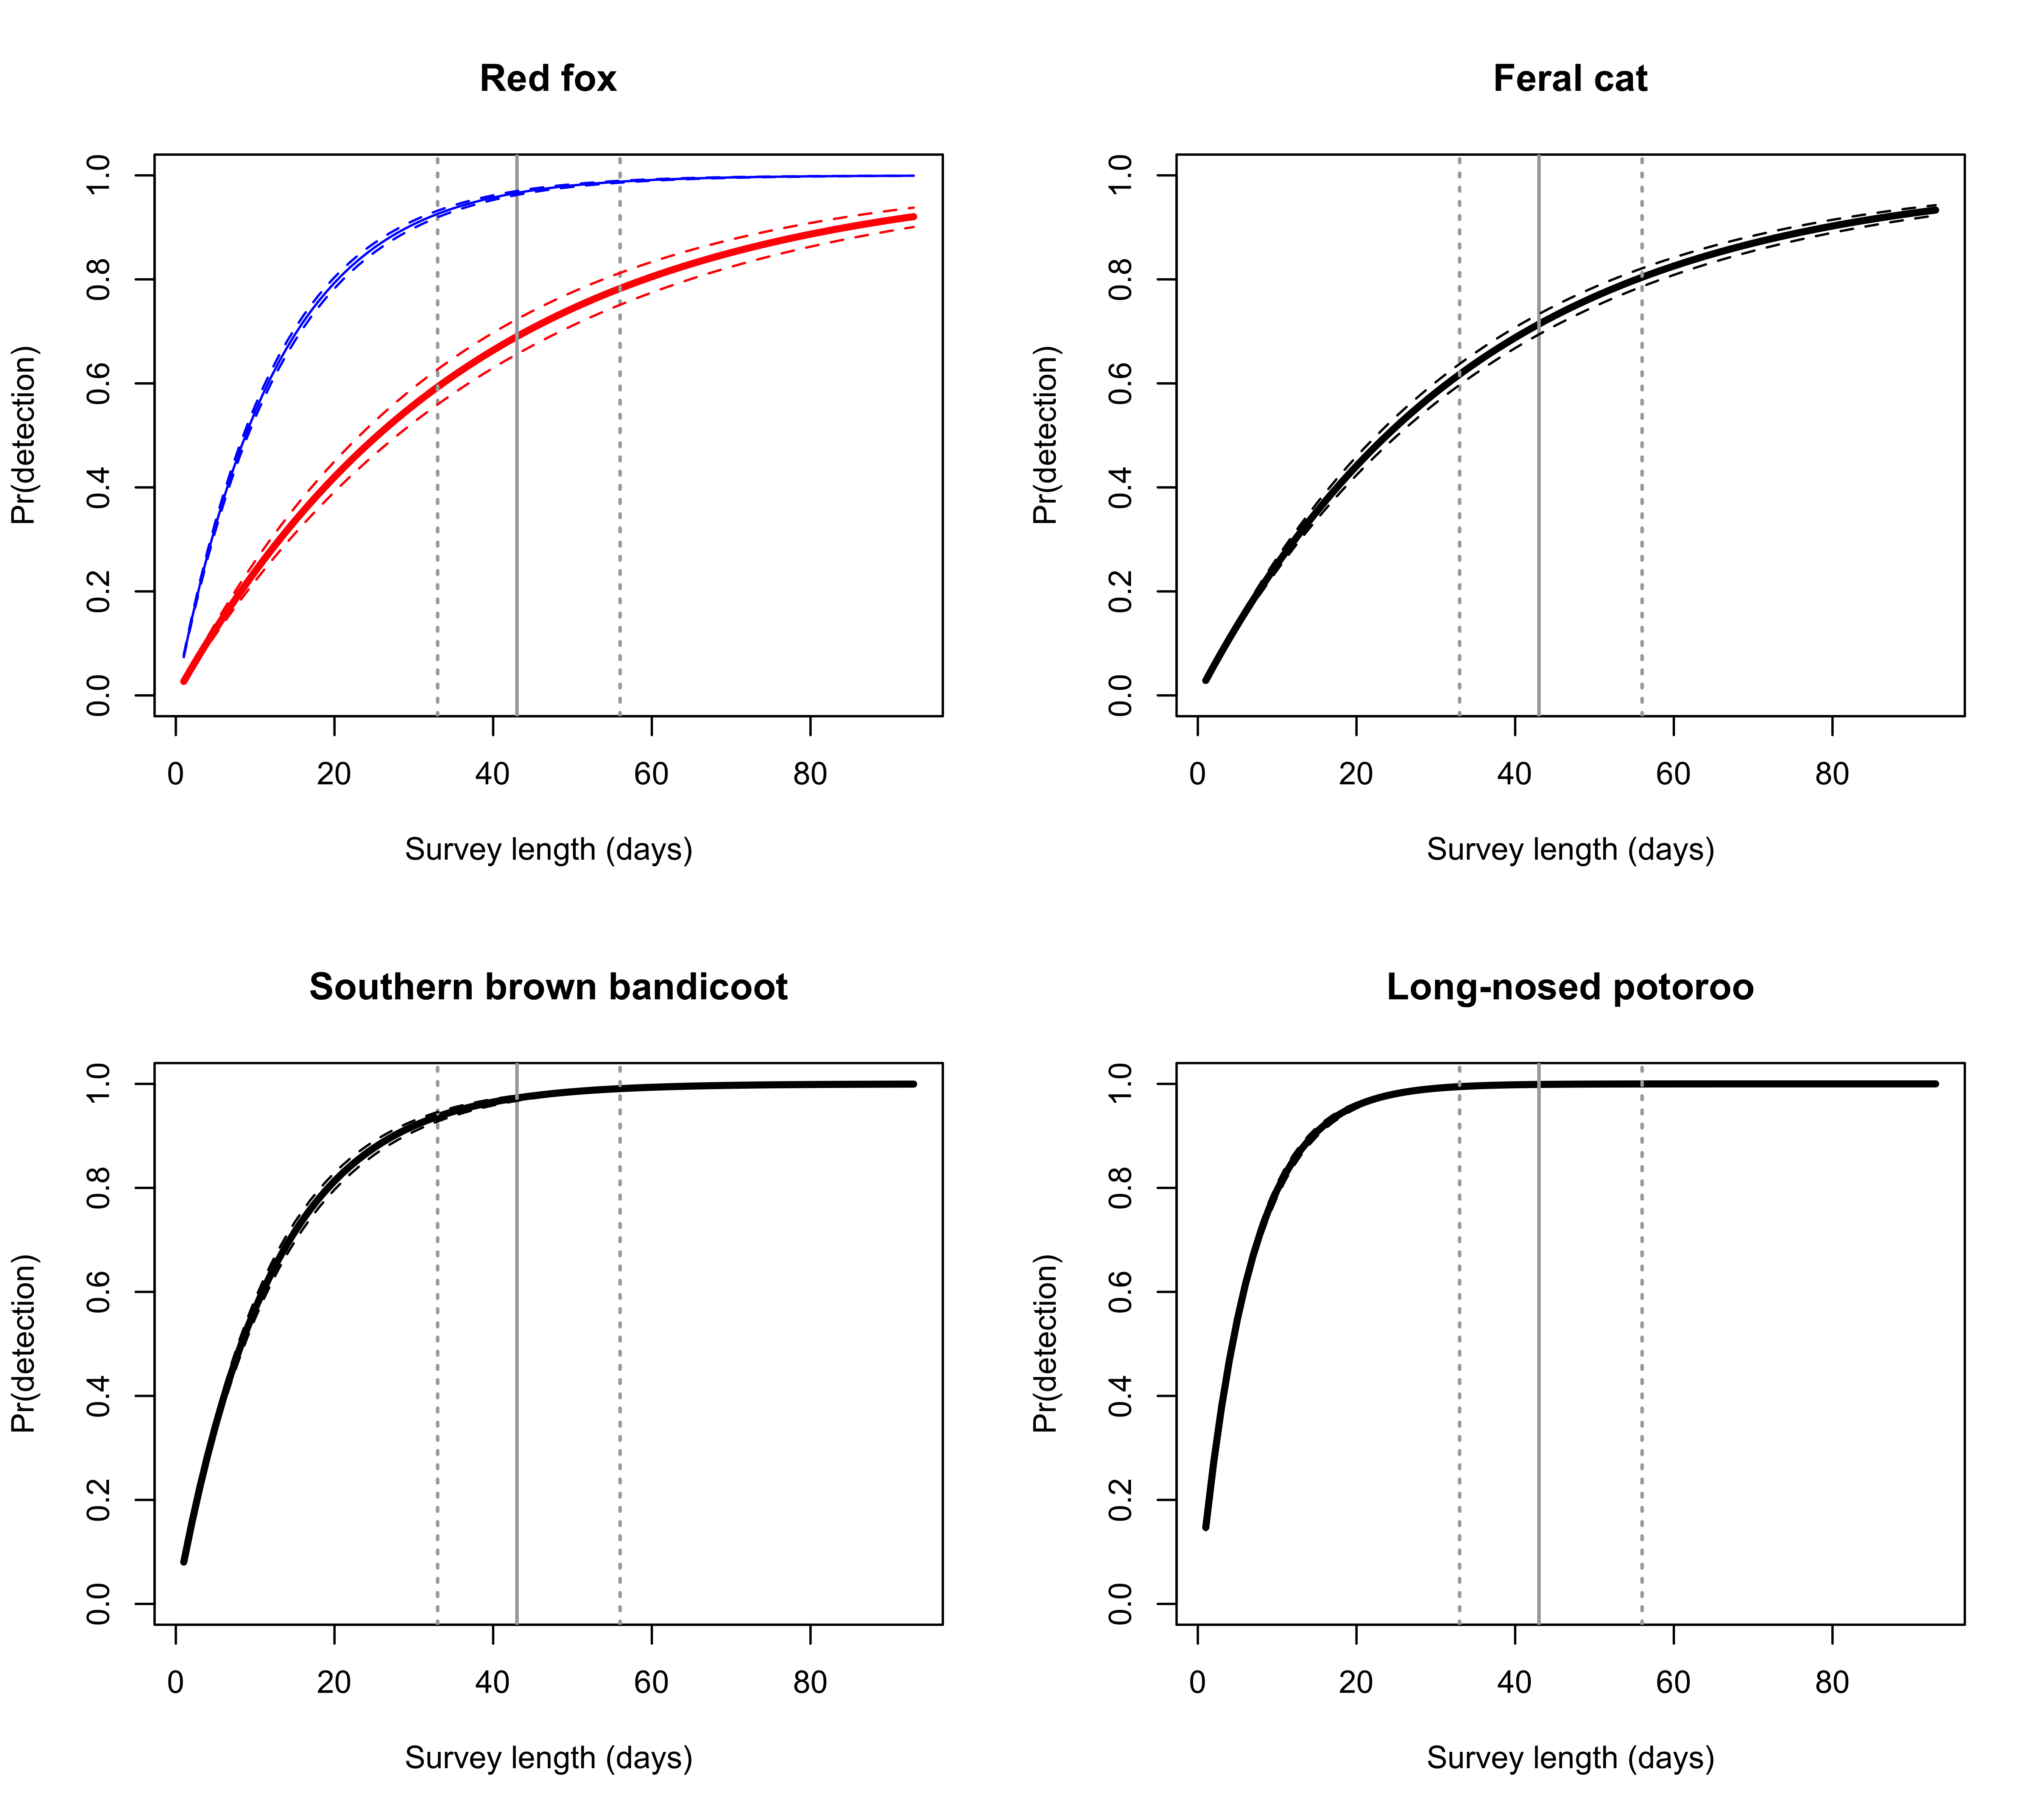
\includegraphics[width=1\linewidth]{figure/c1/detectability} 

}

\caption{Cumulative detection probability for surveyed species averaged across all sites (solid black lines), as well as sites with fox control (solid red line) and without fox control (solid blue line). Dashed lines represent 95\% confidence intervals. Vertical grey lines represent mean (solid) as well as 25\% and 75\% quantiles (dotted) of days camera-traps were active for.}\label{fig:occ-cumdet}
\end{figure}
\newpage

\(~\)

\(~\)

\(~\)
\begin{figure}

{\centering 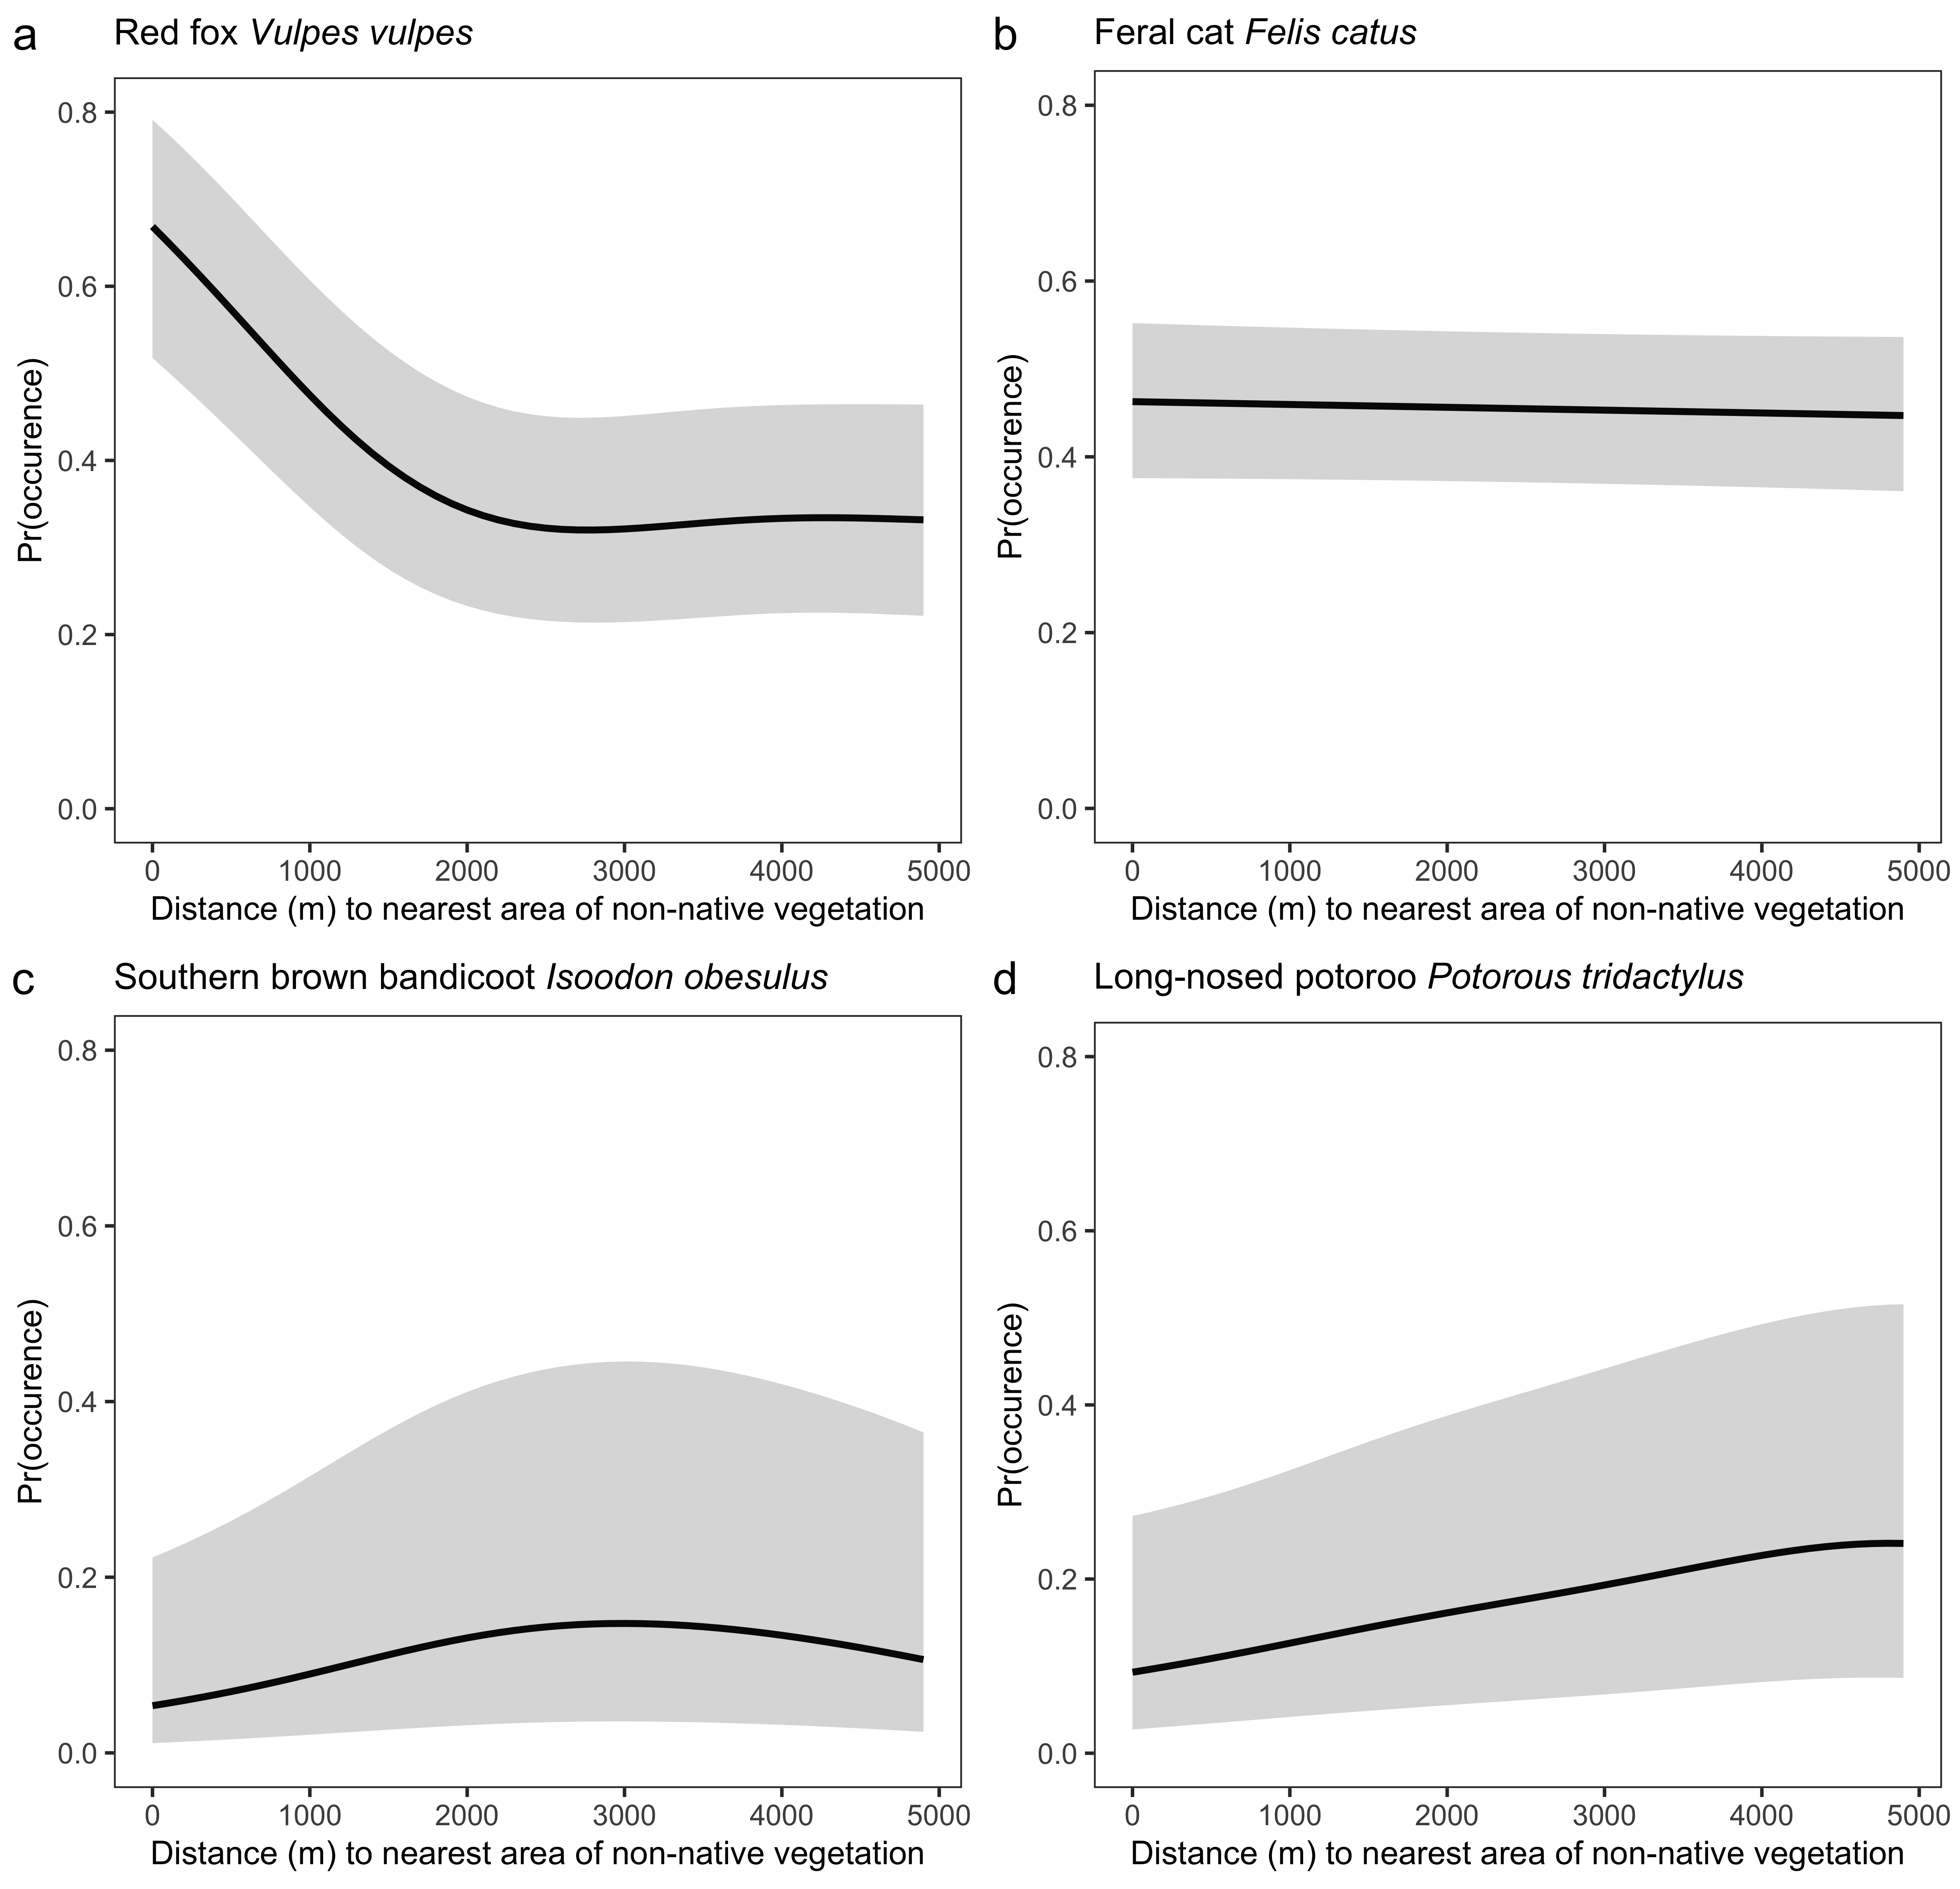
\includegraphics[width=1\linewidth]{figure/c1/dist_edge} 

}

\caption{Fox occurrence probability decreased linearly for 2 km as distance to the nearest area of non-native vegetation (larger than 30 ha) increased (a). Increasing distance to non-native vegetation had a weak, positive effect on long-nosed potoroo's (d), but little-no impact on feral cats (b) and southern brown bandicooots (c) in south-west Victoria, Australia. Shaded regions indicate 95\% confidence intervals.}\label{fig:occ-dist}
\end{figure}
\newpage

\hypertarget{otways17-app}{%
\chapter{Supporting Information: Chapter \ref{otways17}}\label{otways17-app}}

\newpage

\(~\)

\(~\)

\(~\)
\begin{figure}

{\centering 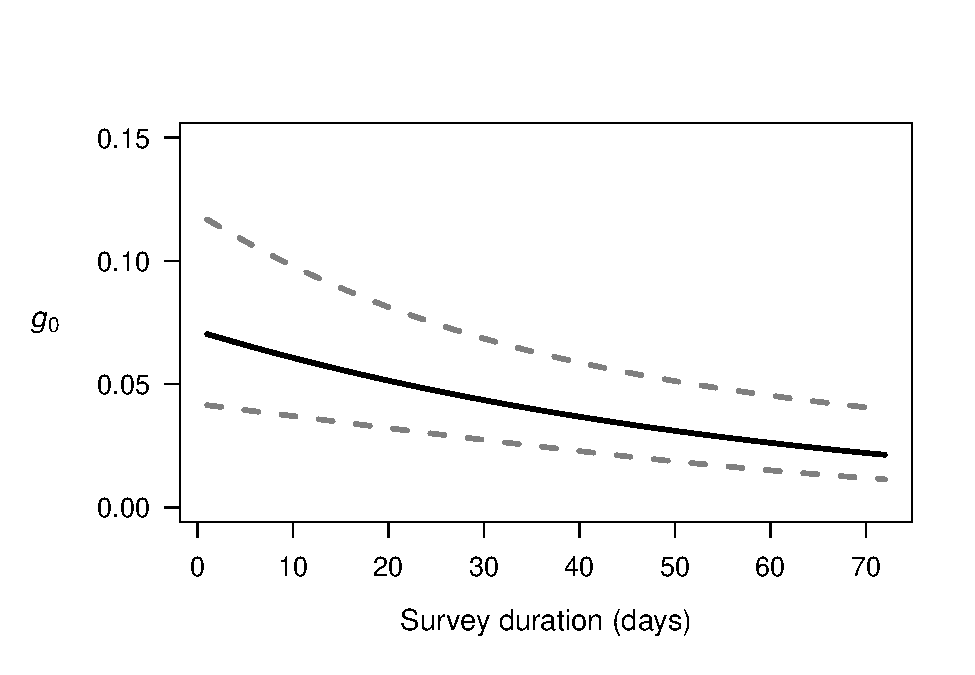
\includegraphics[width=0.7\linewidth]{figure/otways17-g0t-1} 

}

\caption{The AICc-best model linear trend in \textit{g}0 values (probability of daily detection in activity centre) throughout the survey. Grey dashed lines indicate 95\% confidence intervals.}\label{fig:otways17-g0t}
\end{figure}
\newpage

\(~\)

\(~\)

\(~\)

\begingroup\fontsize{10}{12}\selectfont
\begin{longtable}[t]{lrrrrrrr}
\caption{\label{tab:otways17-detfn}Model selection table and density estimates for different detection function shapes for spatial mark-resight models.}\\
\toprule
\multicolumn{5}{c}{Model comparison} & \multicolumn{3}{c}{Density estimate (cats km-2)} \\
\cmidrule(l{3pt}r{3pt}){1-5} \cmidrule(l{3pt}r{3pt}){6-8}
Detector function & K & AICc & dAICc & AICcwt & estimate & lcl & ucl\\
\midrule
\endfirsthead
\caption[]{\label{tab:otways17-detfn}Model selection table and density estimates for different detection function shapes for spatial mark-resight models. \textit{(continued)}}\\
\toprule
\multicolumn{5}{c}{Model comparison} & \multicolumn{3}{c}{Density estimate (cats km-2)} \\
\cmidrule(l{3pt}r{3pt}){1-5} \cmidrule(l{3pt}r{3pt}){6-8}
Detector function & K & AICc & dAICc & AICcwt & estimate & lcl & ucl\\
\midrule
\endhead

\endfoot
\bottomrule
\multicolumn{8}{l}{\rule{0pt}{1em}K - number of parameters}\\
\multicolumn{8}{l}{\rule{0pt}{1em}AICc - Akaike's Information Criterion with small-sample adjustment}\\
\multicolumn{8}{l}{\rule{0pt}{1em}dAICc - difference between AICc of this model and the model with smallest AICc}\\
\multicolumn{8}{l}{\rule{0pt}{1em}AICcwt - AICc model weight}\\
\multicolumn{8}{l}{\rule{0pt}{1em}lcl – lower 95\% confidence limit}\\
\multicolumn{8}{l}{\rule{0pt}{1em}ucl – upper 95\% confidence limit}\\
\endlastfoot
hazard-rate & 4 & 2359.59 & 0.00 & 0.7 & 1.15 & 0.93 & 1.42\\
exponential & 3 & 2361.25 & 1.66 & 0.3 & 1.19 & 0.96 & 1.49\\
halfnormal & 3 & 2373.30 & 13.72 & 0.0 & 1.12 & 0.93 & 1.35\\*
\end{longtable}
\endgroup{}

\hypertarget{density-app}{%
\chapter{Supporting Information: Chapter \ref{density}}\label{density-app}}

\newpage

\hypertarget{density-app-field}{%
\section{Field surveys}\label{density-app-field}}

In the Glenelg region, we deployed camera-traps once at a unique sites once. In the Otway region, we redeployed camera-traps in sites three times annually. All 2017 camera-sites were resurveyed each year, except for four logistically challenging sites in the southern grid. In 2018, we added 16 additional sites in the southern grid, as well as 36 additional sites in the northern grid. These additional sites were resurveyed in 2019.

At each site, we deployed a singular remote trail camera with infrared flash and temperature-in-motion detector. The vast majority of camera-traps were Reconyx Hyperfire HC600, but a small portion was made up of both PC900 and HF2X infrared models (Reconyx, Holmen, Wisconsin). We programmed camera's to the highest sensitivity and to take five consecutive photographs when triggered (no quiet period). We attached each camera to a tree, approximately 30 cm above the ground, and facing toward a lure 2 - 2.5 metres away. The lure comprised an oil-absorbing cloth doused in tuna oil and placed inside a PVC pipe container with a mesh top. We secured each lure to the top of a 1 metre wooden stake and attached a handful of small white feathers to the outside of the PVC pipe container. Feathers were not used in the Lower Glenelg National Park survey. We cleared vegetation in the camera's line-of-sight to reduce false triggers and avoid obscuring cat coat markings in images.

\newpage

\(~\)

\(~\)

\(~\)
\begin{figure}

{\centering 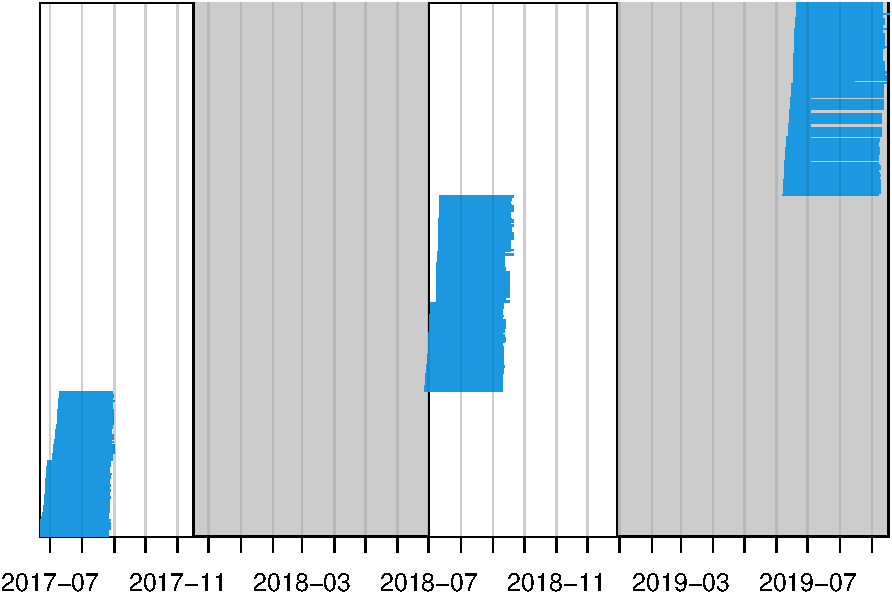
\includegraphics[width=1\linewidth]{figure/density-camop-1} 

}

\caption{Camera-trap operation times in the Otway region, Australia. Each blue horizontal line represents one camera-trap deployment. Grey shading indicates periods of fox control in the impact landscape.}\label{fig:density-camop}
\end{figure}
\newpage

\(~\)

\(~\)

\(~\)
\begin{figure}

{\centering 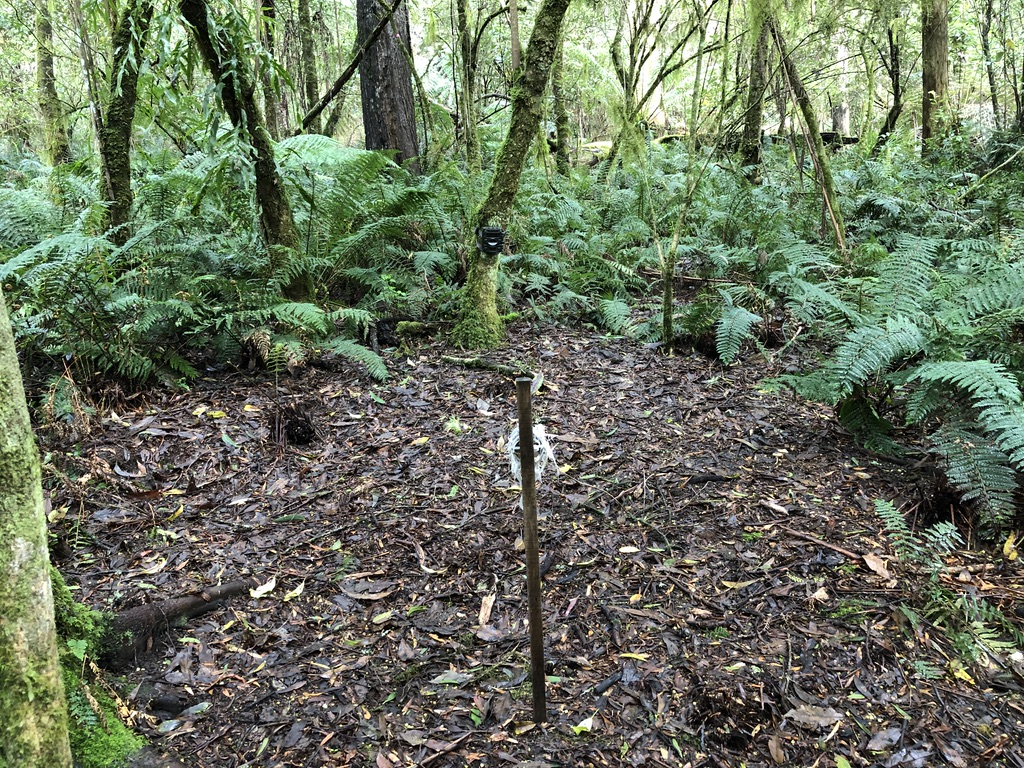
\includegraphics[width=1\linewidth]{figure/c3/camtrap1} 

}

\caption{Example of a typical camera-trap set-up in the Otway region, Australia.}\label{fig:density-cam-photo}
\end{figure}
\newpage

\hypertarget{density-app-id}{%
\section{Individual cat identification}\label{density-app-id}}

We first labelled every camera-trap image with a species metadata tag using \href{https://www.digikam.org}{DigiKam software}. We also added metadata tags for each cat coat type: black, mackerel tabby, classic tabby, ginger and other (coats with multiple colour blends; Fig. 3). This allowed us to summarise species records and extract cat images using the `camtrapR' R-package (Niedballa \emph{et al.} 2016).

We considered all black cats to be of the `unmarked' category in spatial mark-resight models - even the few with white splotches on their underside (as these couldn't always be seen as cats move with their head down).

In the remaining coat categories where possible, we identified individual cats based on their unique coat markings. The ability to identify individuals substantially increased as the image library for each cat increased. Therefore we made the easiest identifications first to build up these libraries, before making decisions on the less obvious detections. We examined and matched all coat markings seen between two particular defections. Markings on the front legs were the most useful for ID's as the patterns do not skew as much with different body positions. On the whole, unidentifiable detections were mainly due to only part of a cat appearing in the frame, or because photos were blurry (because of cat movement or a foggy camera lens).

We were left with a small number of instances (less than ten) where only left or right flanks could be seen. In this case, the side with the most repeat detections was labelled as an individual, whereas the side with the least number of detections was considered unidentifiable. Additionally, an extremely small portion of cats in the Otways had ginger coats. When ginger coats are photographed with an infrared flash, they become overexposed and no markings can be seen (see the image in bottom-right corner in Fig. S3). We only had one detection of a ginger cat without an infrared coat. Therefore, if there were multiple ginger cat detections in a single grid, we treated them in the same way as one-sided flank detections.

One observer identified the 2018 feral cats in the Glenelg region (MR) and the 2021 Lower Glenelg National Park cats (Luke Woodford). In the 2017 and 2018 Otway datasets (where there were substantially more cat detections and fewer distinct coat patterns) two independent observers identified individual cats and discrepancies between observers were reviewed together until consensus was reached (MR, MLP, BH). If no consensus was reached, the cat was considered unidentifiable. In the 2019 Otway dataset, many of the identified cats were sighted in the previous surveys -- these larger individual libraries meant that cats could be identified more easily so only one observer was necessary (MR). We also made use of additional cat images taken within the Otway region grids (just before each of our surveys) by white flash camera-traps from another study (Zoï Banikos, unpublished data). This provided additional and higher quality images (due to the white flash) of individuals in the photo library for identifications.

We were therefore left with three groups of cats: unmarked (black cats), marked (cats which could be identified to the individual-level with complete certainty) and mark status unknown (cats which were not black, but couldn't be identified to the individual level with complete certainty).

We ignored the few detections of cats which were obviously young enough to be dependent on a parent, as these kittens do not have independent activity centres or movements and were not yet recruited into the adult population.

\newpage

\(~\)

\(~\)

\(~\)
\begin{figure}

{\centering 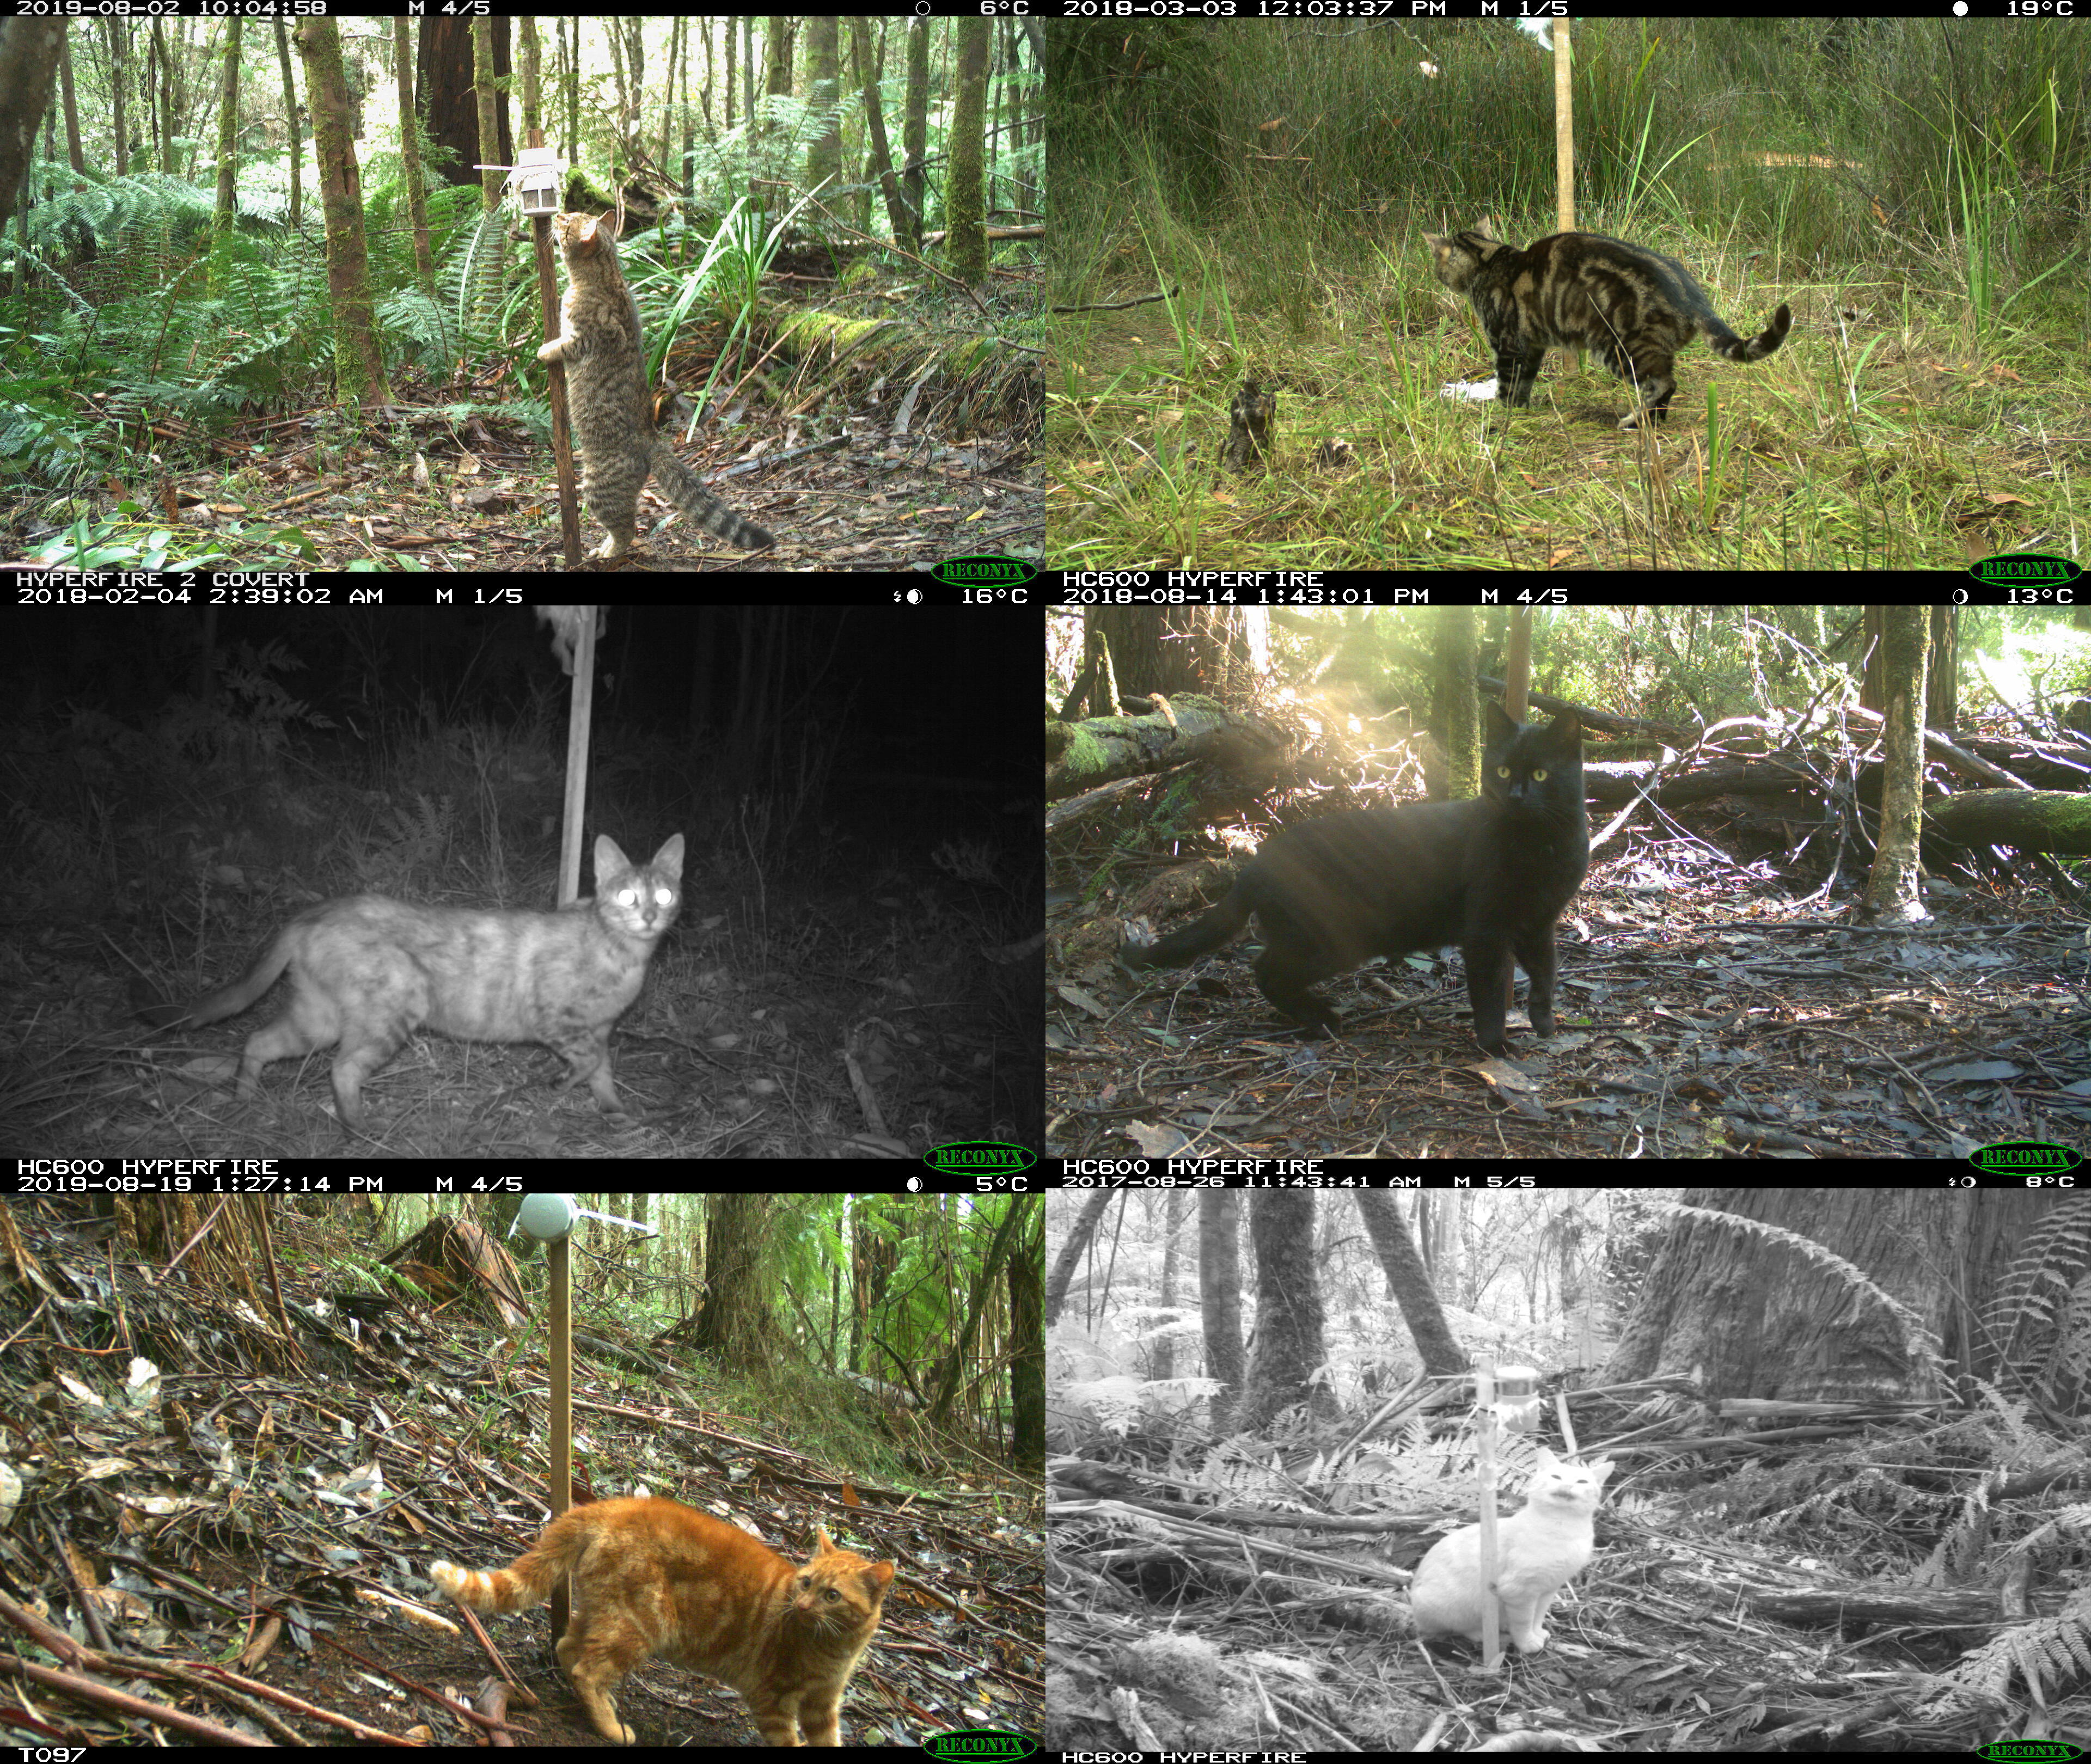
\includegraphics[width=1\linewidth]{figure/c3/cat_coats} 

}

\caption{Feral cat coat categories from left-right, top-bottom: black, mackerel tabby, classic tabby, other, black, ginger and ginger with infrared flash.}\label{fig:density-cat-photo}
\end{figure}
\newpage

\hypertarget{summary-statistics}{%
\section{Summary statistics}\label{summary-statistics}}

\(~\)

\(~\)

\(~\)

\begingroup\fontsize{10}{12}\selectfont
\begin{longtable}[t]{lrrrrrrr}
\caption{\label{tab:density-stats}Summary of camera-trap survey effort and feral cat detections.}\\
\toprule
\multicolumn{5}{c}{ } & \multicolumn{3}{c}{Detections (max. 1 per 24-hr)} \\
\cmidrule(l{3pt}r{3pt}){6-8}
Landscape & Cameras & Trapnights & Cats & Moves & Identified & Unidentified & Unmarked\\
\midrule
\endfirsthead
\caption[]{\label{tab:density-stats}Summary of camera-trap survey effort and feral cat detections. \textit{(continued)}}\\
\toprule
\multicolumn{5}{c}{ } & \multicolumn{3}{c}{Detections (max. 1 per 24-hr)} \\
\cmidrule(l{3pt}r{3pt}){6-8}
Landscape & Cameras & Trapnights & Cats & Moves & Identified & Unidentified & Unmarked\\
\midrule
\endhead

\endfoot
\bottomrule
\endlastfoot
Annya & 110 & 8000 & 9 & 11 & 23 & 3 & 20\\
Cobbob & 110 & 7752 & 13 & 19 & 35 & 9 & 37\\
Hotspur & 99 & 6085 & 8 & 12 & 22 & 3 & 13\\
Mt Clay & 106 & 5451 & 10 & 16 & 33 & 5 & 0\\
LGNP north & 49 & 2102 & 6 & 3 & 11 & 0 & 0\\
\addlinespace
LGNP south & 64 & 2842 & 21 & 4 & 37 & 0 & 0\\
North 2017 & 67 & 3565 & 26 & 12 & 60 & 8 & 46\\
South 2017 & 73 & 7099 & 20 & 18 & 62 & 4 & 48\\
North 2018 & 103 & 7838 & 30 & 32 & 90 & 12 & 62\\
South 2018 & 85 & 4543 & 24 & 37 & 75 & 17 & 59\\
\addlinespace
North 2019 & 99 & 6077 & 27 & 39 & 90 & 22 & 101\\
South 2019 & 86 & 7150 & 25 & 69 & 133 & 23 & 58\\*
\end{longtable}
\endgroup{}

\newpage

\hypertarget{feral-cat-detection-plots}{%
\section{Feral cat detection plots}\label{feral-cat-detection-plots}}

\hypertarget{glenelg-region}{%
\subsection{Glenelg region}\label{glenelg-region}}

\hypertarget{replicate-1}{%
\subsubsection{Replicate 1}\label{replicate-1}}

\(~\)

\(~\)

\(~\)
\begin{figure}

{\centering 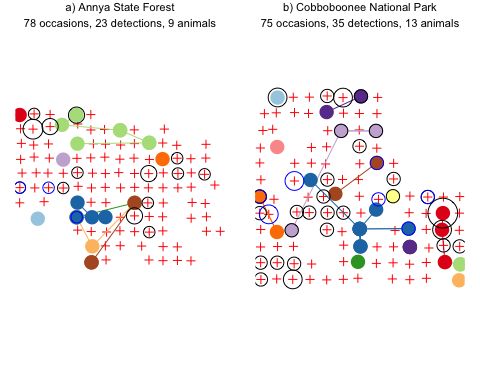
\includegraphics[width=1\linewidth]{figure/density-plot-ch-1-1} 

}

\caption{Feral cat detections in the first replicate grid pair in the Glenelg region, Australia. Camera-traps are indicated by red crosses. Solid fill coloured circles represent identified cats with lines indicating observed movements. Black open circles indicate black cat detections; blue circles indicate unidentifiable tabby cat detections, with circle radius scaling positively with the number of daily detections. Fox control does not occur in Annya (a) but does in Cobboboonee (b).}\label{fig:density-plot-ch-1}
\end{figure}
\newpage

\hypertarget{replicate-2}{%
\subsubsection{Replicate 2}\label{replicate-2}}

\(~\)

\(~\)

\(~\)
\begin{figure}

{\centering 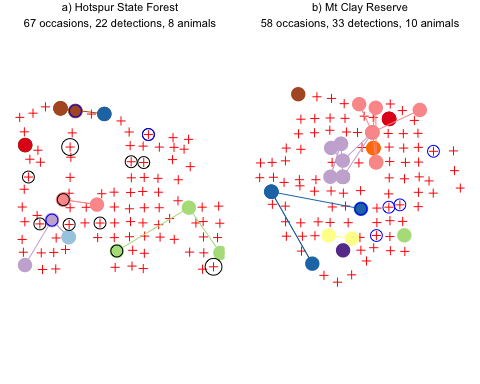
\includegraphics[width=1\linewidth]{figure/density-plot-ch-2-1} 

}

\caption{Feral cat detections in the second replicate grid pair in the Glenelg region, Australia. Camera-traps are indicated by red crosses. Solid fill coloured circles represent identified cats with lines indicating observed movements. Black open circles indicate black cat detections; blue circles indicate unidentifiable tabby cat detections, with circle radius scaling positively with the number of daily detections. Fox control does not occur in Hotspur (a) but does in Mt Clay (b).}\label{fig:density-plot-ch-2}
\end{figure}
\newpage

\hypertarget{replicate-3}{%
\subsubsection{Replicate 3}\label{replicate-3}}

\(~\)

\(~\)

\(~\)
\begin{figure}

{\centering 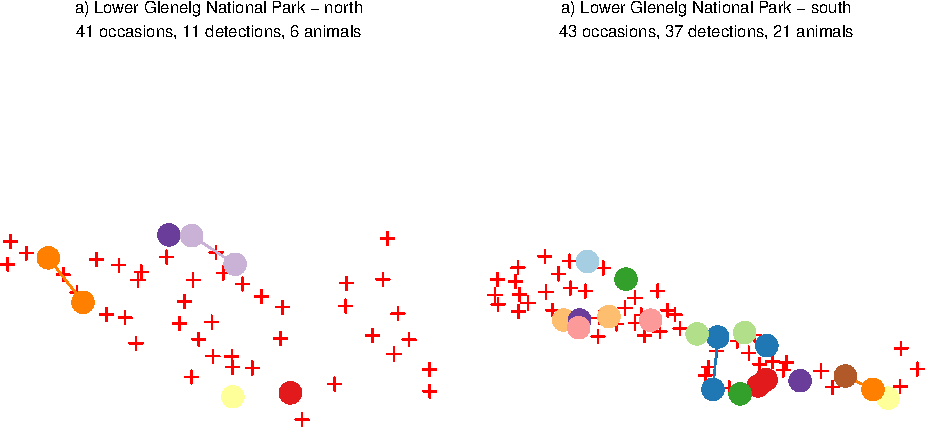
\includegraphics[width=1\linewidth]{figure/density-plot-ch-3-1} 

}

\caption{Feral cat detections in the third replicate grid pair in the Glenelg region, Australia. Camera-traps are indicated by red crosses. Solid fill coloured circles represent identified cats with lines indicating observed movements. Black open circles indicate black cat detections; blue circles indicate unidentifiable tabby cat detections, with circle radius scaling positively with the number of daily detections. Fox control does not occur in the north (a) but does in the south (b).}\label{fig:density-plot-ch-3}
\end{figure}
\newpage

\hypertarget{otway-region}{%
\subsection{Otway region}\label{otway-region}}

\hypertarget{section}{%
\subsubsection{2017}\label{section}}

\(~\)

\(~\)

\(~\)
\begin{figure}

{\centering 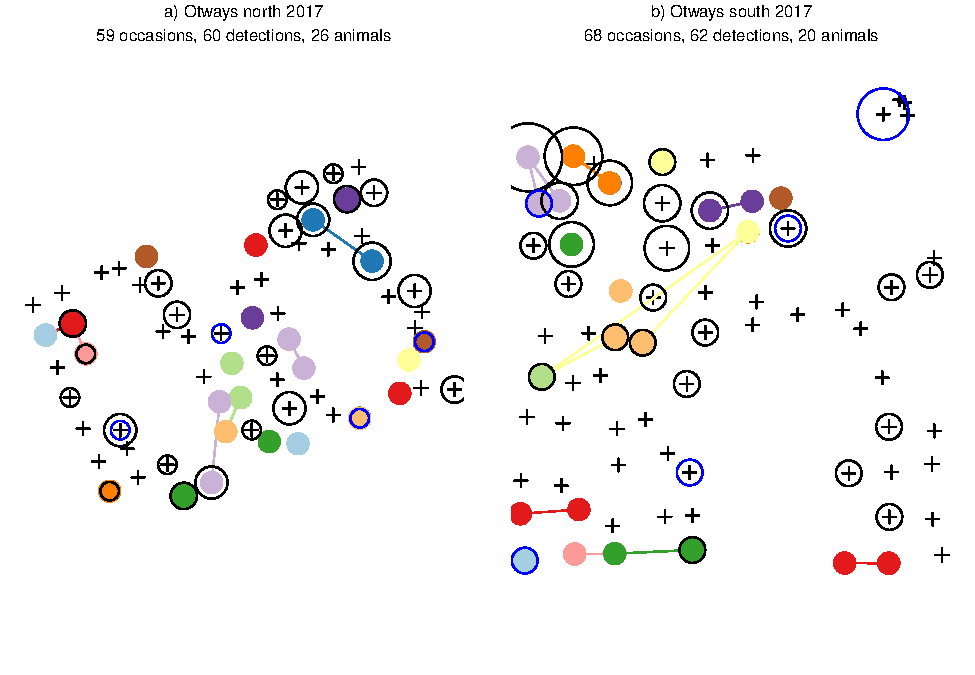
\includegraphics[width=1\linewidth]{figure/density-plot-ch-4-1} 

}

\caption{Feral cat detections in the Otway region, Australia, 2017. Solid fill coloured circles represent identified cats with lines indicating observed movements. Black open circles indicate black cat detections; blue circles indicate unidentifiable tabby cat detections, with circle radius scaling positively with the number of daily detections. Fox control did not occur in either of the landscapes during this time.}\label{fig:density-plot-ch-4}
\end{figure}
\newpage

\hypertarget{section-1}{%
\subsubsection{2018}\label{section-1}}

\(~\)

\(~\)

\(~\)
\begin{figure}

{\centering 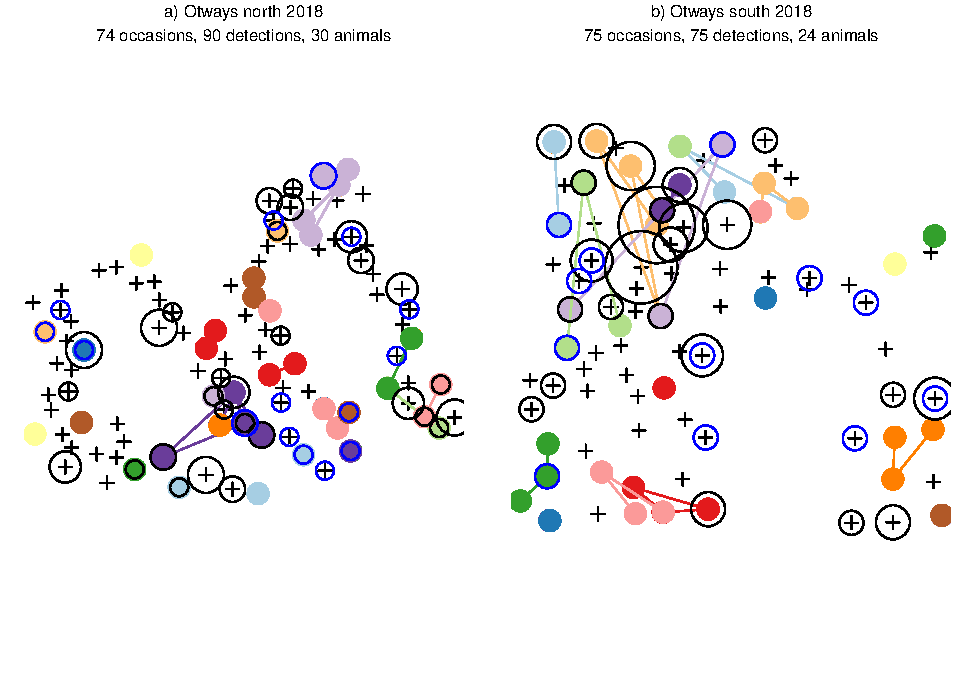
\includegraphics[width=1\linewidth]{figure/density-plot-ch-5-1} 

}

\caption{Feral cat detections in the Otway region, Australia, 2018. Solid fill coloured circles represent identified cats with lines indicating observed movements. Black open circles indicate black cat detections; blue circles indicate unidentifiable tabby cat detections, with circle radius scaling positively with the number of daily detections. Fox control had occurred, but lapsed just prior to the survey in the northern landscape (a), and did not occur in the southern landscape (b).}\label{fig:density-plot-ch-5}
\end{figure}
\newpage

\hypertarget{section-2}{%
\subsubsection{2019}\label{section-2}}

\(~\)

\(~\)

\(~\)
\begin{figure}

{\centering 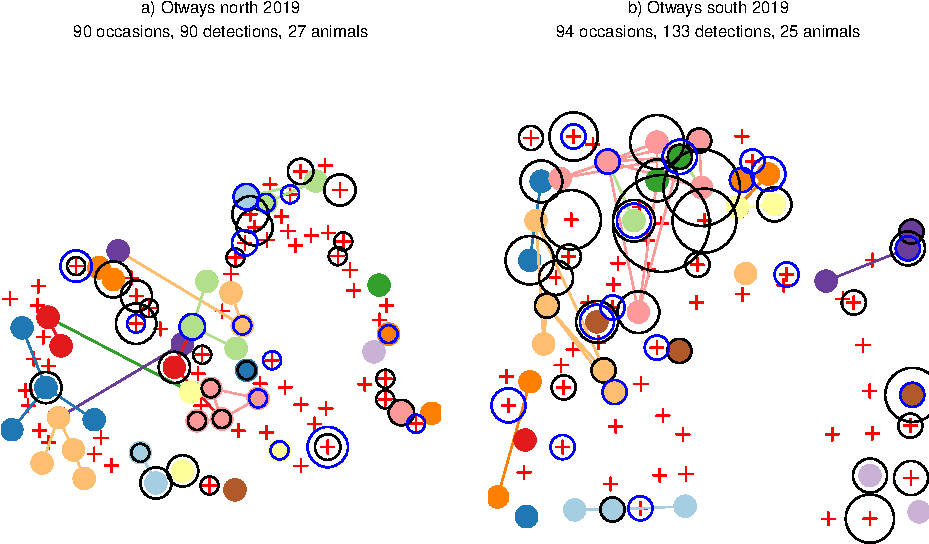
\includegraphics[width=1\linewidth]{figure/density-plot-ch-6-1} 

}

\caption{Feral cat detections in the Otway region, Australia, 2019. Solid fill coloured circles represent identified cats with lines indicating observed movements. Black open circles indicate black cat detections; blue circles indicate unidentifiable tabby cat detections, with circle radius scaling positively with the number of daily detections. Fox control occurred in the northern landscape (a) during this survey, but not the southern landscape (b).}\label{fig:density-plot-ch-6}
\end{figure}
\newpage

\hypertarget{density-app-fox}{%
\section{Fox spatial occurrence}\label{density-app-fox}}

\hypertarget{glenelg-region-1}{%
\subsection{Glenelg region}\label{glenelg-region-1}}

\(~\)

\(~\)

\(~\)
\begin{verbatim}

Family: binomial 
Link function: logit 

Formula:
fox ~ s(x, y, bs = "ds", m = c(1, 0.5), k = 200) + offset(log(survey_duration))

Parametric coefficients:
            Estimate Std. Error z value Pr(>|z|)    
(Intercept) -4.53965    0.09293  -48.85   <2e-16 ***
---
Signif. codes:  0 '***' 0.001 '**' 0.01 '*' 0.05 '.' 0.1 ' ' 1

Approximate significance of smooth terms:
         edf Ref.df Chi.sq  p-value    
s(x,y) 25.58    199  61.78 9.75e-07 ***
---
Signif. codes:  0 '***' 0.001 '**' 0.01 '*' 0.05 '.' 0.1 ' ' 1

R-sq.(adj) =  0.126   Deviance explained = 13.1%
fREML = 845.52  Scale est. = 1         n = 538
\end{verbatim}
\newpage

\(~\)

\(~\)

\(~\)
\begin{figure}

{\centering 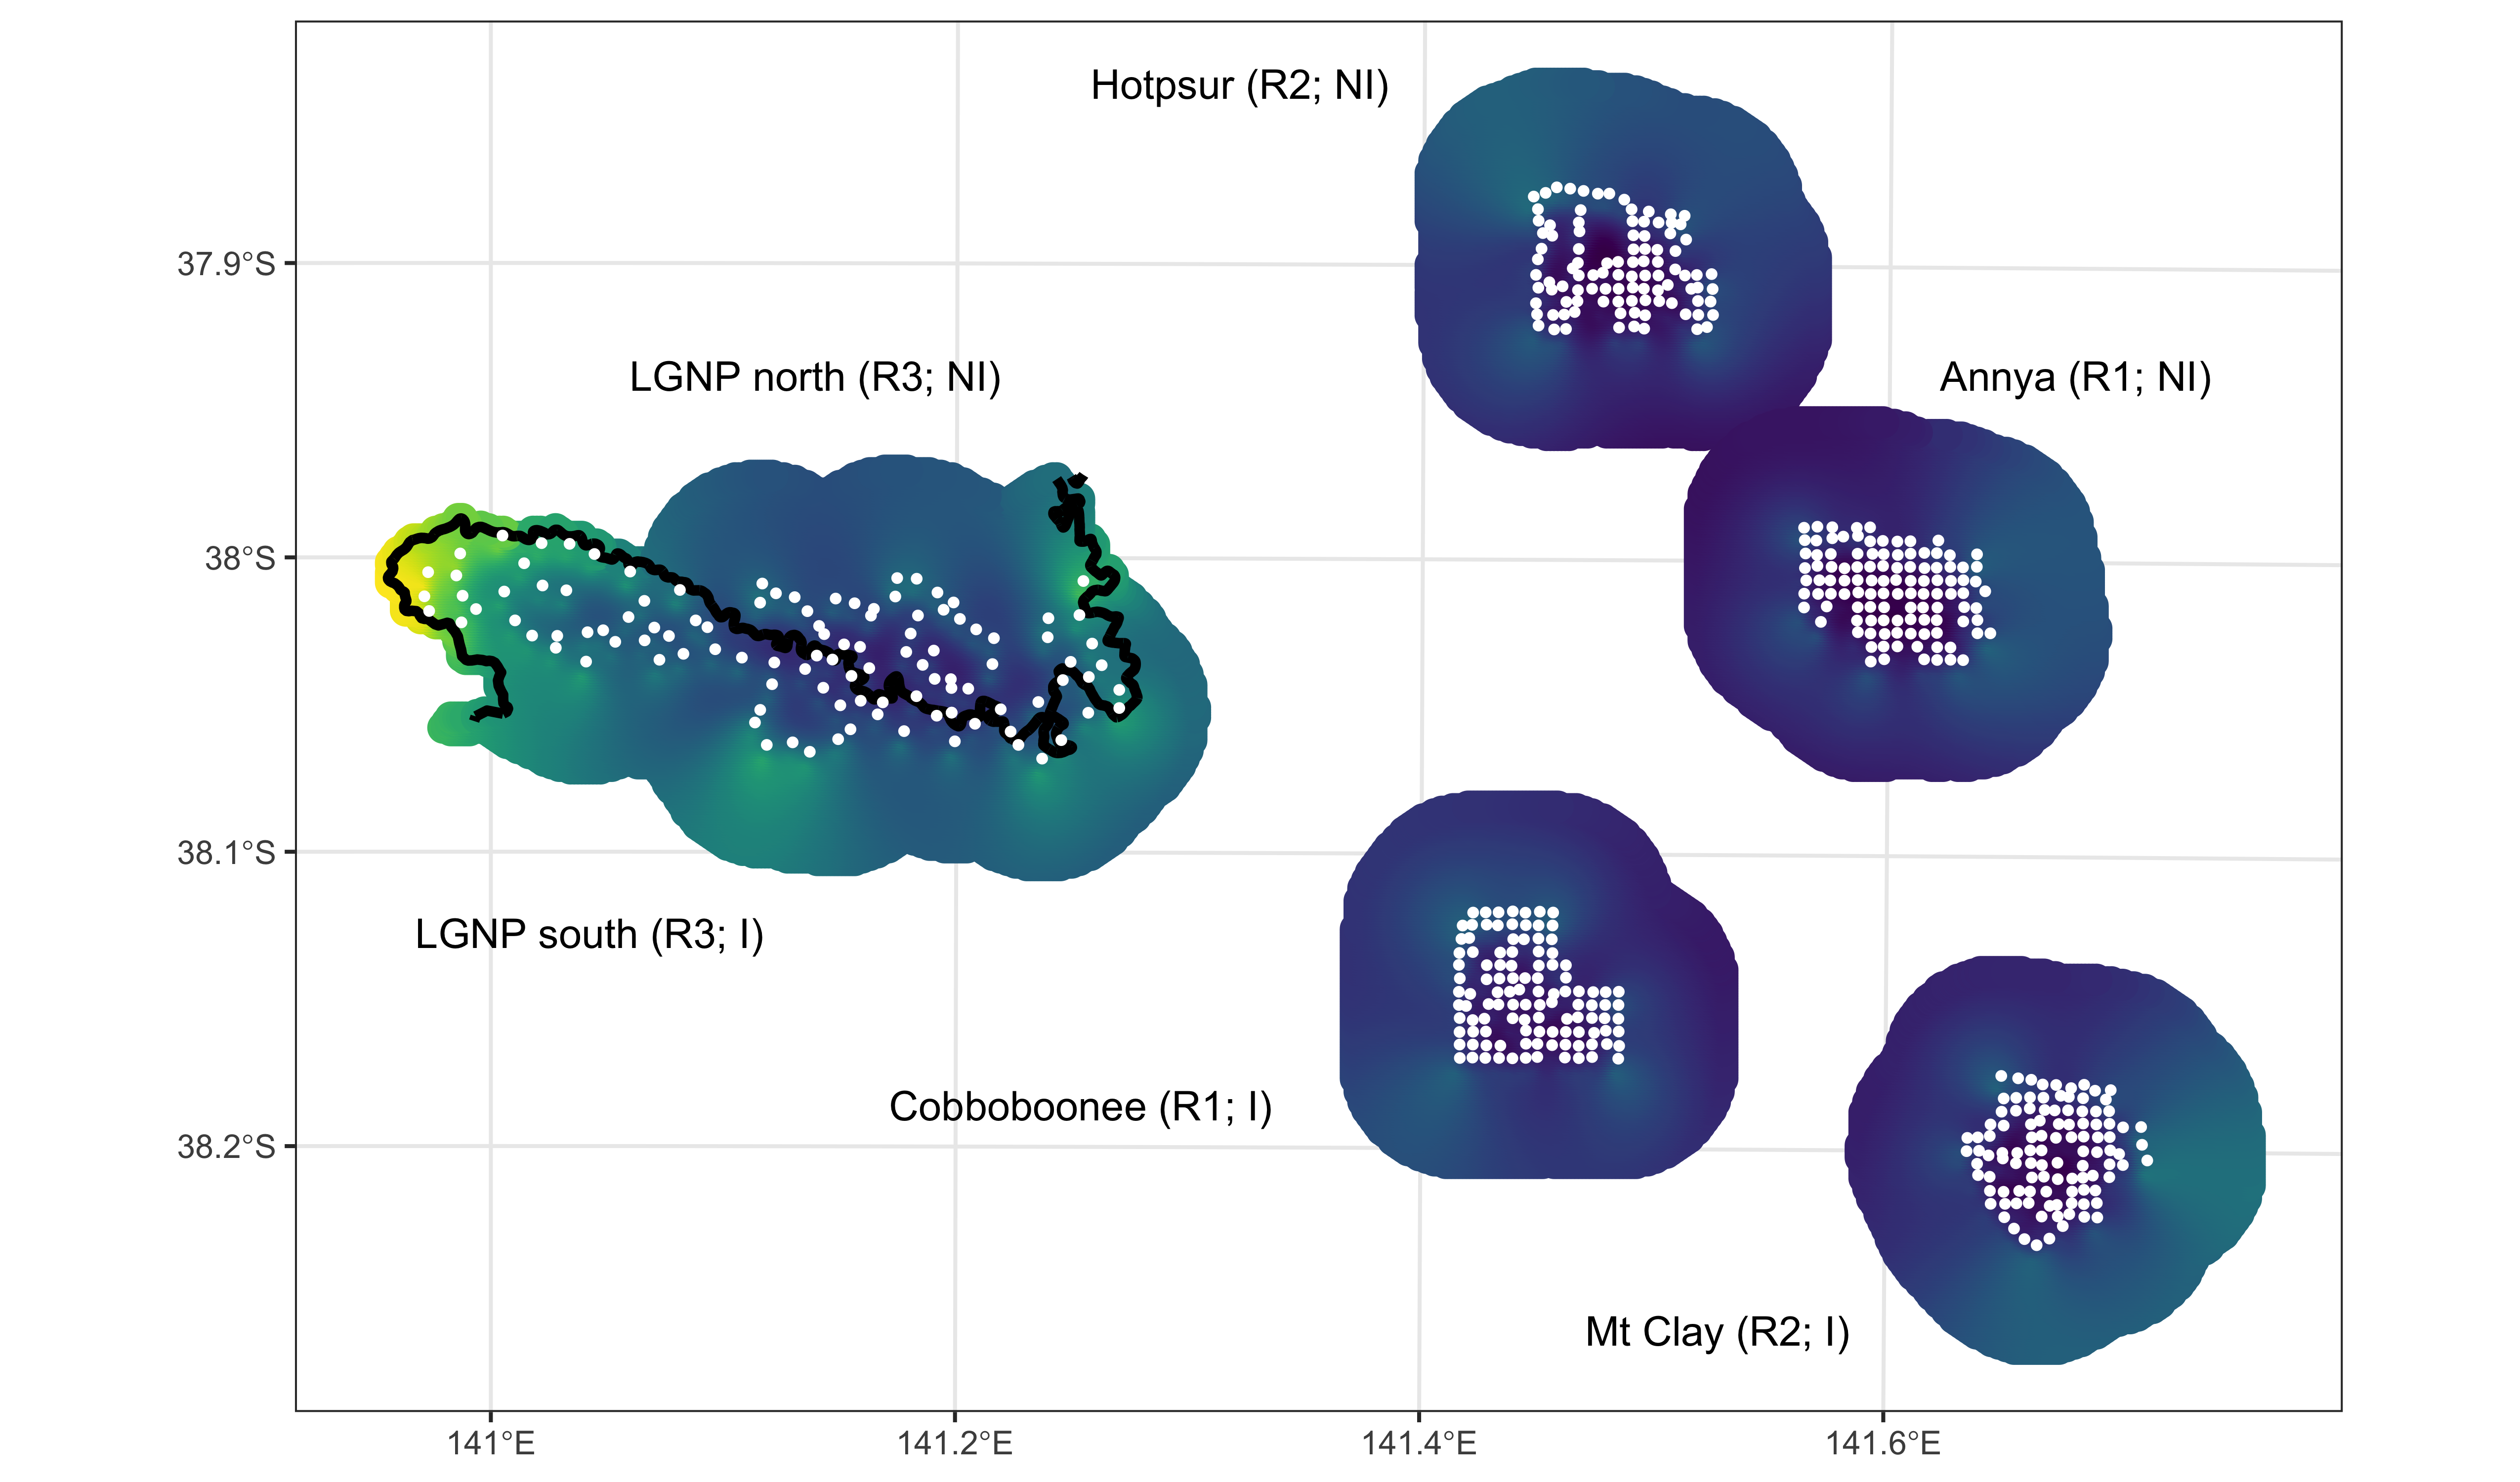
\includegraphics[width=1\linewidth]{figure/c3/fox_occ_se_glenelg_600dpi} 

}

\caption{Standard error estimate of log fox occurrence probability derived from generalised additive models within each impact (I) and associated non-impact (NI) landscape in the Glenelg region, Australia.}\label{fig:density-fox-se-g}
\end{figure}
\newpage

\hypertarget{otway-region-1}{%
\subsection{Otway Region}\label{otway-region-1}}

\(~\)

\(~\)

\(~\)
\begin{verbatim}

Family: binomial 
Link function: logit 

Formula:
fox ~ year + s(x, y, by = year, bs = "ds", m = c(1, 0.5), k = 100) + 
    s(station, bs = "re") + offset(log(survey_duration))

Parametric coefficients:
             Estimate Std. Error z value Pr(>|z|)    
(Intercept) -5.283154   0.230023 -22.968   <2e-16 ***
year2018     0.004643   0.277696   0.017    0.987    
year2019     0.037119   0.282270   0.132    0.895    
---
Signif. codes:  0 '***' 0.001 '**' 0.01 '*' 0.05 '.' 0.1 ' ' 1

Approximate significance of smooth terms:
                      edf Ref.df Chi.sq  p-value    
s(x,y):year2017 2.688e+00     99  8.096 0.010597 *  
s(x,y):year2018 2.494e-05     99  0.000 0.506341    
s(x,y):year2019 6.148e+00     99 22.262 0.000380 ***
s(station)      5.366e+01    194 75.723 0.000116 ***
---
Signif. codes:  0 '***' 0.001 '**' 0.01 '*' 0.05 '.' 0.1 ' ' 1

R-sq.(adj) =   0.24   Deviance explained = 27.8%
fREML = 763.36  Scale est. = 1         n = 513
\end{verbatim}
\newpage

\(~\)

\(~\)

\(~\)
\begin{figure}

{\centering 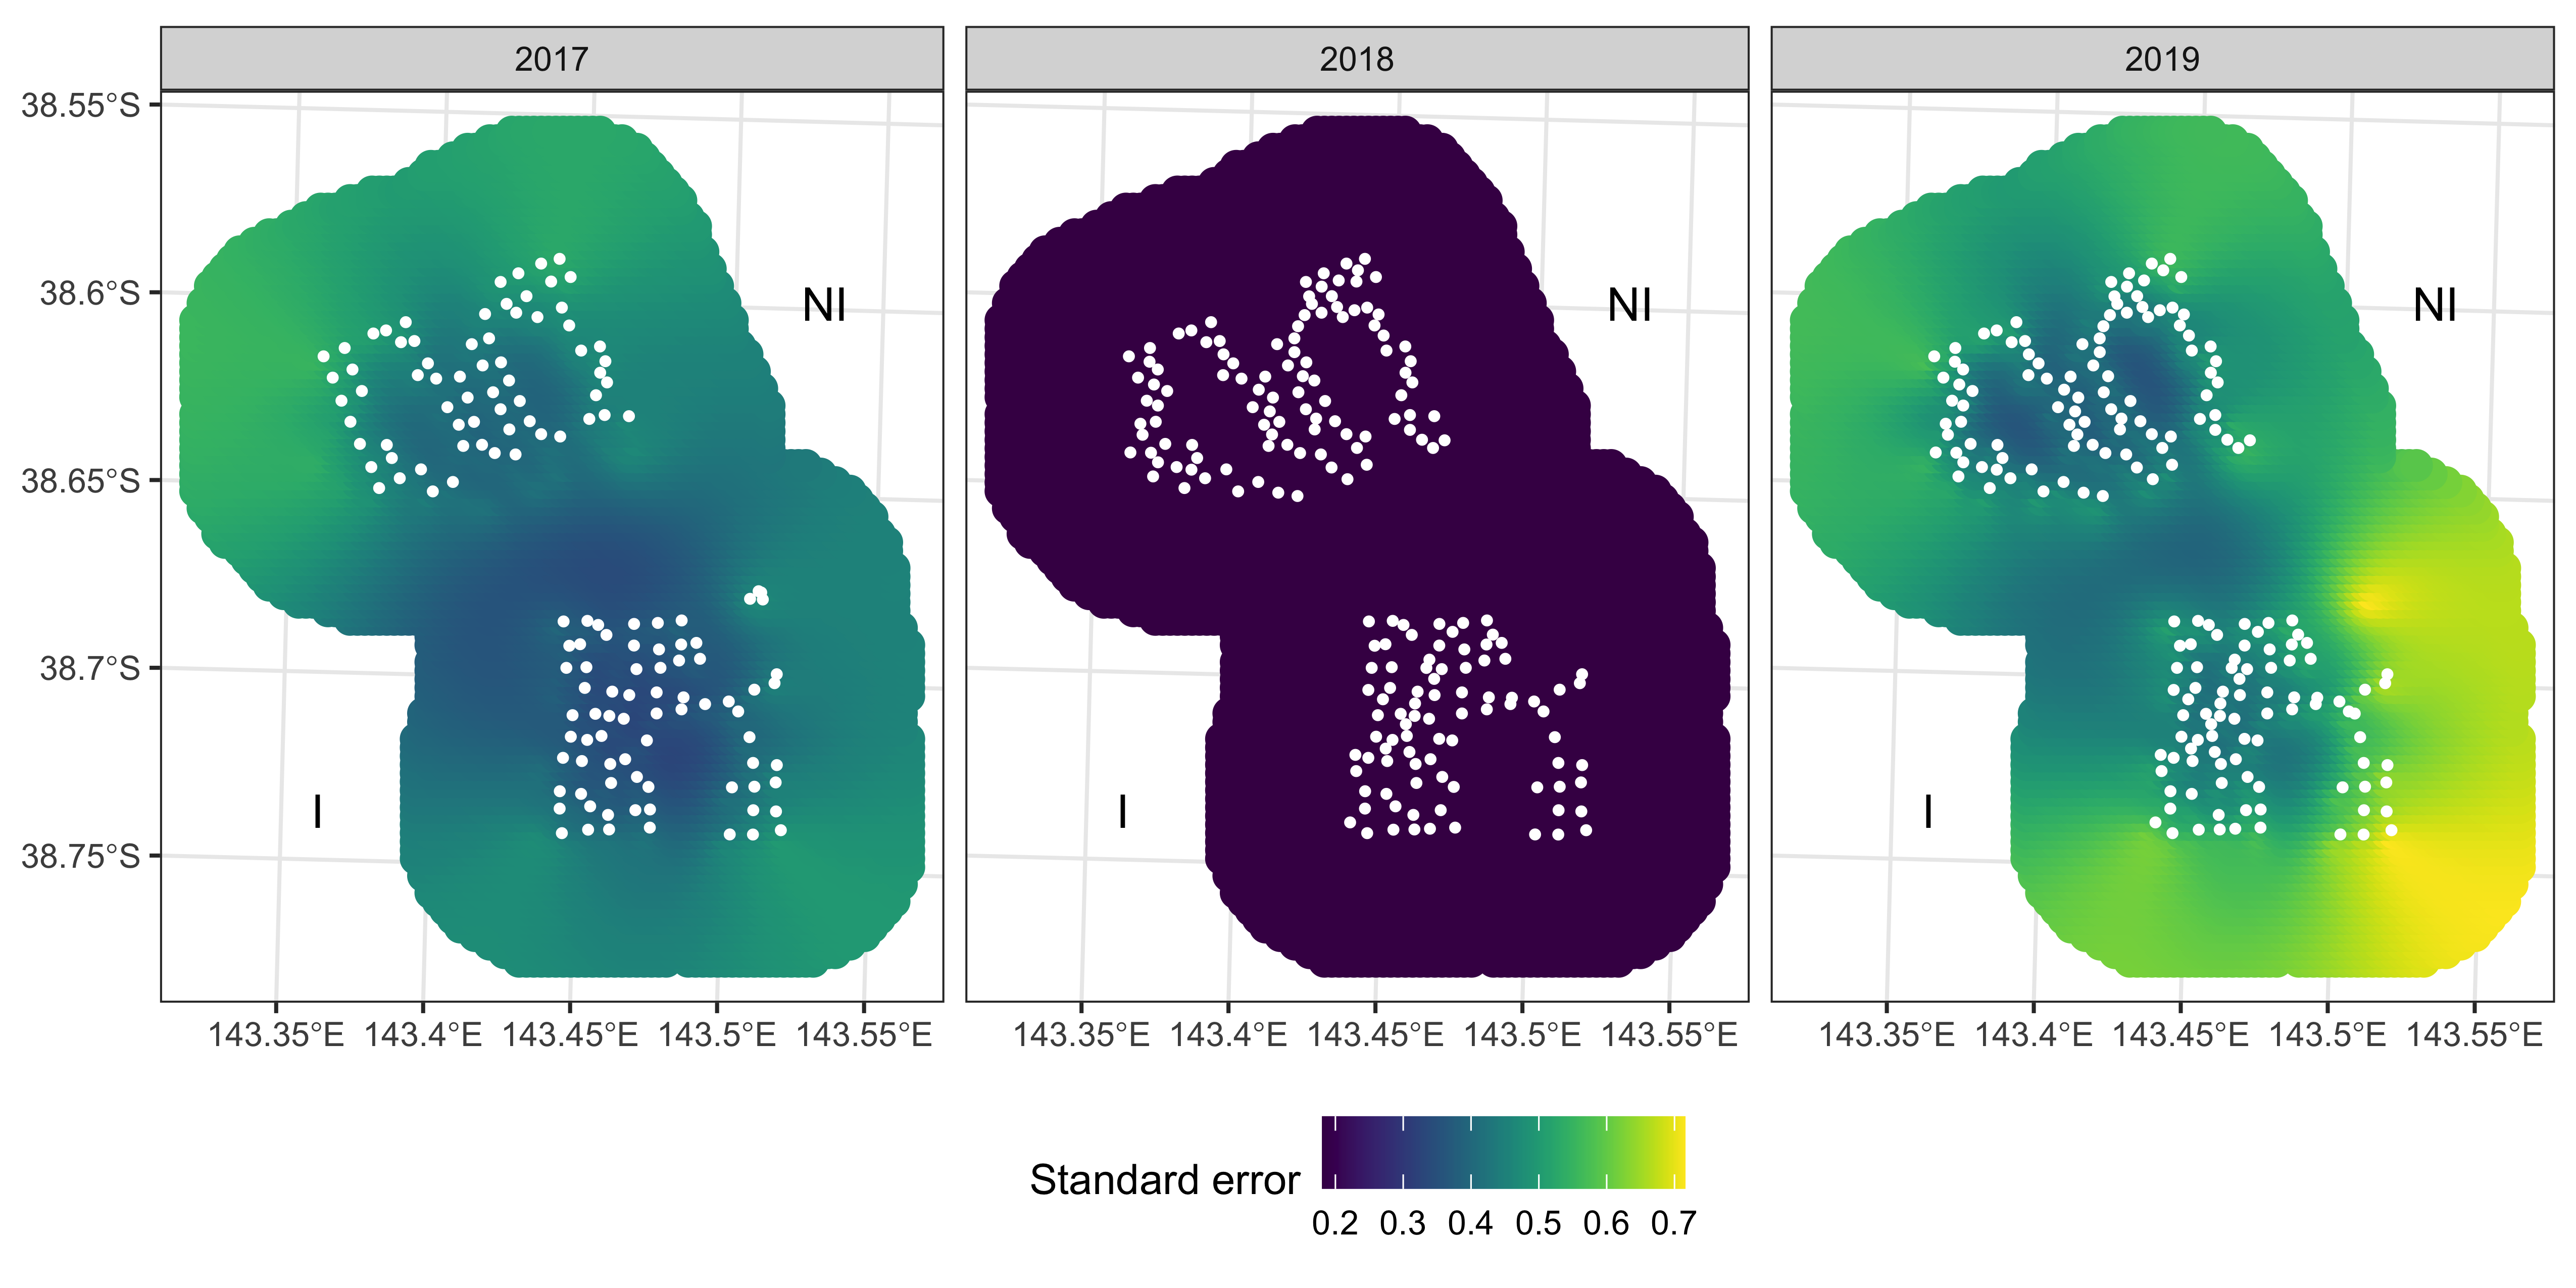
\includegraphics[width=1\linewidth]{figure/c3/fox_occ_se_otways_600dpi} 

}

\caption{Standard error estimate of log fox occurrence probability derived from generalised additive models within each impact (I) and associated non-impact (NI) landscape in the Otway region, Australia.}\label{fig:density-fox-se-o}
\end{figure}
\newpage

\hypertarget{density-app-veg}{%
\section{Vegetation categories}\label{density-app-veg}}

We condensed the main Ecological Vegetation Class groupings (DELWP 2020) present into three categories for each region: cleared land, heathy woodlands, lowland forests (Glenelg region only) and wet forests (Otways region only). We merged similar groups to reduce the number of categories for each region. In the Glenelg region, we merged dry forests with lowland forests. In the Otway region, we merged rainforests with wet forests, as well as merged dry forests and heathy woodlands.

A very small proportion of other Ecological Vegetation Class groupings were present in the habitat masks: riparian scrubs or swampy scrubs and woodlands, coastal scrubs grasslands and woodlands, wetlands, riverine grassy woodlands or forests, plains woodlands or forests, herb-rich woodlands. We removed these groups, and interpolated cell values from the nearest of the three vegetation categories.

\newpage

\(~\)

\(~\)

\(~\)
\begin{figure}

{\centering 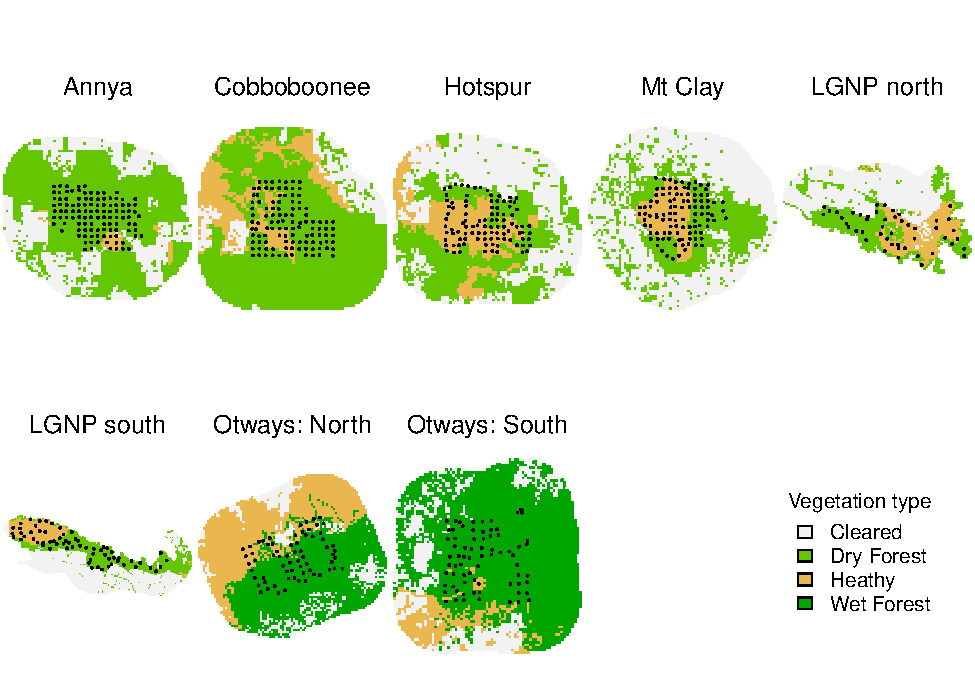
\includegraphics[width=1\linewidth]{figure/density-veg-1} 

}

\caption{Condensed Ecological Vegetation Class groups used as habitat mask covariates in spatial mark-resight models.}\label{fig:density-veg}
\end{figure}
\newpage

\hypertarget{spatial-mark-resight-models}{%
\section{Spatial mark-resight models}\label{spatial-mark-resight-models}}

\hypertarget{glenelg-region-2}{%
\subsection{Glenelg region}\label{glenelg-region-2}}

\(~\)

\(~\)

\(~\)

\begingroup\fontsize{10}{12}\selectfont
\begin{longtable}[t]{lrrrrrr}
\caption{\label{tab:density-aic-g-1}Akaike's Information Criterion values adjusted for small sample size for feral cat density models in the Glenelg region; model set 1.}\\
\toprule
Detector function & K & logLik & AIC & AICc & dAICc & AICcwt\\
\midrule
exponential & 3 & -1745.99 & 3497.99 & 3498.37 & 0.00 & 1\\
half-normal & 3 & -1763.02 & 3532.05 & 3532.43 & 34.06 & 0\\
\bottomrule
\multicolumn{7}{l}{\rule{0pt}{1em}K - number of parameters}\\
\multicolumn{7}{l}{\rule{0pt}{1em}AICc - Akaike's Information Criterion with small-sample adjustment}\\
\multicolumn{7}{l}{\rule{0pt}{1em}dAICc - difference between AICc of this model and the model with smallest AICc}\\
\multicolumn{7}{l}{\rule{0pt}{1em}AICcwt - AICc model weight}\\
\end{longtable}
\endgroup{}

\newpage

\(~\)

\(~\)

\(~\)

\begingroup\fontsize{10}{12}\selectfont
\begin{longtable}[t]{lrrrrrr}
\caption{\label{tab:density-aic-g-2}Akaike's Information Criterion values adjusted for small sample size for feral cat density models in the Glenelg region; model set 2.}\\
\toprule
Model & K & logLik & AIC & AICc & dAICc & AICcwt\\
\midrule
D\textasciitilde{}1 g0\textasciitilde{}1 sigma\textasciitilde{}1 & 3 & -1309.93 & 2625.85 & 2626.23 & 0.00 & 0.32\\
D\textasciitilde{}vegetation g0\textasciitilde{}1 sigma\textasciitilde{}1 & 5 & -1307.68 & 2625.37 & 2626.35 & 0.12 & 0.30\\
D\textasciitilde{}vegetation g0\textasciitilde{}T sigma\textasciitilde{}1 & 6 & -1306.89 & 2625.77 & 2627.17 & 0.94 & 0.20\\
D\textasciitilde{}1 g0\textasciitilde{}T sigma\textasciitilde{}1 & 4 & -1309.32 & 2626.65 & 2627.29 & 1.06 & 0.19\\
\bottomrule
\multicolumn{7}{l}{\rule{0pt}{1em}K - number of parameters}\\
\multicolumn{7}{l}{\rule{0pt}{1em}AICc - Akaike's Information Criterion with small-sample adjustment}\\
\multicolumn{7}{l}{\rule{0pt}{1em}dAICc - difference between AICc of this model and the model with smallest AICc}\\
\multicolumn{7}{l}{\rule{0pt}{1em}AICcwt - AICc model weight}\\
\multicolumn{7}{l}{\rule{0pt}{1em}T - linear time trend (g0 only)}\\
\end{longtable}
\endgroup{}

\newpage

\(~\)

\(~\)

\(~\)

\begingroup\fontsize{10}{12}\selectfont
\begin{longtable}[t]{lrrrrrr}
\caption{\label{tab:density-aic-g-3}Akaike's Information Criterion values adjusted for small sample size for feral cat density models in the Glenelg region; model set 3.}\\
\toprule
Model & K & logLik & AIC & AICc & dAICc & AICcwt\\
\midrule
D\textasciitilde{}fox\_occ g0\textasciitilde{}1 sigma\textasciitilde{}1 & 4 & -1306.67 & 2621.33 & 2621.98 & 0.00 & 0.49\\
D\textasciitilde{}fox\_occ g0\textasciitilde{}fox\_occ sigma\textasciitilde{}fox\_occ & 6 & -1304.97 & 2621.94 & 2623.34 & 1.36 & 0.25\\
D\textasciitilde{}s(fox\_occ) g0\textasciitilde{}1 sigma\textasciitilde{}1 & 5 & -1306.61 & 2623.21 & 2624.20 & 2.22 & 0.16\\
D\textasciitilde{}1 g0\textasciitilde{}1 sigma\textasciitilde{}1 & 3 & -1309.93 & 2625.85 & 2626.23 & 4.26 & 0.06\\
D\textasciitilde{}s(fox\_occ) g0\textasciitilde{}s(fox\_occ) sigma\textasciitilde{}s(fox\_occ) & 9 & -1303.41 & 2624.81 & 2627.97 & 5.99 & 0.02\\
\addlinespace
D\textasciitilde{}1 g0\textasciitilde{}fox\_occ sigma\textasciitilde{}fox\_occ & 5 & -1309.41 & 2628.82 & 2629.80 & 7.82 & 0.01\\
D\textasciitilde{}1 g0\textasciitilde{}s(fox\_occ) sigma\textasciitilde{}s(fox\_occ) & 7 & -1307.91 & 2629.81 & 2631.71 & 9.73 & 0.00\\
\bottomrule
\multicolumn{7}{l}{\rule{0pt}{1em}K - number of parameters}\\
\multicolumn{7}{l}{\rule{0pt}{1em}AICc - Akaike's Information Criterion with small-sample adjustment}\\
\multicolumn{7}{l}{\rule{0pt}{1em}dAICc - difference between AICc of this model and the model with smallest AICc}\\
\multicolumn{7}{l}{\rule{0pt}{1em}AICcwt - AICc model weight}\\
\multicolumn{7}{l}{\rule{0pt}{1em}fox\_occ - fine-scale occurrence probability of foxes derived from generalised additive models}\\
\multicolumn{7}{l}{\rule{0pt}{1em}s(fox\_occ) - non-linear smooth of fox\_occ with three knots}\\
\end{longtable}
\endgroup{}

\newpage

\(~\)

\(~\)

\(~\)

\begingroup\fontsize{10}{12}\selectfont
\begin{longtable}[t]{lrrrrrr}
\caption{\label{tab:density-aic-g-4}Akaike's Information Criterion values adjusted for small sample size for feral cat density models in the Glenelg region; model set 4.}\\
\toprule
Model & K & logLik & AIC & AICc & dAICc & AICcwt\\
\midrule
D\textasciitilde{}session g0\textasciitilde{}fox\_occ sigma\textasciitilde{}fox\_occ & 10 & -1297.46 & 2614.93 & 2618.86 & 0.00 & 0.62\\
D\textasciitilde{}session g0\textasciitilde{}1 sigma\textasciitilde{}1 & 8 & -1300.66 & 2617.32 & 2619.80 & 0.95 & 0.38\\
\bottomrule
\multicolumn{7}{l}{\rule{0pt}{1em}K - number of parameters}\\
\multicolumn{7}{l}{\rule{0pt}{1em}AICc - Akaike's Information Criterion with small-sample adjustment}\\
\multicolumn{7}{l}{\rule{0pt}{1em}dAICc - difference between AICc of this model and the model with smallest AICc}\\
\multicolumn{7}{l}{\rule{0pt}{1em}AICcwt - AICc model weight}\\
\multicolumn{7}{l}{\rule{0pt}{1em}fox\_occ - fine-scale occurrence probability of foxes derived from generalised additive models}\\
\multicolumn{7}{l}{\rule{0pt}{1em}session - landscape (n = 6)}\\
\end{longtable}
\endgroup{}

\newpage

\(~\)

\(~\)

\(~\)

\begingroup\fontsize{10}{12}\selectfont
\begin{longtable}[t]{lrrrll}
\caption{\label{tab:density-landscape-est}Feral cat density per square kilometre as estimated by the AICc top-ranked model in the Glenelg region, Australia.}\\
\toprule
Landscape & Estimate & 5\% CI & 95\% CI & Treatment & Replicate\\
\midrule
Annya & 0.24 & 0.17 & 0.34 & Non-impact & 1\\
Cobboboonee & 0.60 & 0.40 & 0.88 & Impact & 1\\
Hotspur & 0.22 & 0.14 & 0.33 & Non-impact & 2\\
Mt Clay & 0.24 & 0.18 & 0.31 & Impact & 2\\
LGNP north & 0.15 & 0.07 & 0.35 & Non-impact & 3\\
\addlinespace
LGNP south & 0.56 & 0.34 & 0.90 & Impact & 3\\
\bottomrule
\end{longtable}
\endgroup{}

\newpage

\hypertarget{otway-region-2}{%
\subsection{Otway region}\label{otway-region-2}}

\(~\)

\(~\)

\(~\)

\begingroup\fontsize{10}{12}\selectfont
\begin{longtable}[t]{lrrrrrr}
\caption{\label{tab:density-aic-o-1}Akaike's Information Criterion values for detector functions in the Otway region, Australia; model set 1.}\\
\toprule
Detector function & K & logLik & AIC & AICc & dAICc & AICcwt\\
\midrule
exponential & 3 & -5591.00 & 11188.01 & 11188.17 & 0.00 & 1\\
half-normal & 3 & -5743.26 & 11492.52 & 11492.69 & 304.52 & 0\\
\bottomrule
\multicolumn{7}{l}{\rule{0pt}{1em}K - number of parameters}\\
\multicolumn{7}{l}{\rule{0pt}{1em}AICc - Akaike's Information Criterion with small-sample adjustment}\\
\multicolumn{7}{l}{\rule{0pt}{1em}dAICc - difference between AICc of this model and the model with smallest AICc}\\
\multicolumn{7}{l}{\rule{0pt}{1em}AICcwt - AICc model weight}\\
\end{longtable}
\endgroup{}

\newpage

\(~\)

\(~\)

\(~\)

\begingroup\fontsize{10}{12}\selectfont
\begin{longtable}[t]{lrrrrrr}
\caption{\label{tab:density-aic-o-2}Akaike's Information Criterion values adjusted for small sample size for feral cat density models in the Otway region; model set 2.}\\
\toprule
Model & K & logLik & AIC & AICc & dAICc & AICcwt\\
\midrule
D\textasciitilde{}year g0\textasciitilde{}1 sigma\textasciitilde{}1 & 5 & -3550.63 & 7111.26 & 7111.67 & 0.00 & 0.48\\
D\textasciitilde{}year g0\textasciitilde{}T sigma\textasciitilde{}1 & 6 & -3549.83 & 7111.67 & 7112.25 & 0.57 & 0.36\\
D\textasciitilde{}year + vegetation g0\textasciitilde{}1 sigma\textasciitilde{}1 & 7 & -3550.04 & 7114.08 & 7114.86 & 3.19 & 0.10\\
D\textasciitilde{}year + vegetation g0\textasciitilde{}T sigma\textasciitilde{}1 & 8 & -3549.24 & 7114.48 & 7115.49 & 3.82 & 0.07\\
\bottomrule
\multicolumn{7}{l}{\rule{0pt}{1em}K - number of parameters}\\
\multicolumn{7}{l}{\rule{0pt}{1em}AICc - Akaike's Information Criterion with small-sample adjustment}\\
\multicolumn{7}{l}{\rule{0pt}{1em}dAICc - difference between AICc of this model and the model with smallest AICc}\\
\multicolumn{7}{l}{\rule{0pt}{1em}AICcwt - AICc model weight}\\
\multicolumn{7}{l}{\rule{0pt}{1em}T - linear time trend (g0 only)}\\
\end{longtable}
\endgroup{}

\newpage

\(~\)

\(~\)

\(~\)

\begingroup\fontsize{10}{12}\selectfont
\begin{longtable}[t]{lrrrrrr}
\caption{\label{tab:density-aic-o-3}Akaike's Information Criterion values adjusted for small sample size for feral cat density models in the Otway region; model set 3.}\\
\toprule
Model & K & logLik & AIC & AICc & dAICc & AICcwt\\
\midrule
D\textasciitilde{}year + fox\_occ g0\textasciitilde{}fox\_occ sigma\textasciitilde{}fox\_occ & 8 & -3541.80 & 7099.59 & 7100.60 & 0.00 & 0.33\\
D\textasciitilde{}year + s(fox\_occ) g0\textasciitilde{}s(fox\_occ) sigma\textasciitilde{}s(fox\_occ) & 11 & -3538.59 & 7099.19 & 7101.07 & 0.47 & 0.26\\
D\textasciitilde{}year g0\textasciitilde{}s(fox\_occ) sigma\textasciitilde{}s(fox\_occ) & 9 & -3541.07 & 7100.13 & 7101.40 & 0.80 & 0.22\\
D\textasciitilde{}year g0\textasciitilde{}fox\_occ sigma\textasciitilde{}fox\_occ & 7 & -3543.44 & 7100.87 & 7101.65 & 1.05 & 0.19\\
D\textasciitilde{}year + fox\_occ g0\textasciitilde{}1 sigma\textasciitilde{}1 & 6 & -3548.26 & 7108.51 & 7109.09 & 8.49 & 0.00\\
\addlinespace
D\textasciitilde{}year + s(fox\_occ) g0\textasciitilde{}1 sigma\textasciitilde{}1 & 7 & -3547.47 & 7108.94 & 7109.72 & 9.12 & 0.00\\
D\textasciitilde{}year g0\textasciitilde{}1 sigma\textasciitilde{}1 & 5 & -3550.63 & 7111.26 & 7111.67 & 11.07 & 0.00\\
\bottomrule
\multicolumn{7}{l}{\rule{0pt}{1em}K - number of parameters}\\
\multicolumn{7}{l}{\rule{0pt}{1em}AICc - Akaike's Information Criterion with small-sample adjustment}\\
\multicolumn{7}{l}{\rule{0pt}{1em}dAICc - difference between AICc of this model and the model with smallest AICc}\\
\multicolumn{7}{l}{\rule{0pt}{1em}AICcwt - AICc model weight}\\
\multicolumn{7}{l}{\rule{0pt}{1em}fox\_occ - fine-scale occurrence probability of foxes derived from generalised additive models}\\
\multicolumn{7}{l}{\rule{0pt}{1em}s(fox\_occ) - non-linear smooth of fox\_occ with three knots}\\
\end{longtable}
\endgroup{}

\newpage

\(~\)

\(~\)

\(~\)

\begingroup\fontsize{10}{12}\selectfont
\begin{longtable}[t]{lrrrrrr}
\caption{\label{tab:density-aic-o-4}Akaike's Information Criterion values adjusted for small sample size for feral cat density models in the Otway region; model set 4.}\\
\toprule
Model & K & logLik & AIC & AICc & dAICc & AICcwt\\
\midrule
D\textasciitilde{}session g0\textasciitilde{}fox\_occ sigma\textasciitilde{}fox\_occ & 10 & -3541.77 & 7103.55 & 7105.11 & 0.00 & 0.99\\
D\textasciitilde{}session g0\textasciitilde{}1 sigma\textasciitilde{}1 & 8 & -3548.37 & 7112.73 & 7113.74 & 8.63 & 0.01\\
\bottomrule
\multicolumn{7}{l}{\rule{0pt}{1em}K - number of parameters}\\
\multicolumn{7}{l}{\rule{0pt}{1em}AICc - Akaike's Information Criterion with small-sample adjustment}\\
\multicolumn{7}{l}{\rule{0pt}{1em}dAICc - difference between AICc of this model and the model with smallest AICc}\\
\multicolumn{7}{l}{\rule{0pt}{1em}AICcwt - AICc model weight}\\
\multicolumn{7}{l}{\rule{0pt}{1em}fox\_occ - fine-scale occurrence probability of foxes derived from generalised additive models}\\
\multicolumn{7}{l}{\rule{0pt}{1em}session - landscape by year (n = 6)}\\
\end{longtable}
\endgroup{}

\newpage

\(~\)

\(~\)

\(~\)

\begingroup\fontsize{10}{12}\selectfont
\begin{longtable}[t]{lrrrll}
\caption{\label{tab:density-aic-o-5}Feral cat density per square kilometre as estimated by the AICc top-ranked model in the Otway region, Australia.}\\
\toprule
Landscape & Estimate & 5\% CI & 95\% CI & Treatment & Year\\
\midrule
north 2017 & 1.00 & 0.74 & 1.35 & Non-impact & 2017\\
south 2017 & 0.74 & 0.52 & 1.05 & Impact & 2017\\
north 2018 & 0.81 & 0.64 & 1.02 & Non-impact & 2018\\
south 2018 & 0.82 & 0.63 & 1.06 & Impact & 2018\\
north 2019 & 0.73 & 0.55 & 0.95 & Non-impact & 2019\\
\addlinespace
south 2019 & 0.98 & 0.76 & 1.27 & Impact & 2019\\
\bottomrule
\end{longtable}
\endgroup{}

\newpage

\end{mainmatter}
\end{document}
